\documentclass[a4paper]{article}
\usepackage[utf8]{vietnam}
\usepackage{arxiv}
\usepackage{minted}
\usepackage{float}
\usepackage{algorithm}
\usepackage[noend]{algpseudocode}
\newcommand{\sfunction}[1]{\textsf{\textsc{#1}}}
\algrenewcommand\algorithmicforall{\textbf{foreach}}
\algrenewcommand\algorithmicindent{.8em}
\usepackage[left=3.5cm,right=2.5cm,top=2cm,bottom=2cm]{geometry}
\usepackage[hidelinks]{hyperref}
\usepackage{listings}
\hypersetup{
    colorlinks=true,
    linkcolor=black,
    filecolor=magenta,      
    urlcolor=red,
    pdftitle={Overleaf Example},
    pdfpagemode=FullScreen,
    }
\usepackage{amsmath,amssymb,amsfonts}
\usepackage{graphicx}
\usepackage[nameinlink, capitalise, noabbrev]{cleveref}
\setlength{\parindent}{0pt}
%\usepackage{wallpaper}
%\usepackage[firstpage]{draftwatermark} 
\usepackage{xcolor}
\usepackage{tikz} 
\usepackage{scrextend}
%\usepackage{background}
\usetikzlibrary{calc}
\usepackage{xcolor}
\usepackage{minted}
\usepackage[vietnamese]{babel}
\usepackage{amsmath}
\usepackage{hyperref}       % hyperlinks
\usepackage{url}            % simple URL typesetting
\usepackage{booktabs}       % professional-quality tables
\usepackage{amsfonts}       % blackboard math symbols
\usepackage{nicefrac}       % compact symbols for 1/2, etc.
\usepackage{microtype}      % microtypography
\usepackage{natbib}
\usepackage{titlesec}
\usepackage{color}
\usepackage{algorithm}
\usepackage{algpseudocode}
\setlength{\columnseprule}{1pt}
\titleformat*{\section}{\Large\bfseries}
\titleformat*{\subsection}{\Large\bfseries}
\titleformat*{\subsubsection}{\large\bfseries}
\titleformat*{\paragraph}{\large\bfseries}
\titleformat*{\subparagraph}{\large\bfseries}

\begin{document}

\begin{titlepage}

%\SetWatermarkText{\includegraphics[width = 0.97\paperwidth,
%height = 0.97\paperheight]{bia.png}}
%\SetWatermarkAngle{0} 
%\SetWatermarkText{\includegraphics[scale=1]{hust.png}}
%\SetWatermarkAngle{0} 
\begin{tikzpicture}[remember picture,overlay,inner sep=0,outer sep=0]
    \definecolor{codegreen}{rgb}{71,136,101}
     \draw[teal!70!black,line width=4pt] ([xshift=-1.5cm,yshift=-2cm]current page.north east) coordinate (A)--([xshift=1.5cm,yshift=-2cm]current page.north west) coordinate(B)--([xshift=1.5cm,yshift=2cm]current page.south west) coordinate (C)--([xshift=-1.5cm,yshift=2cm]current page.south east) coordinate(D)--cycle;

     \draw ([yshift=0.5cm,xshift=-0.5cm]A)-- ([yshift=0.5cm,xshift=0.5cm]B)--
     ([yshift=-0.5cm,xshift=0.5cm]B) --([yshift=-0.5cm,xshift=-0.5cm]B)--([yshift=0.5cm,xshift=-0.5cm]C)--([yshift=0.5cm,xshift=0.5cm]C)--([yshift=-0.5cm,xshift=0.5cm]C)-- ([yshift=-0.5cm,xshift=-0.5cm]D)--([yshift=0.5cm,xshift=-0.5cm]D)--([yshift=0.5cm,xshift=0.5cm]D)--([yshift=-0.5cm,xshift=0.5cm]A)--([yshift=-0.5cm,xshift=-0.5cm]A)--([yshift=0.5cm,xshift=-0.5cm]A);


     \draw ([yshift=-0.3cm,xshift=0.3cm]A)-- ([yshift=-0.3cm,xshift=-0.3cm]B)--
     ([yshift=0.3cm,xshift=-0.3cm]B) --([yshift=0.3cm,xshift=0.3cm]B)--([yshift=-0.3cm,xshift=0.3cm]C)--([yshift=-0.3cm,xshift=-0.3cm]C)--([yshift=0.3cm,xshift=-0.3cm]C)-- ([yshift=0.3cm,xshift=0.3cm]D)--([yshift=-0.3cm,xshift=0.3cm]D)--([yshift=-0.3cm,xshift=-0.3cm]D)--([yshift=0.3cm,xshift=-0.3cm]A)--([yshift=0.3cm,xshift=0.3cm]A)--([yshift=-0.3cm,xshift=0.3cm]A);

   \end{tikzpicture}
   
\begin{center}
    \vspace{7pt}
    \large
    \textbf{BỘ GIÁO DỤC VÀ ĐÀO TẠO}\\
    \vspace{7pt}
    \textbf{TRƯỜNG ĐẠI HỌC KINH TẾ THÀNH PHỐ HỒ CHÍ MINH}\\
    \vspace{7pt}
    \textbf{TRƯỜNG CÔNG NGHỆ VÀ THIẾT KẾ}
\end{center}
\vspace{10pt}
\begin{center}
    
\includegraphics[scale=0.3]{ueh.jpg}
    
    \vspace{20pt}
    \fontsize{14pt}{13pt}\selectfont 
    \textbf{ĐỒ ÁN MÔN HỌC}\\ 
    \vspace{5pt}
    CẤU TRÚC DỮ LIỆU VÀ GIẢI THUẬT\\
    \vspace{7pt}
\end{center}
\vspace{2cm}
\large
\textbf{ĐỀ TÀI: ỨNG DỤNG THUẬT TOÁN DIJKSTRA TỐI ƯU HOÁ CHI PHÍ VẬN TẢI}\\
\vspace{3pt}
\textbf{\large{Nhóm sinh viên thực hiện:}}
\begin{tabbing}
\hspace{8cm}\=\hspace{6cm}\=\hspace{6cm} \kill
{\textbf{Họ và tên}}\>{\textbf{MSSV}}\>{\textbf{Lớp}}\\
Nguyễn Đình Toàn \> 31211027676 \> DS001\\
Nguyễn King \> 31211023531 \> DS001\\
Đinh Trọng Hữu \> 31211027643 \> DS001\\
Nguyễn Quốc Việt \> 31211027687 \> DS001\\
\end{tabbing}
\begin{center}
\textbf{Chuyên ngành}: Khoa Học Dữ Liệu\\
\textbf{Khoá}: K47
\end{center}

\vspace{2cm}
\large
\begin{center}
    \textbf{Giảng viên:} TS. Đặng Ngọc Hoàng Thành
\end{center}
\vfill
\large
\begin{center}
    \textbf{TP Hồ Chí Minh, 2022}
\end{center}
\end{titlepage}

\large
\tableofcontents
\vfill
\pagebreak
\section{Chương 1: Đồ thị và các thuật toán}
\subsection{Các khái niệm liên quan}
Thuật toán Dijkstra là một thuật toán được dùng để tìm kiếm đường đi ngắn nhất giữa các nút (\textit{node}) trong một đồ thị có trọng số, được đề xuất đầu tiên bởi Edsger W. Dijkstra [\cite{dijkstra2022note,frana2010interview}]. Với nút trong một đồ thị cho trước, thuật toán Dijkstra tìm đường đi ngắn nhất giữa nút đó với các nút còn lại.\\

Trong đó, đồ thị là một dạng biểu diễn hình ảnh của một tập các đối tượng, các cặp đối tượng được thường được kết nối bởi các link. Các đối tượng được nối liền nhau được biểu diễn bởi các điểm được gọi là các đỉnh (node), và các link mà kết nối các đỉnh với nhau được gọi là các cạnh (edges). Cụ thể, các thành phần trong một đồ thị được định nghĩa như sau:
\begin{itemize}
    \item \textbf{Đỉnh (Node)}: Mỗi nút của hình được biểu diễn như là một đỉnh. Trong ví dụ như ở  \hyperref[fig:g1]{Hình 1}, các hình tròn biểu diễn các đỉnh. Do đó, các điểm từ 1 tới 12 là các đỉnh.
    \item \textbf{Cạnh (Edge)}: Cạnh biểu diễn một đường nối hai đỉnh. Trong hình dưới, các đường nối $1$ và $2$, $2$ và $3$, … là các cạnh. Chúng ta có thể sử dụng một mảng hai chiều để biểu diễn các cạnh này.
        \begin{figure}[!ht]
        \centering
        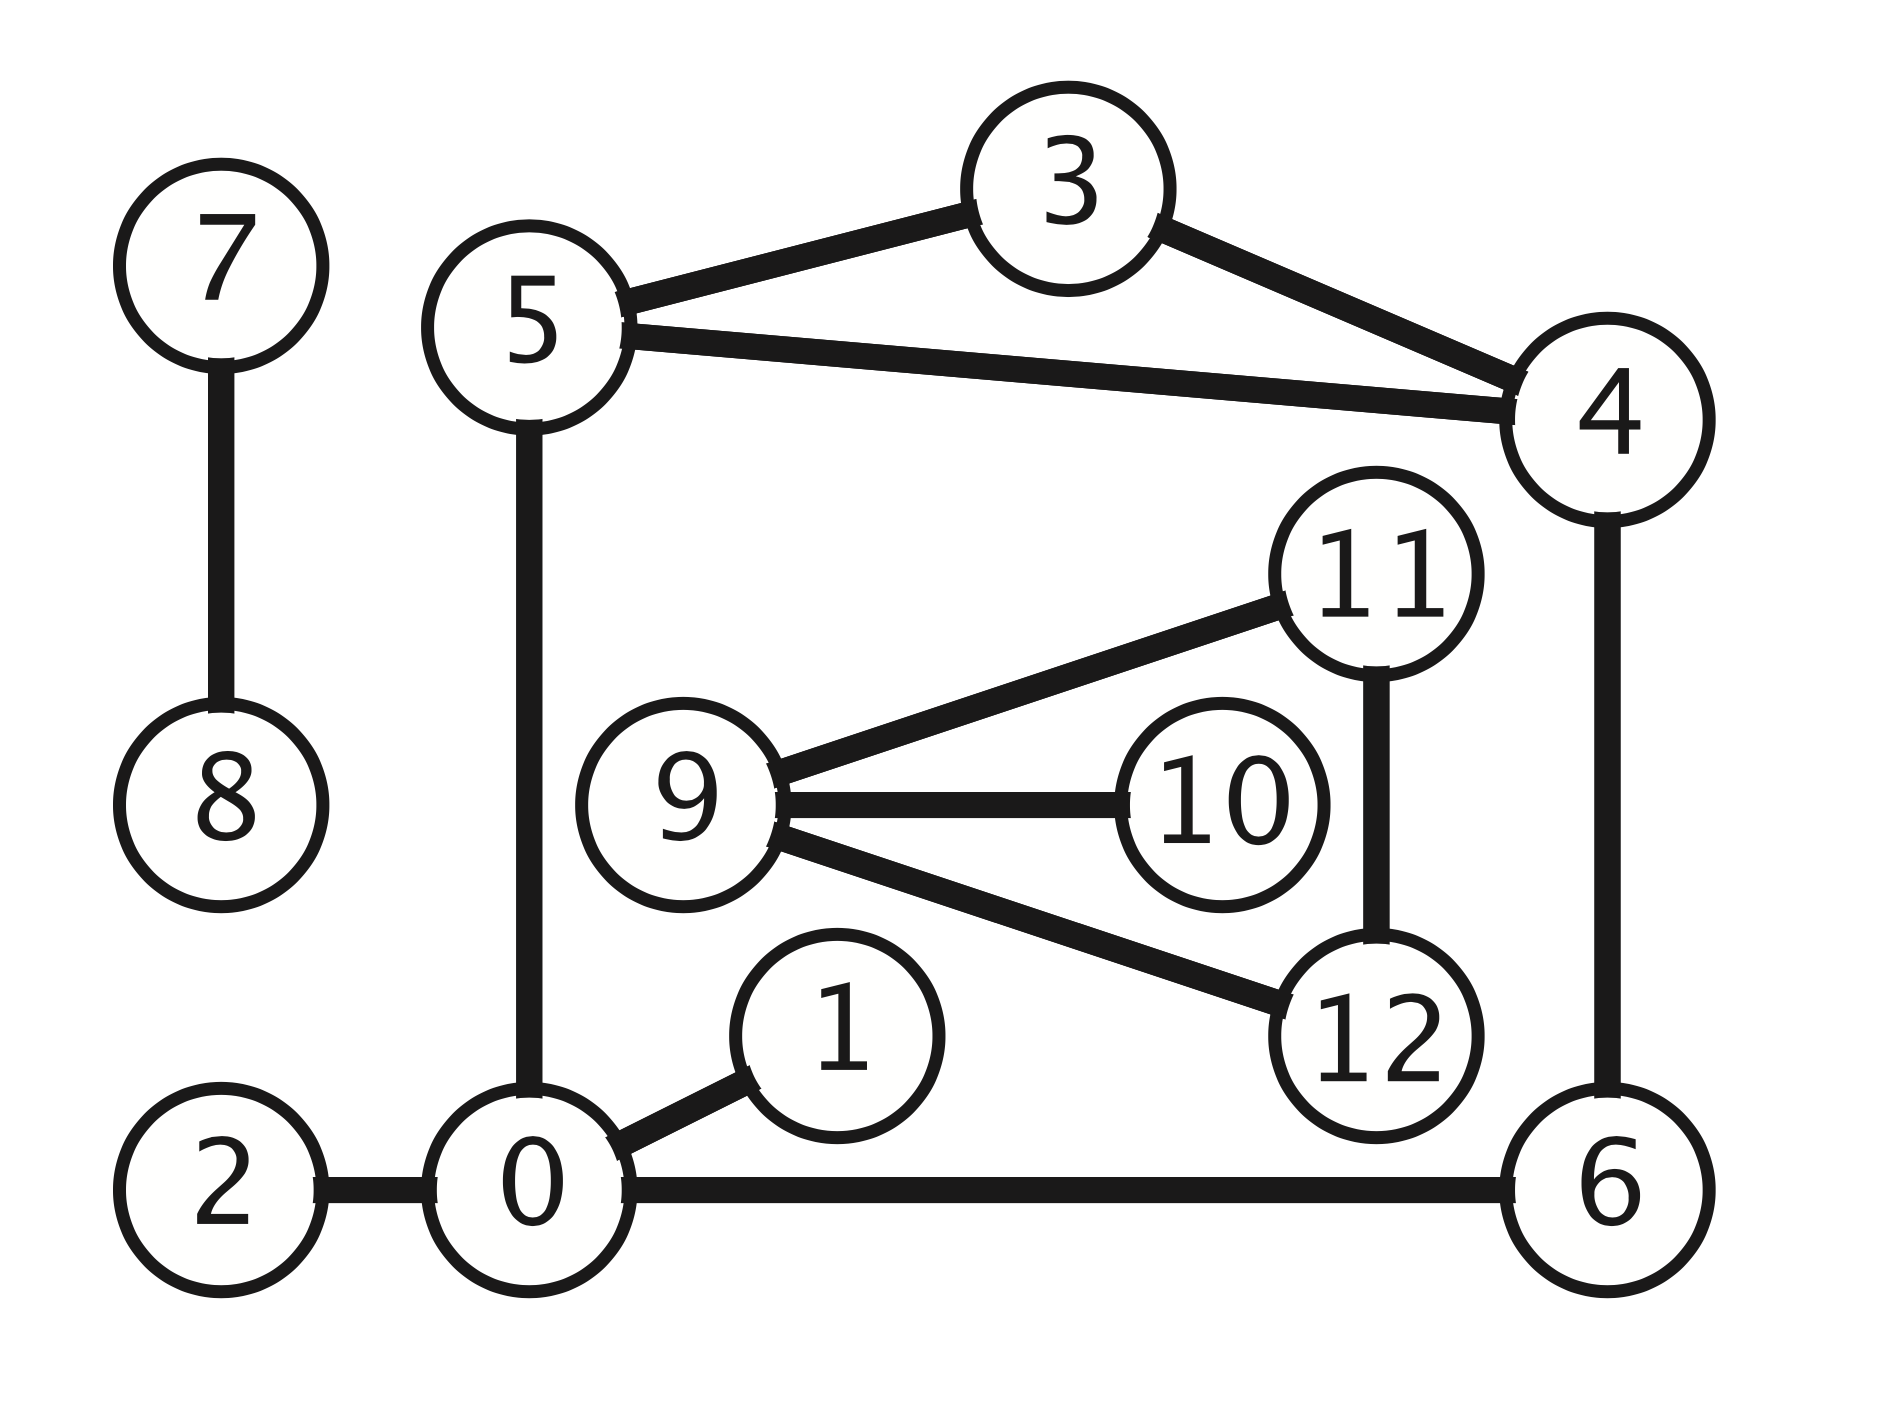
\includegraphics[width=7cm]{g1.png}
        \caption{Ví dụ về đồ thị}
        \label{fig:g1}
    \end{figure}
\end{itemize}

Đồ thị có thể được biểu diễn dưới dạng hình học hoặc dạng ma trận liền kề \textit{(adjacency matrix)}. Cụ thể, đối với một ma trận liền kề, cho $G = (V, E)$ là một đơn đồ thị có $n$ đỉnh với $V = {v_1, v_2, ..., v_{n}}$. Ma trận liền kề $\mathbf{A}$ của đồ thị $G$ là ma trận vuông cấp $n$ có các phần tử chỉ nhận một trong 2 giá trị 0 hay 1 theo nguyên tắc $a_{ik}$ là 1 nếu và chỉ nếu có cạnh kết nối đỉnh $v_{i}$ và $v_{k}$.\\

Ví dụ trong biểu diễn ma trận liền kề tương ứng với đồ thị ở \hyperref[fig:graph]{Hình 2} là :

$$ \begin{bmatrix}
0 & 1 & 1 & 1 \\
1 & 0 & 0 & 1 \\
1 & 0 & 0 & 1 \\
1 & 1 & 1 & 0 
\end{bmatrix}  $$

\begin{figure}[!ht]
    \centering
    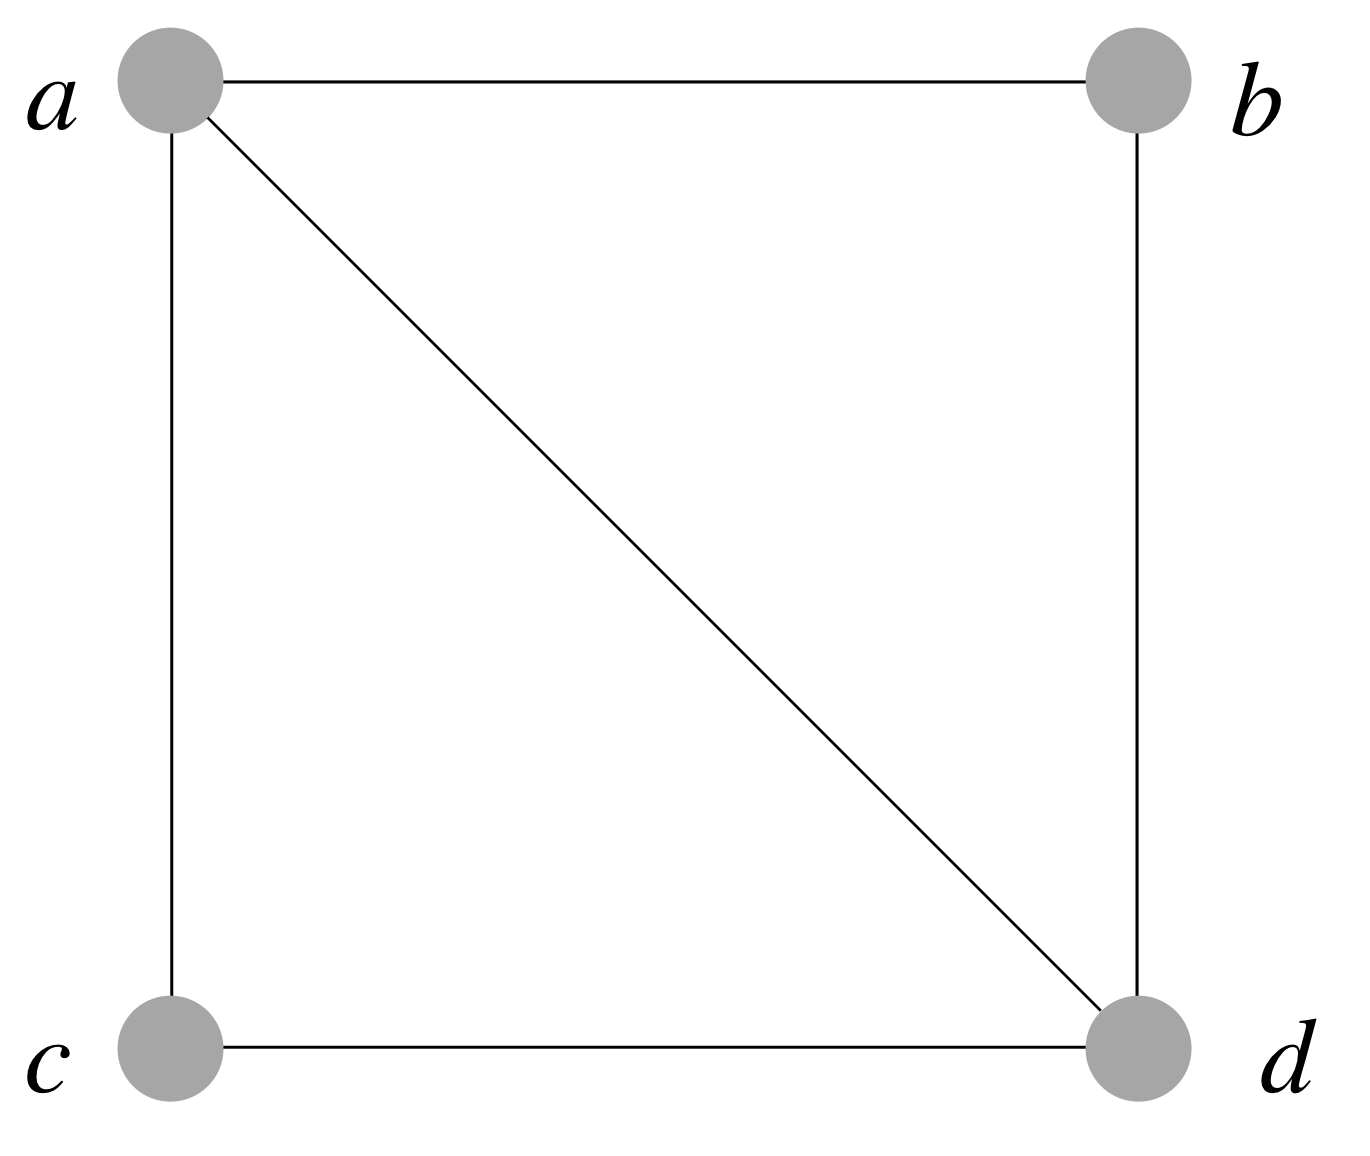
\includegraphics[width=5cm]{graph.png}
    \caption{Đồ thị tương ứng ma trận liền kề}
    \label{fig:graph}
\end{figure}

Trong thực tế, nếu các nút là biểu diễn của các thành phố và đường đi là biểu diễn của khoảng cách giữa các thành phố, thuật toán Dijkstra sẽ được sử dụng để tìm đường đi ngắn nhất giữa một thành phố đến các thành phố còn lại, hoặc để tối ưu hoá sao cho đường này là ngắn nhất [\cite{schulz2000dijkstra, chen2014path, deng2012fuzzy, makariye2017towards, bozyiugit2017public, lanning2014dijkstra}]. Về phương diện độ phức tạp tính toán, thuật toán Dijkstra là thuật toán tìm kiếm đường đi ngắn nhất trong các đồ thị có hướng với các trọng số không âm trong khoảng thời gian nhanh nhất. Trong lĩnh vực trí tuệ nhân tạo, thuật toán Dijsktra được biết đến như một thuật toán tìm kiếm chi phí cực tiểu (\textit{Uniform Cost Search}.)
\subsubsection{Cài đặt đồ thị trong C\#}
Ngôn ngữ lập trình C\# cho phép người dùng cài đặt cấu trúc đồ thị tương ứng. Cụ thể cách cài đặt các thành phần trong một cấu trúc đồ thị như sau:
\begin{itemize}
    \item Cài đặt lớp đỉnh Vertex:
    \begin{minted}[
frame=lines,
framesep=2mm,
baselinestretch=1.2,
fontsize =  \small,
linenos
]
{csharp}
public class Vertex
{
    public bool wasVisited;
    public string label;
    public Vertex(string label)
    {
        this.label = label;
        wasVisited = false;
    }
}
    \end{minted}
\item Biểu Diễn Cạnh \textit{(Edge)}
    \begin{minted}[
frame=lines,
framesep=2mm,
baselinestretch=1.2,
fontsize =  \small,
linenos
]
{csharp}
int nVertices = 0;
vertices[nVertices] = new Vertex("A");
nVertices++;
vertices[nVertices] = new Vertex("B");
nVertices++;
vertices[nVertices] = new Vertex("C");
nVertices++;
vertices[nVertices] = new Vertex("D");

adjMatrix[0,1] = 1;
adjMatrix[1,0] = 1;
adjMatrix[1,3] = 1;
adjMatrix[3,1] = 1;
    \end{minted}
\item Cài đặt lớp Đồ Thị \textit{(Graph)}
\begin{minted}[
frame=lines,
framesep=2mm,
baselinestretch=1.2,
fontsize =  \small,
linenos
]
{csharp}
public class Graph{
  int NUM_VERTICES; Vertex[] vertices;
  int[,] adjMatrix; int numVerts;
  public Graph(int number_of_vertex){
    NUM_VERTICES = number_of_vertex;
    vertices = new Vertex[NUM_VERTICES];
    adjMatrix=new int[NUM_VERTICES, NUM_VERTICES];
    numVerts = 0;
    for (int j = 0; j < NUM_VERTICES; j++)
      for (int k = 0; k < NUM_VERTICES; k++)
        adjMatrix[j, k] = 0;
  }
}
public void AddVertex(string label){
  vertices[numVerts] = new Vertex(label);
  numVerts++;
}
public void AddEdge(int start, int eend){
  adjMatrix[start, eend] = 1;
  adjMatrix[eend, start] = 1;
}
public void ShowVertex(int v){
  Console.Write(vertices[v].label + " ");
}
    \end{minted}
\end{itemize}
\subsection{Cấu trúc và cài đặt các thuật toán}
\subsubsection{Thuật toán Dijkstra}
Thuật toán Dijkstra có thể giải quyết bài toán tìm đường đi ngắn nhất trên đồ thị vô hướng lẫn có hướng miễn là trọng số không âm. Ý tưởng cơ bản của thuật toán như sau:
\begin{itemize}
\item \textbf{Ý tưởng thuật toán}
\begin{enumerate}
    \item Từ đỉnh gốc, khởi tạo khoảng cách tới chính nó là 0, khởi tạo khoảng cách nhỏ nhất ban đầu tới các đỉnh khác là $+\infty$. Ta được danh sách các khoảng cách tới các đỉnh.
    \item Chọn đỉnh $a$ có khoảng cách nhỏ nhất trong danh sách này và ghi nhận. Các lần sau sẽ không xét tới đỉnh này nữa.
    \item Lần lượt xét các đỉnh kề $b$ của đỉnh $a$. Nếu khoảng cách từ đỉnh gốc tới đỉnh $b$ nhỏ hơn khoảng cách hiện tại đang được ghi nhận thì cập nhật giá trị và đỉnh kề $a$ vào khoảng cách hiện tại của $b$.
    \item au khi xét tất cả đỉnh kề $b$ của đỉnh $a$. Lúc này ta được danh sách khoảng cách tới các điểm đã được cập nhật. Quay lại Bước 2 với danh sách này. Thuật toán kết thúc khi chọn được khoảng cách nhỏ nhất từ tất cả các điểm.
\end{enumerate}
\item \textbf{Pseudocode}
\begin{algorithm}[H]
\caption{Thuật toán Dijkstra}\label{alg:cap}
\begin{algorithmic}[1]

\Function {Dijkstra}{$Graph, source$}

    \ForAll {vertex v in Graph.Vertices:}
        \State dist[v] ← INFINITY
        \State prev[v] ← UNDEFINED
        \State add v to Q
    \EndFor
    
\State dist[source] ← 0

    \While {Q is not empty:}
        \State u ← vertex in Q with min dist[u]\
        \State remove u from Q
    \EndWhile
    
    \ForAll{neighbor v of u still in Q:}
        \State alt ← dist[u] + Graph.Edges(u, v)
        \If {alt < dist[v]:}
            \State dist[v] ← alt
            \State prev[v] ← u
        \EndIf
    \EndFor
    
\State \textbf{return} dist[], prev[]
\EndFunction
\end{algorithmic}
\end{algorithm}
\item {Cài đặt thuật toán trong C\#}
\begin{minted}[
frame=lines,
framesep=2mm,
baselinestretch=1.2,
fontsize =  \small,
linenos
]
{csharp}
public class DistOriginal
{
    public int distance;   public int parentVert;
    public DistOriginal(int pv, int d)
    {
        distance = d; parentVert = pv;
    }
}
public class Vertex
{
    public string label; public bool isInTree;
    public Vertex(string lab){label = lab; isInTree = false;}
}
public class Graph
{
    private const int max_verts = 20;
    int infinity = 1000000; Vertex[] vertexList; int[,] adjMat;
    int nVerts; int nTree; DistOriginal[] sPath;
    int currentVert; int startToCurrent;
    public Graph()
    {
        vertexList = new Vertex[max_verts];
        adjMat = new int[max_verts, max_verts];
        nVerts = 0; nTree = 0;
        for (int j = 0; j <= max_verts - 1; j++)
            for (int k = 0; k <= max_verts - 1; k++)
                adjMat[j, k] = infinity;
        sPath = new DistOriginal[max_verts];
    }
    public void AddVertex(string lab)
    {
        vertexList[nVerts] = new Vertex(lab);  nVerts++;
    }
    public void AddEdge(int start, int theEnd, int weight)
    {
        adjMat[start, theEnd] = weight;
    }
    public void Path()
    {
        int startTree = 0;
        vertexList[startTree].isInTree = true;
        nTree = 1;
        for (int j = 0; j <= nVerts; j++)
        {
            int tempDist = adjMat[startTree, j];
            sPath[j] = new DistOriginal(startTree, tempDist);
        }
        while (nTree < nVerts)
        {
            int indexMin = GetMin();
            int minDist = sPath[indexMin].distance;
            currentVert = indexMin;
            startToCurrent = sPath[indexMin].distance;
            vertexList[currentVert].isInTree = true;
            nTree++;
            AdjustShortPath();
        }
        DisplayPaths();
        nTree = 0;
        for (int j = 0; j <= nVerts - 1; j++)
            vertexList[j].isInTree = false;
    }
}
public class Graph
{
    public int GetMin()
    {
      int minDist = infinity;
      int indexMin = 0;
      for (int j = 1; j <= nVerts - 1; j++)
        if(!(vertexList[j].isInTree)&&sPath[j].distance<minDist){
            minDist = sPath[j].distance; indexMin = j;
        }
        return indexMin;
    }
    public void AdjustShortPath()
    {
        int column = 1;
        while (column < nVerts)
            if (vertexList[column].isInTree) column++;
            else
            {
              int currentToFring = adjMat[currentVert, column];
              int startToFringe = startToCurrent + currentToFring;
              int sPathDist = sPath[column].distance;
              if (startToFringe < sPathDist)
              {
                 sPath[column].parentVert = currentVert;
                 sPath[column].distance = startToFringe;
              }
              column++;
            }
    }
    public void DisplayPaths()
    {
     for (int j = 0; j <= nVerts - 1; j++)
     {
       Console.Write(vertexList[j].label + "=");
       if (sPath[j].distance == infinity) Console.Write("inf");
       else Console.Write(sPath[j].distance);
       string parent = vertexList[sPath[j].parentVert].label;
       Console.Write("(" + parent + ") ");
     }
   }
 }
\end{minted}
\end{itemize}

\subsubsection{Thuật toán Depth-first search}
\begin{itemize}
    \item \textbf{Ý tưởng thuật toán}
    \begin{enumerate}
    \item Tìm một đỉnh chưa viếng thăm nằm liên kề với đỉnh hiện tại, đánh dấu nó là đã viếng thăm và thêm vào ngăn xếp.
    \item Nếu không thể tìm thấy một đỉnh liền kề chưa được viếng thăm với đỉnh hiện tại, loại bỏ một đỉnh khỏi ngăn xếp, và bắt đầu lại.
    \item Nếu ở bước 2, ngăn xếp rỗng, thuật toán dừng.
\end{enumerate}

    \item \textbf{Cài đặt thuật toán trong C\#}
    \begin{minted}[
frame=lines,
framesep=2mm,
baselinestretch=1.2,
fontsize=\footnotesize,
linenos
]
{csharp}
private int GetAdjUnvisitedVertex(int v){
  for (int j = 0; j <= NUM_VERTICES - 1; j++)
     if((adjMatrix[v,j]==1] && (vertices[j].wasVisited==false))
         return j;
  return -1;
}
public void DepthFirstSearch(){
    vertices[0].wasVisited = true;
    ShowVertex(0);
    Stack<int> gStack = new Stack<int>();
    gStack.Push(0);
    int v; 
    while (gStack.Count > 0)
    {
        v = GetAdjUnvisitedVertex(gStack.Peek());
        if (v == -1)
            gStack.Pop();
        else
        {
            vertices[v].wasVisited = true;
            ShowVertex(v);
            gStack.Push(v);
        }
    }
    for (int j = 0; j <= NUM_VERTICES - 1; j++)
        vertices[j].wasVisited = false;
}
\end{minted}
\end{itemize}
\subsubsection{Thuật toán Breadth-first search}
\begin{itemize}
    \item \textbf{Ý tưởng thuật toán}
    \begin{enumerate}
    \item Chèn đỉnh gốc vào hàng đợi.
    \item Lấy ra đỉnh đầu tiên trong hàng đợi và quan sát nó
    \item Nếu đỉnh này chính là đỉnh đích, dừng quá trình tìm kiếm và trả về kết quả.
    \item Nếu không phải thì chèn tất cả các đỉnh kề với đỉnh vừa thăm nhưng chưa được quan sát trước đó vào hàng đợi.
    \item Nếu hàng đợi là rỗng, thì tất cả các đỉnh có thể đến được đều đã được quan sát – dừng việc tìm kiếm và trả về "không thấy".
    \item Nếu hàng đợi không rỗng thì quay về bước 2.
\end{enumerate}
    \item \textbf{Cài đặt thuật toán trong C\#}
    \begin{minted}[
frame=lines,
framesep=2mm,
baselinestretch=1.2,
fontsize=\small,
linenos
]
{csharp}
public void BreadthFirstSearch(){
    Queue<int> gQueue = new Queue<int>();
    vertices[0].wasVisited = true;
    ShowVertex(0);
    gQueue.Enqueue(0);
    int vert1, vert2;
    while (gQueue.Count > 0)
    {
        vert1 = gQueue.Dequeue();
        vert2 = GetAdjUnvisitedVertex(vert1);

     while (vert2 != -1)
     {
       vertices[vert2].wasVisited = true;
       ShowVertex(vert2);
       gQueue.Enqueue(vert2);
       vert2 = GetAdjUnvisitedVertex(vert1);
     }
    }
    for (int i=0; i <= NUM_VERTICES - 1; i++)
        vertices[index].wasVisited = false;
}
\end{minted}
\end{itemize}
\vfill
\section{Phân tích và thiết kế lớp}
\subsection{Phân tích bài toán tối ưu chi phí vận tải bằng thuật toán Dijkstra}
\textbf{Đề tài:} Giả sử chi phí vận tải giữa các địa điểm trong một quốc gia được tính toán sẵn. Xây dựng ứng dụng cho phép tìm kiếm một đường đi để chuyển hàng từ điểm A đến điểm X được chỉ định với chi phí tối thiểu.\\

Để xây dựng chương trình nhằm tối ưu hóa chi phí vận tải, ta cần một đồ thị có trọng số với các yếu tố sau:
\begin{itemize}
    \item Đỉnh: Các địa điểm trong một quốc gia (Sài Gòn, Bình Dương,…).
    \item Chi phí: Chi phí khi di chuyển trên mỗi quãng đường.
    \item Thuật toán Dijkstra tìm đường đi ngắn nhất giữa 2 địa điểm (đỉnh).
\end{itemize}
\textbf{Chi phí: }Trong bài toán tìm đường đi ngắn nhất thông thường, ta thường xem chi phí là quãng đường đi giữa 2 đỉnh. Tuy vậy, khi xây dựng ứng dụng nhằm tối ưu hóa chi phí vận tải, chi phí sẽ bao gồm các yếu tố:
\begin{itemize}
\item Số lượng xăng sử dụng
\item Tổng quãng đường di chuyển
\item Giá tiền mỗi lít xăng
Ta giả định rằng di chuyển mỗi 100km tiêu tốn 9 lít xăng và giá tiền mỗi lít xăng là 22.700 đồng. Như vậy chi phí di chuyển được tính bởi công thức:
$$\text{Chi phí} = \frac{\text{Quãng đường}}{100} \times 9 \times  22.700 \text{(đồng)}$$

\end{itemize}
\textbf{Đỉnh:} Ta tạo class Location để lưu các thông tin của mỗi địa điểm (tỉnh/thành phố).

\begin{figure}[!ht]
    \centering
    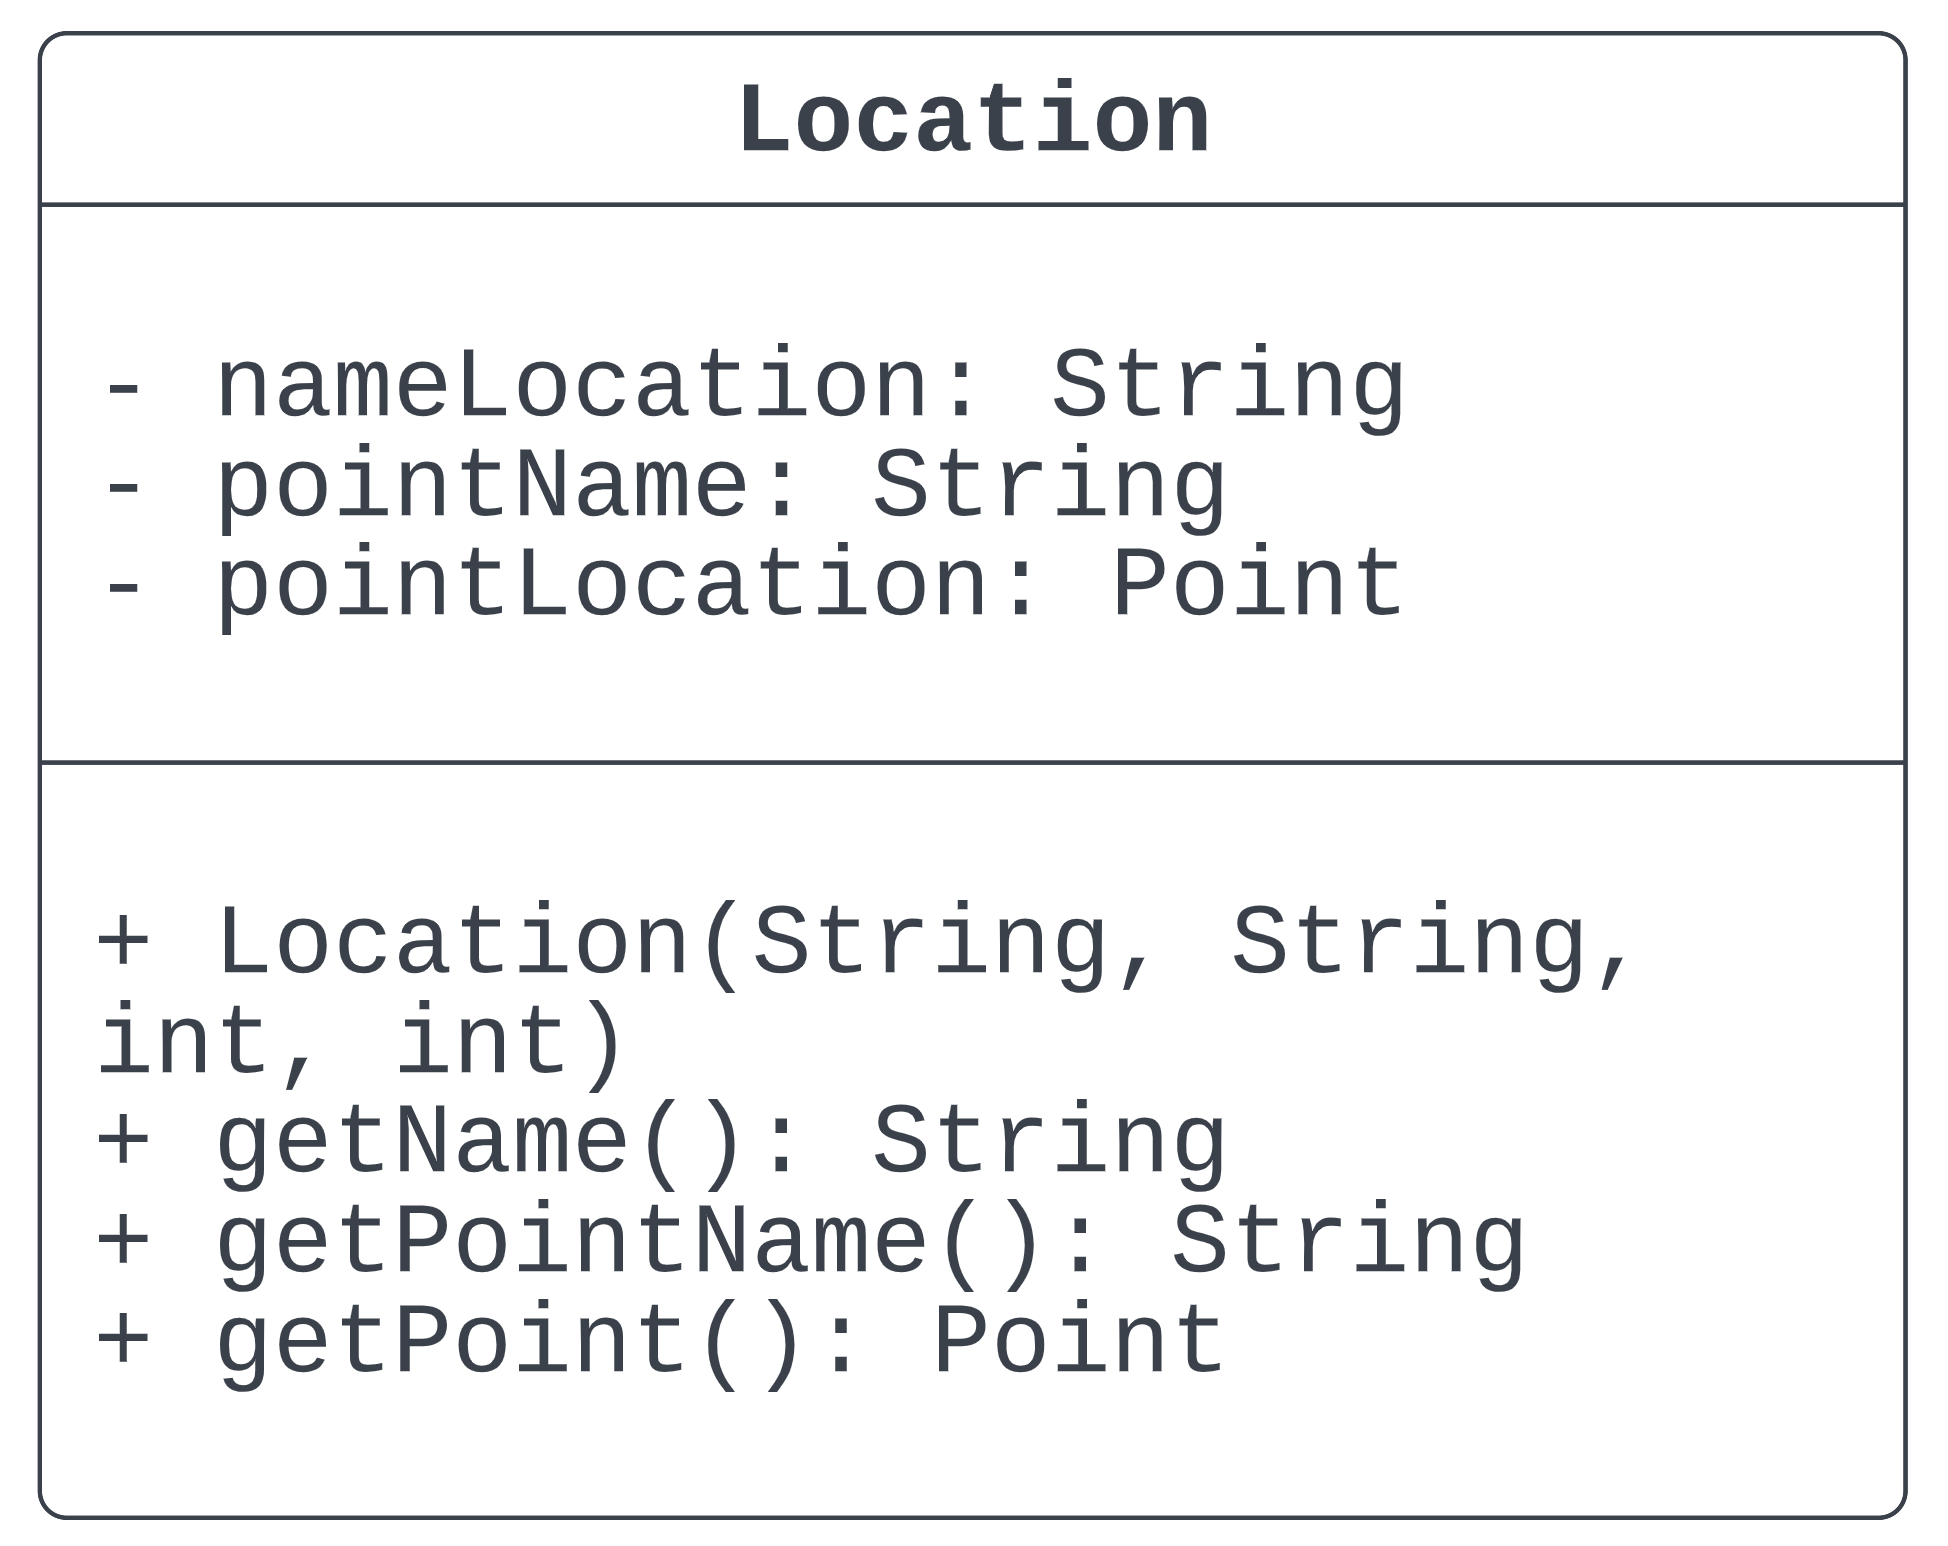
\includegraphics[width=7cm]{location.png}
    \label{fig:location}
\end{figure}

Tạo class Vertex để lưu thông tin của mỗi đỉnh trong đồ thị gồm các thuộc tính:
\begin{itemize}
\item \texttt{name:} Thể hiện tên địa điểm (tỉnh/thành phố) đại diện cho đỉnh
\item \texttt{status:} Thể hiện trạng thái của đỉnh trong quá trình thực hiện thuật toán Dijkstra (đỉnh đã được duyệt qua chưa)
\item \texttt{predecessor:} Lưu thông tin của đỉnh kề trước đỉnh hiện tại trong đường đi ngắn nhất
\item \texttt{pathLength:} Lưu thông tin đường đi ngắn nhất từ đỉnh nguồn đến đỉnh hiện tại
\end{itemize}
\begin{figure}[!ht]
    \centering
    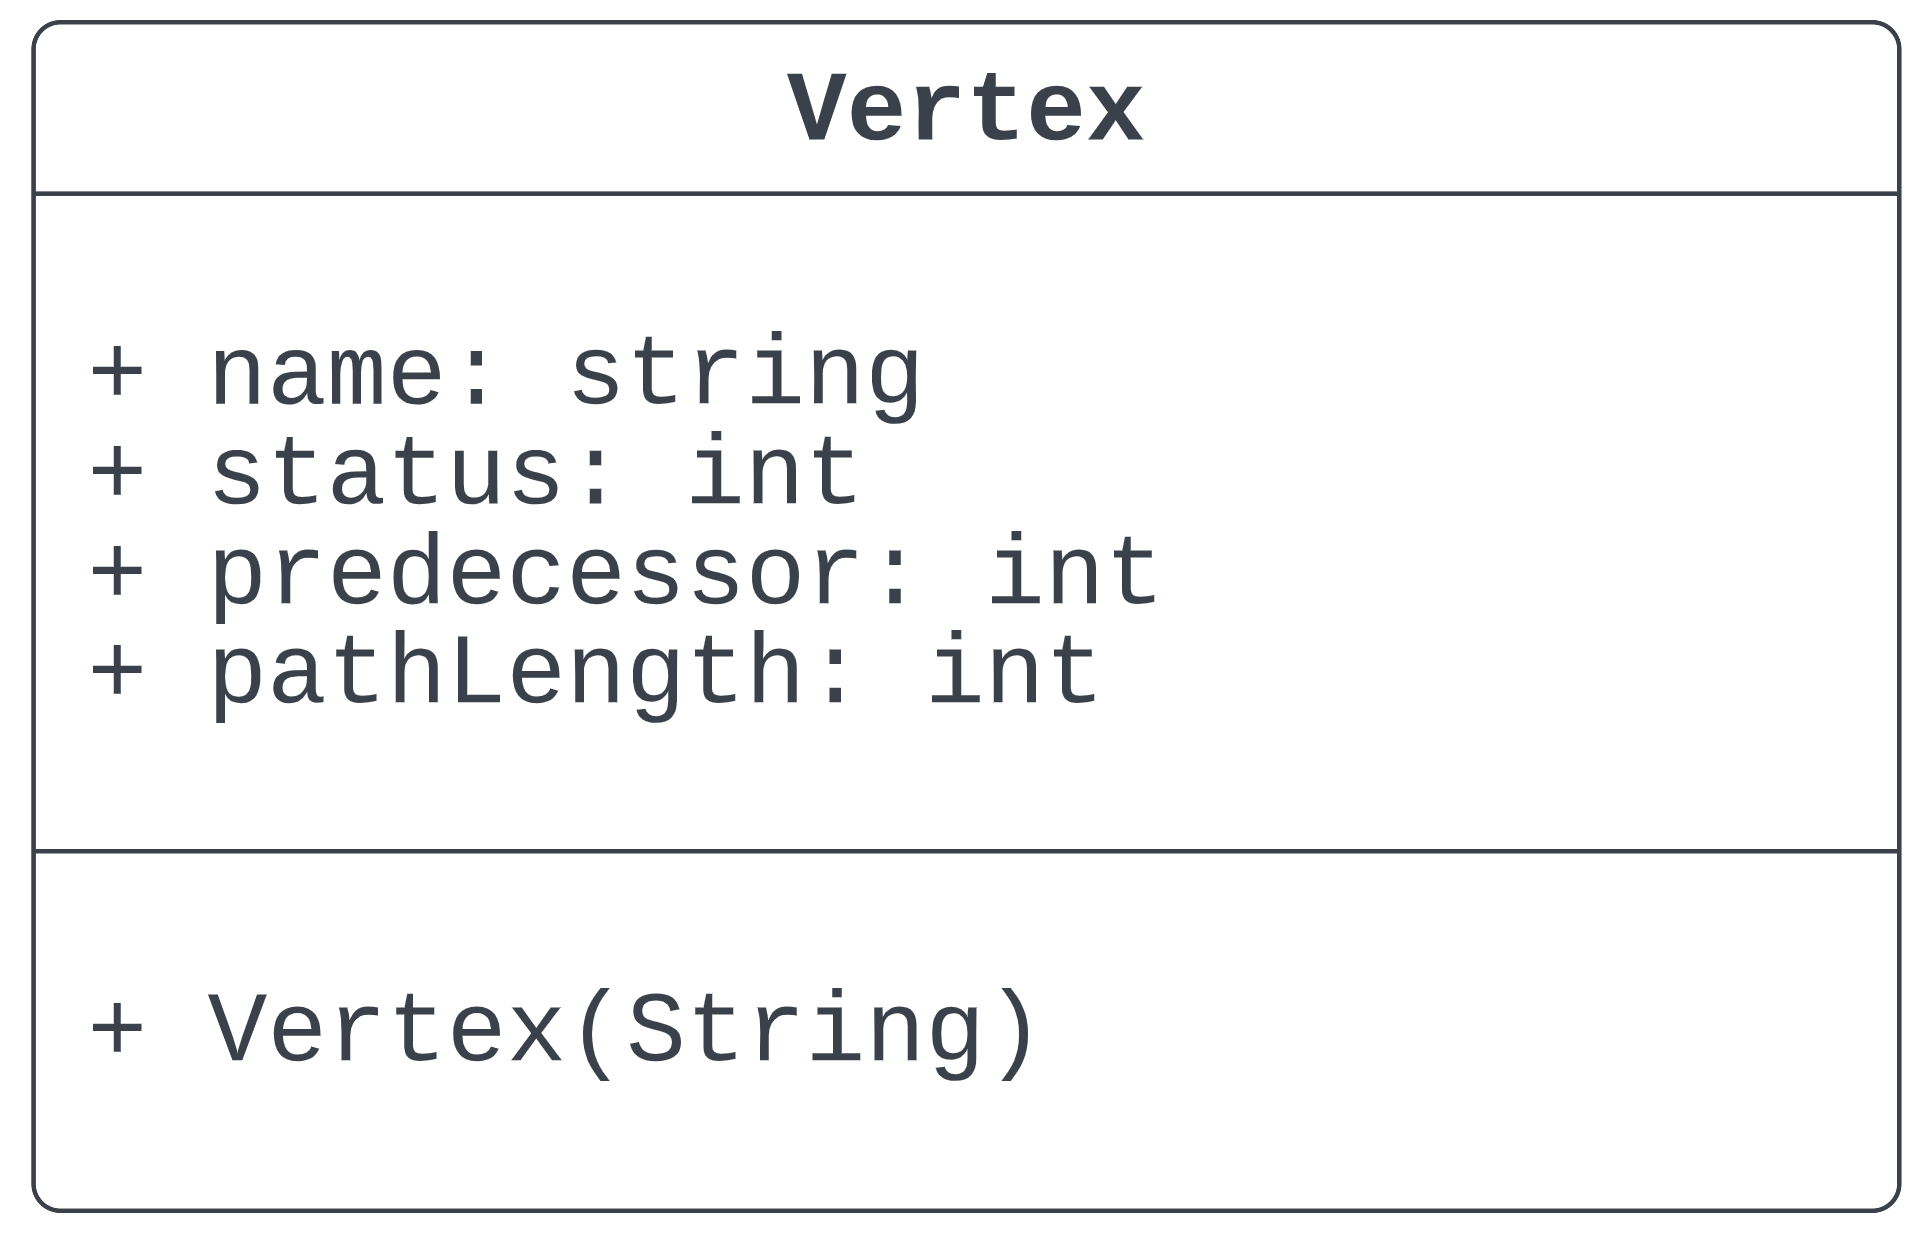
\includegraphics[width=7cm]{vertex.png}
    \label{fig:vertex}
\end{figure}

\textbf{Thuật toán Dijkstra}\\

Ta tạo class SetUpGraph để thực hiện thuật toán Dijkstra tối ưu chi phí vận tải gồm:
\begin{itemize}
    \item Thuộc tính: 
    \begin{itemize}
        \item \texttt{vertexList:} Danh sách các đỉnh
        \item \texttt{adj:} Ma trận kề lưu chi phí
        \item \texttt{listPoint:} Danh sách của các điểm trong giao diện
        \item \texttt{pathIndex:} Chỉ số của mỗi cạnh 
    \end{itemize}
    \item Phương thức: 
    \begin{itemize}
        \item \texttt{Dijkstra:} Thuật toán tìm đường đi ngắn nhất
        \item \texttt{FindPath và FindPaths:} Các phương thức thể hiện thông tin các địa điểm trong đường đi ngắn nhất
        \item \texttt{GetIndex:} Lấy chỉ số của địa điểm trong danh sách đỉnh
        \item \texttt{InsertVertex:} Thêm đỉnh
        \item \texttt{IsAdjacent:} Kiểm tra đỉnh kề
        \item \texttt{TempVertexWithMinPL:} Phương thức để tìm ra đỉnh tạm thời có đường đi ngắn nhất đến đỉnh nguồn
        \item \texttt{InsertEdge:} Phương thức thêm cạnh
    \end{itemize}
        \begin{figure}[!ht]
            \centering
            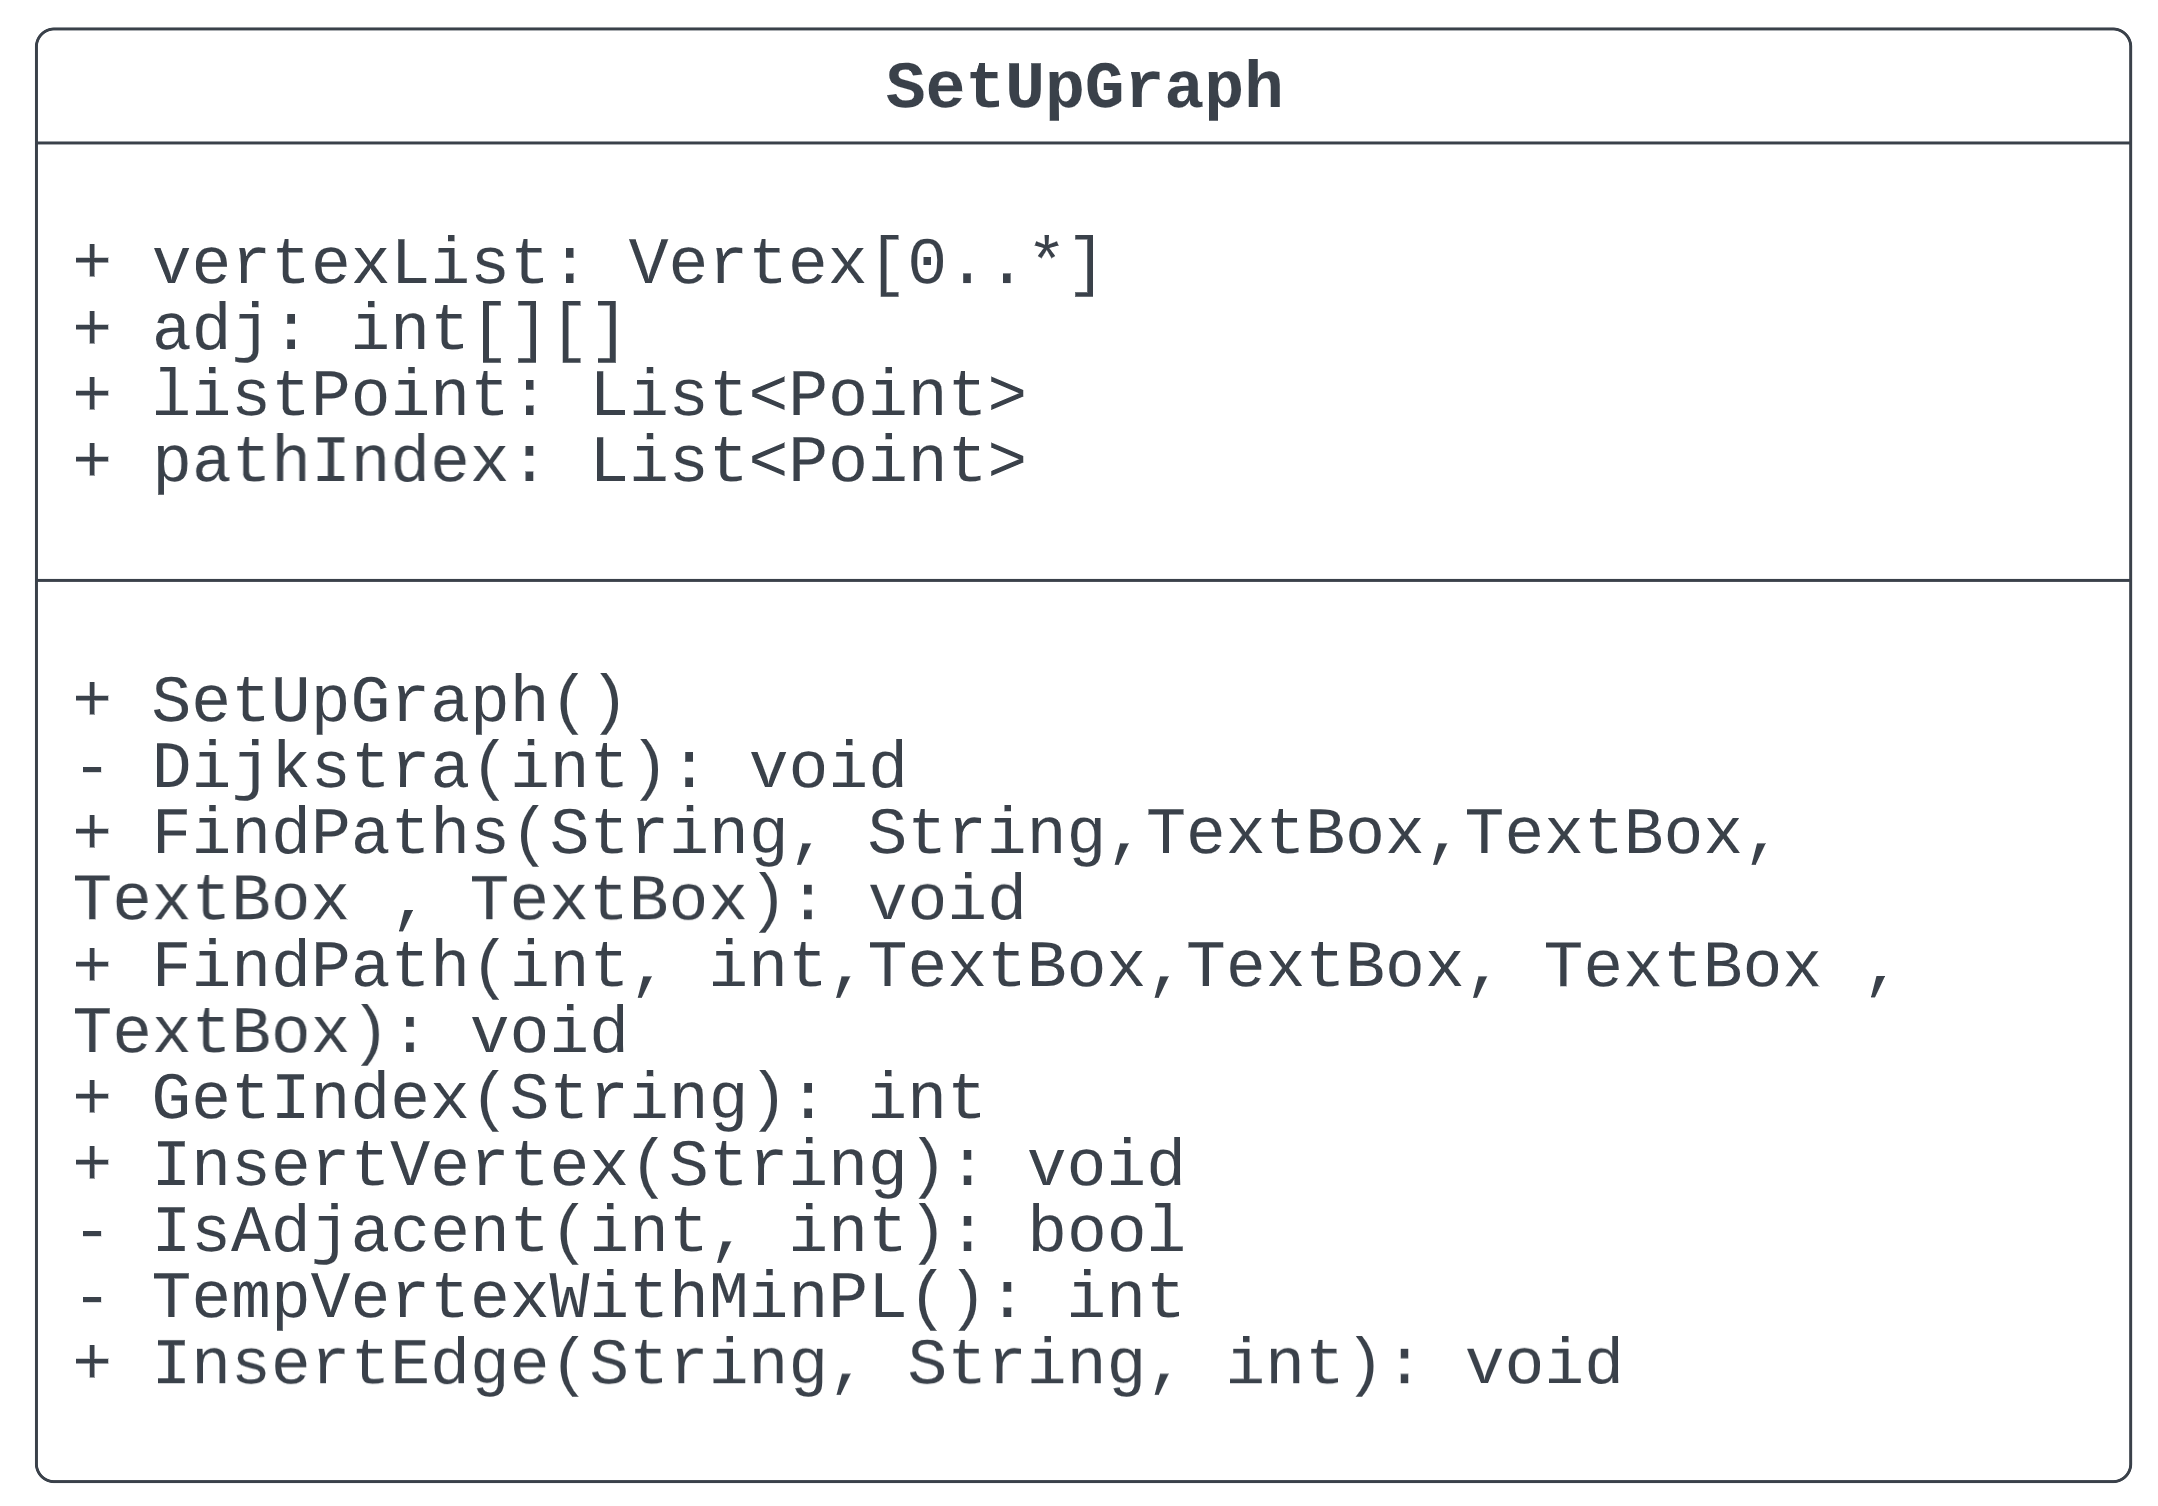
\includegraphics[width=10cm]{setup.png}
        \end{figure}
\end{itemize}
\pagebreak
\subsection{Sơ đồ lớp}

\begin{figure}[!ht]
    \centering
    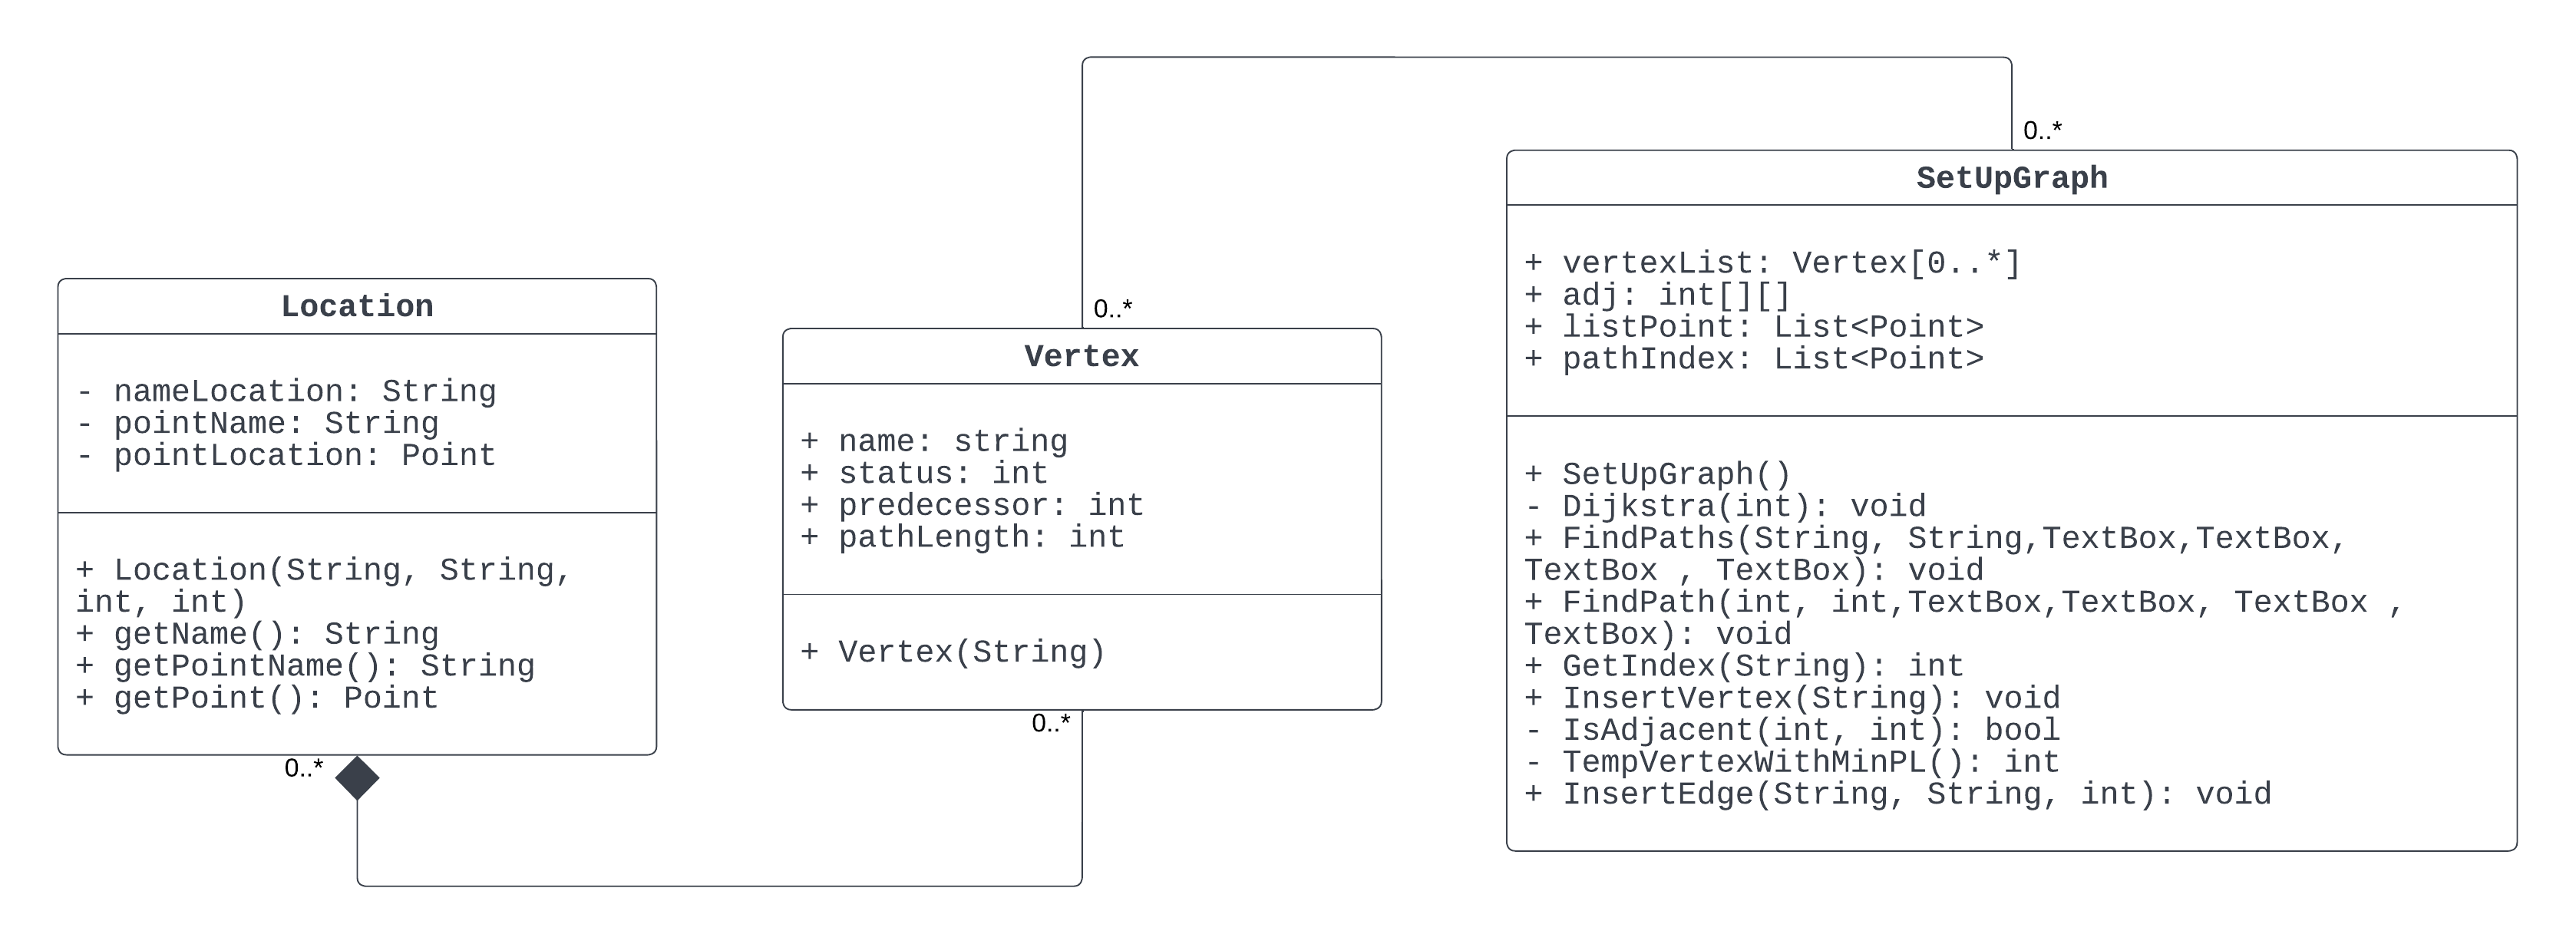
\includegraphics[width=17cm]{diagram.png}
    \caption{Sơ đồ lớp bài toán ứng dụng thuật toán Dijkstra trong tối ưu chi phí vân tải}
    \label{fig:my_label}
\end{figure}
\subsection{Cài đặt lớp}
\begin{itemize}
    \item Class Location lưu thông tin các địa điểm:
    \begin{minted}[tabsize=2,breaklines,frame=lines,framesep=2mm,baselinestretch=1.2,fontsize=\footnotesize, linenos]
{csharp}
        public class Location
    {
        private string nameLocation { get; set; }
        private string pointName { get; set; }
        private Point pointLocation { get; set; }

        public Location(string name, string symbol, int x, int y)
        {
            nameLocation = name;
            pointName = symbol;
            Point p = new Point(x, y);
            pointLocation = p;
        }
        public string getName()
        {
            return nameLocation;
        }
        public string getPointName()
        {
            return pointName;
        }
        public Point getPoint()
        {
            return pointLocation;
        }
    }
    \end{minted}
    \item Class Vertex lưu thông tin các đỉnh:
    \begin{minted}[tabsize=2,breaklines,frame=lines,framesep=2mm,baselinestretch=1.2,fontsize=\footnotesize, linenos]
{csharp}
public class Vertex
    {
        public String name;
        public int status;
        public int predecessor;
        public int pathLength;
        public Vertex(String name)
        {
            this.name = name;
        }
    }
    \end{minted}
        \item SetUpGraph:

    \begin{minted}[tabsize=2,breaklines,frame=lines,framesep=2mm,baselinestretch=1.2,fontsize=\footnotesize, linenos]
{csharp}
class SetUpGraph
    {
        public readonly int MAX_VERTICES = 100;
        public int n = 0;
        int e ;
        public int[,] adj;
        public Vertex[] vertexList;
        private readonly int INFINITY = 9999999;
        private readonly int PERMANENT = 2;
        private readonly int TEMPORARY = 1;
        private readonly int NIL = -1;
        public List<Point> listPoint = new List<Point>();
        public List<Point> pathIndex = new List<Point>();

        public SetUpGraph()
        {
            adj = new int[MAX_VERTICES, MAX_VERTICES];
            vertexList = new Vertex[MAX_VERTICES];
        }

        private void Dijkstra(int s)
        {
            int v, c;
            for (v = 0; v < n; v++)
            {
                vertexList[v].status = TEMPORARY;
                vertexList[v].pathLength = INFINITY;
                vertexList[v].predecessor = NIL;
            }
            vertexList[s].pathLength = 0;
            while (true)
            {
                c = TempVertexWithMinPL();
                if (c == NIL)
                    return;
                vertexList[c].status = PERMANENT;
                for (v = 0; v < n; v++)
                {
                    if (IsAdjacent(c, v) && vertexList[v].status == TEMPORARY)
                    {
                        if (vertexList[c].pathLength + adj[c, v] < vertexList[v].pathLength)
                        {
                            vertexList[v].predecessor = c;
                            vertexList[v].pathLength = vertexList[c].pathLength + adj[c, v];
                        }
                    }
                }
            }
        }
        public void FindPaths(string source, string last,TextBox tbKM,TextBox tbLiter, TextBox tbCost, TextBox tbPath)
        {
            int s = GetIndex(source);
            Dijkstra(s);

            int v = Convert.ToInt32(last);
            {
                if (v != s)
                {
                    if (vertexList[v].pathLength == INFINITY)
                    {
                        tbPath.Text += "\tNo path \n";
                    }
                    else
                    {
                        FindPath(s, v,tbKM, tbLiter, tbCost, tbPath);
                    }
                }
            }
        }

        public void FindPath(int s, int v, TextBox tbKM, TextBox tbLiter, TextBox tbCost, TextBox tbPath)
        {
            int i, u;
            int[] path = new int[n];
            int km = 0;
            int count = 0;
            while (v != s)
            {
                count++;
                path[count] = v;
                u = vertexList[v].predecessor;
                km += adj[u, v];
                v = u;
            }
            double sl = km * 0.09;
            int sd = km * 2043;
            count++;
            if (count >= n)
            {
                MessageBox.Show("Error!", "Notify!");

            }
            path[count] = s;
            for (i = count; i >= 1; i--)
            {
                pathIndex.Add(listPoint[path[i]]);
                if (tbPath.Text == "")
                {
                    tbPath.Text += vertexList[path[i]].name;
                }
                else
                {
                    tbPath.Text += " -> " + vertexList[path[i]].name;
                }
            }
            tbKM.Text = $"{km} KM";
            tbLiter.Text = $"{sl} liters";
            tbCost.Text = $"{sd} VNĐ";
        }

        public int GetIndex(string s)
        {
            for (int i = 0; i < n; i++)
            {
                if (s.Equals(vertexList[i].name))
                    return i;
            }
            throw new System.InvalidOperationException("Invalid Vertex");
        }

        public void InsertVertex(string name)
        {
            vertexList[n++] = new Vertex(name);
        }
        private bool IsAdjacent(int u, int v)
        {
            return adj[u, v] != 0;
        }

        private int TempVertexWithMinPL()
        {
            int min = INFINITY;
            int x = NIL;
            for (int v = 0; v < n; v++)
            {
                if (vertexList[v].status == TEMPORARY && vertexList[v].pathLength < min)
                {
                    min = vertexList[v].pathLength;
                    x = v;
                }
            }
            return x;
        }

        public void InsertEdge(string v1, string v2, int v3)
        {
            int i = GetIndex(v1);
            int j = GetIndex(v2);
            adj[i, j] = v3;
            adj[j, i] = v3;
        }
    }
    \end{minted}
\end{itemize}
\subsection{Chi tiết các phương thức}
\begin{itemize}
    \item \textbf{Phương thức Dijkstra(int s)}
\begin{itemize}
    \item Tham số đầu vào: Một số nguyên s là đỉnh (địa điểm) xuất phát.
    \item Chức năng: Thực hiện tìm đường đi ngắn nhất từ đỉnh nguồn đến mọi đỉnh trong đồ thị.
\end{itemize}

    \begin{minted}[tabsize=2,breaklines,frame=lines,framesep=2mm,baselinestretch=1.2,fontsize=\footnotesize, linenos]
{csharp}
private void Dijkstra(int s)
{
    int v, c;
    for (v = 0; v < n; v++)
    {
        vertexList[v].status = TEMPORARY;
        vertexList[v].pathLength = INFINITY;
        vertexList[v].predecessor = NIL;
    }
    vertexList[s].pathLength = 0;
    while (true)
    {
        c = TempVertexWithMinPL();
        if (c == NIL)
            return;
        vertexList[c].status = PERMANENT;
        for (v = 0; v < n; v++)
        {
            if (IsAdjacent(c, v) && vertexList[v].status == TEMPORARY)
            {
                if (vertexList[c].pathLength + adj[c, v] < vertexList[v].pathLength)
                {
                    vertexList[v].predecessor = c;
                    vertexList[v].pathLength = vertexList[c].pathLength + adj[c, v];
                }
            }
        }
    }
}
    \end{minted}

        \item \textbf{Phương thức FindPaths và FindPath} thể hiện thông tin các địa điểm trong đường đi ngắn nhất và chi phí (tổng quãng đường, số lít xăng sử dụng, tổng số tiền) trong giao diện.
    \begin{minted}[tabsize=2,breaklines,frame=lines,framesep=2mm,baselinestretch=1.2,fontsize=\footnotesize, linenos]
{csharp}
public void FindPaths(string source, string last,TextBox tbKM,TextBox tbLiter, TextBox tbCost, TextBox tbPath)
{
    int s = GetIndex(source);
    Dijkstra(s);
    int v = Convert.ToInt32(last);
    {
        if (v != s)
        {
            if (vertexList[v].pathLength == INFINITY)
            {
                tbPath.Text += "\tNo path \n";
            }
            else
            {
                FindPath(s, v,tbKM, tbLiter, tbCost, tbPath);
            }
        }
    }
}
public void FindPath(int s, int v, TextBox tbKM, TextBox tbLiter, TextBox tbCost, TextBox tbPath)
{
    int i, u;
    int[] path = new int[n];
    int km = 0;
    int count = 0;
    while (v != s)
    {
        count++;
        path[count] = v;
        u = vertexList[v].predecessor;
        km += adj[u, v];
        v = u;
    }
    double sl = km * 0.09;
    int sd = km * 2043;
    count++;
    if (count >= n)
    {
        MessageBox.Show("Error!", "Notify!");
    }
    path[count] = s;
    for (i = count; i >= 1; i--)
    {
        pathIndex.Add(listPoint[path[i]]);
        if (tbPath.Text == "")
        {
            tbPath.Text += vertexList[path[i]].name;
        }
        else
        {
            tbPath.Text += " -> " + vertexList[path[i]].name;
        }
    }
    tbKM.Text = $"{km} KM";
    tbLiter.Text = $"{sl} liters";
    tbCost.Text = $"{sd} VNĐ";
}
\end{minted}

        \item \textbf{Phương thức GetIndex(string s)}
        \begin{itemize}
            \item Tham số đầu vào: Chuỗi s thể hiện tên địa điểm (tên tỉnh/thành phố).
            \item Chức năng: Trả về một số nguyên là trị số của đỉnh đại diện cho địa điểm, nếu không tồn tại thì hiện thông báo “Invalid Vertex”.
        \end{itemize}
    \begin{minted}[tabsize=2,breaklines,frame=lines,framesep=2mm,baselinestretch=1.2,fontsize=\footnotesize, linenos]
{csharp}
public int GetIndex(string s)
        {
            for (int i = 0; i < n; i++)
            {
                if (s.Equals(vertexList[i].name))
                    return i;
            }
            throw new System.InvalidOperationException("Invalid Vertex");
        }  
    \end{minted}

        \item \textbf{Phương thức InsertVertex(string name)}
        \begin{itemize}
            \item Tham số đầu vào: Chuỗi name thể hiện tên địa điểm.
            \item Chức năng: Thực hiện nhập địa điểm thành các đỉnh trong đồ thị.
        \end{itemize}
    \begin{minted}[tabsize=2,breaklines,frame=lines,framesep=2mm,baselinestretch=1.2,fontsize=\footnotesize, linenos]
{csharp}
public void InsertVertex(string name)
        {
            vertexList[n++] = new Vertex(name);
        }
    \end{minted}

        \item \textbf{Phương thức IsAdjacent(int u, int v)}
        \begin{itemize}
            \item Tham số đầu vào: Hai số nguyên u và v là 2 đỉnh trong đồ thị.
\item Chức năng: Kiểm tra hai đỉnh u và v có phải là hai đỉnh kề không (giữa hai đỉnh có xuất hiện cạnh nối).
        \end{itemize}
    \begin{minted}[tabsize=2,breaklines,frame=lines,framesep=2mm,baselinestretch=1.2,fontsize=\footnotesize, linenos]
{csharp}
private bool IsAdjacent(int u, int v)
        {
            return adj[u, v] != 0;
        }
    \end{minted}

        \item \textbf{Phương thức TempVertexWithMinPL()}
        \begin{itemize}
            \item Tham số đầu vào: Không có
            \item Chức năng: Trả về đỉnh có quãng đường tạm thời đến đỉnh nguồn (pathLength) là ngắn nhất và chưa được viếng thăm.
        \end{itemize}
    \begin{minted}[tabsize=2,breaklines,frame=lines,framesep=2mm,baselinestretch=1.2,fontsize=\footnotesize, linenos]
{csharp}
private int TempVertexWithMinPL()
        {
            int min = INFINITY;
            int x = NIL;
            for (int v = 0; v < n; v++)
            {
                if (vertexList[v].status == TEMPORARY && vertexList[v].pathLength < min)
                {
                    min = vertexList[v].pathLength;
                    x = v;
                }
            }
            return x;
        }
    \end{minted}

        \item \textbf{Phương thức InsertEdge(string v1, string v2, int v3)}
        \begin{itemize}
            \item Tham số đầu vào: Chuỗi v1, v2 thể hiện tên của hai địa điểm có đường đi giữa chúng, số nguyên v3 thể hiện chi phí giữa hai địa điểm.
            \item Chức năng: Thực hiện lưu chi phí cạnh (đường đi) vào ma trận kề.
        \end{itemize}
    \begin{minted}[tabsize=2,breaklines,frame=lines,framesep=2mm,baselinestretch=1.2,fontsize=\footnotesize, linenos]
{csharp}
public void InsertEdge(string v1, string v2, int v3)
        {
            int i = GetIndex(v1);
            int j = GetIndex(v2);
            adj[i, j] = v3;
            adj[j, i] = v3;
        }
    \end{minted}
\end{itemize}
\section{Thiết kế giao diện} \label{p3}
\subsection{Giao diện menu chính}
\begin{minted}[tabsize=2,breaklines,frame=lines,framesep=2mm,baselinestretch=1.2,fontsize=\footnotesize, linenos]
{csharp}
namespace DijkstraTest2
{
    public partial class Form1 : Form
    {
        public Form1()
        {
            InitializeComponent();
        }

        public List<Location> Locations = new List<Location>();
        SetUpGraph g = new SetUpGraph();
        private void Form1_Load(object creator, EventArgs e) //Goi ten cac dia diem va set vi tri
        {
            Location binhPhuoc = new Location("Bình Phước", "A", 541, 65);
            Location saiGon = new Location("Sài Gòn", "B", 502, 164);
            Location tayNinh = new Location("Tây Ninh", "C", 431, 105);
            Location vungTau = new Location("Vũng Tàu", "D", 590, 198);
            Location tienGiang = new Location("Tiền Giang", "E", 432, 212);
            Location anGiang = new Location("An Giang", "F", 296, 210);
            Location hauGiang = new Location("Hậu Giang", "G", 348, 286);
            Location traVinh = new Location("Trà Vinh", "H", 462, 286);
            Location kienGiang = new Location("Kiên Giang", "I", 290, 286);
            Location caMau = new Location("Cà Mau", "K", 260, 345);
            Locations.Add(binhPhuoc);
            Locations.Add(saiGon);
            Locations.Add(tayNinh);
            Locations.Add(vungTau);
            Locations.Add(tienGiang);
            Locations.Add(anGiang);
            Locations.Add(hauGiang);
            Locations.Add(traVinh);
            Locations.Add(kienGiang);
            Locations.Add(caMau);
            cbSource.Items.Add("Bình Phước");
            cbSource.Items.Add("Sài Gòn");
            cbSource.Items.Add("Tây Ninh");
            cbSource.Items.Add("Vũng Tàu");
            cbSource.Items.Add("Tiền Giang");
            cbSource.Items.Add("An Giang");
            cbSource.Items.Add("Hậu Giang");
            cbSource.Items.Add("Trà Vinh");
            cbSource.Items.Add("Kiên Giang");
            cbSource.Items.Add("Cà Mau");
            cbDestination.Items.Add("Bình Phước");
            cbDestination.Items.Add("Sài Gòn");
            cbDestination.Items.Add("Tây Ninh");
            cbDestination.Items.Add("Vũng Tàu");
            cbDestination.Items.Add("Tiền Giang");
            cbDestination.Items.Add("An Giang");
            cbDestination.Items.Add("Hậu Giang");
            cbDestination.Items.Add("Trà Vinh");
            cbDestination.Items.Add("Kiên Giang");
            cbDestination.Items.Add("Cà Mau");
            Graphics graph = southMap.CreateGraphics();
            for (int i = 0; i < Locations.Count; i++)
            {
                lvListProvinces.Items.Add(Locations[i].getPointName());
                lvListProvinces.Items[i].SubItems.Add(Locations[i].getName());
                g.listPoint.Add(Locations[i].getPoint());
                g.InsertVertex(Locations[i].getName());
            }
            g.InsertEdge("Tây Ninh", "Bình Phước", 111);
            g.InsertEdge("Vũng Tàu", "Bình Phước", 182);
            g.InsertEdge("Sài Gòn", "Bình Phước", 124);
            g.InsertEdge("Vũng Tàu", "Sài Gòn", 98);
            g.InsertEdge("Tiền Giang", "Sài Gòn", 72);
            g.InsertEdge("An Giang", "Sài Gòn", 235);
            g.InsertEdge("Tây Ninh", "Sài Gòn", 92);
            g.InsertEdge("Trà Vinh", "Sài Gòn", 125);
            g.InsertEdge("Trà Vinh", "Cà Mau", 195);
            g.InsertEdge("Trà Vinh", "Hậu Giang", 124);
            g.InsertEdge("Tiền Giang", "An Giang", 174);
            g.InsertEdge("Trà Vinh", "Tiền Giang", 68);
            g.InsertEdge("An Giang", "Trà Vinh", 187);
            g.InsertEdge("Hậu Giang", "Cà Mau", 130);
            g.InsertEdge("Cà Mau", "Kiên Giang", 106);
            g.InsertEdge("An Giang", "Hậu Giang", 146);
            g.InsertEdge("An Giang", "Kiên Giang", 96);
        }
        //Vẽ bản đồ ra Panel
        private void southMap_Paint(object creator, PaintEventArgs e)
        {
            Graphics graph = southMap.CreateGraphics();
            for (int i = 0; i < Locations.Count; i++)
            {
                SolidBrush brush = new SolidBrush(Color.SeaGreen);
                Brush pointName = new SolidBrush(Color.White);
                graph.FillEllipse(brush, Locations[i].getPoint().X - 3, Locations[i].getPoint().Y - 2, 18, 18);
                graph.DrawString(Locations[i].getPointName(), new Font("Arial", 8), pointName, Locations[i].getPoint().X, Locations[i].getPoint().Y);
            }
            DrawLine();
        }

        private void DrawLine() // Noi cac tuyen duong co the di duoc va da tinh toan chi phi
        {
            DrawLine("Tây Ninh", "Bình Phước");
            DrawLine("Vũng Tàu", "Bình Phước");
            DrawLine("Sài Gòn", "Bình Phước");
            DrawLine("Vũng Tàu", "Sài Gòn");
            DrawLine("Tiền Giang", "Sài Gòn");
            DrawLine("An Giang", "Sài Gòn");
            DrawLine("Tây Ninh", "Sài Gòn");
            DrawLine("Trà Vinh", "Sài Gòn");
            DrawLine("Trà Vinh", "Cà Mau");
            DrawLine("Trà Vinh", "Hậu Giang");
            DrawLine("Tiền Giang", "An Giang");
            DrawLine("Trà Vinh", "Tiền Giang");
            DrawLine("An Giang", "Trà Vinh");
            DrawLine("Hậu Giang", "Cà Mau");
            DrawLine("Cà Mau", "Kiên Giang");
            DrawLine("An Giang", "Hậu Giang");
            DrawLine("An Giang", "Kiên Giang");
        }
        private void DrawLine(string a, string b)
        {
            Graphics graph = southMap.CreateGraphics();
            int x = g.GetIndex(a);
            int y = g.GetIndex(b);
            Pen p = new Pen(Color.Black, 2);
            Point point1 = new Point(g.listPoint[x].X, g.listPoint[x].Y);
            Point point2 = new Point(g.listPoint[y].X, g.listPoint[y].Y);
            graph.DrawLine(p, point1, point2);
            graph.DrawString($"{g.adj[x, y]}", new Font("Fira Code", 10), Brushes.Black, new Point((point1.X + point2.X) / 2 - 8, (point1.Y + point2.Y) / 2 + 8));
        }
        private void cbSource_SelectedIndexChanged(object creator, EventArgs e)
        {
            if (cbSource.SelectedIndex != -1 && cbDestination.SelectedIndex != -1)
            {
                southMap.Controls.Clear();
                southMap.Refresh();
                DrawLine();
                g.pathIndex.Clear();
                tbKM.Clear();
                tbLiter.Clear();
                tbCost.Clear();
                tbPath.Clear();
                g.FindPaths(cbSource.SelectedItem.ToString(), cbDestination.SelectedIndex.ToString(),tbKM,tbLiter, tbCost, tbPath);
                for (int i = 0; i < g.pathIndex.Count - 1; i++)
                {
                    DrawPathLine(i);
                }
            }
            if (cbSource.SelectedIndex == cbDestination.SelectedIndex)
            {
                MessageBox.Show("Unresponsive\n The location can't be the same !", "Notify!");
            }
        }
        private void cbDestination_SelectedIndexChanged(object creator, EventArgs e)
        {
            if (cbSource.SelectedIndex != -1 && cbDestination.SelectedIndex != -1)
            {
                southMap.Controls.Clear();
                southMap.Refresh();
                DrawLine();
                g.pathIndex.Clear();
                tbKM.Clear();
                tbLiter.Clear();
                tbCost.Clear();
                tbPath.Clear();
                g.FindPaths(cbSource.SelectedItem.ToString(), cbDestination.SelectedIndex.ToString(),tbKM ,tbLiter, tbCost, tbPath);
                for (int i = 0; i < g.pathIndex.Count - 1; i++)
                {
                    DrawPathLine(i);
                }
            }
            if (cbSource.SelectedIndex == cbDestination.SelectedIndex)
            {
                MessageBox.Show("Unresponsive\n The location can't be the same !", "Notify!");
            }    
        }
        //Vẽ lại đường đi ngắn nhất
        private void DrawPathLine(int i)
        {
            Graphics graph = southMap.CreateGraphics();
            Pen p = new Pen(Color.Aqua, 2);
            Point point1 = new Point(g.pathIndex[i].X, g.pathIndex[i].Y);
            Point point2 = new Point(g.pathIndex[i + 1].X, g.pathIndex[i + 1].Y);
            graph.DrawLine(p, point1, point2);
        }

    }
}
\end{minted}
\begin{figure}[!ht]
    \centering
    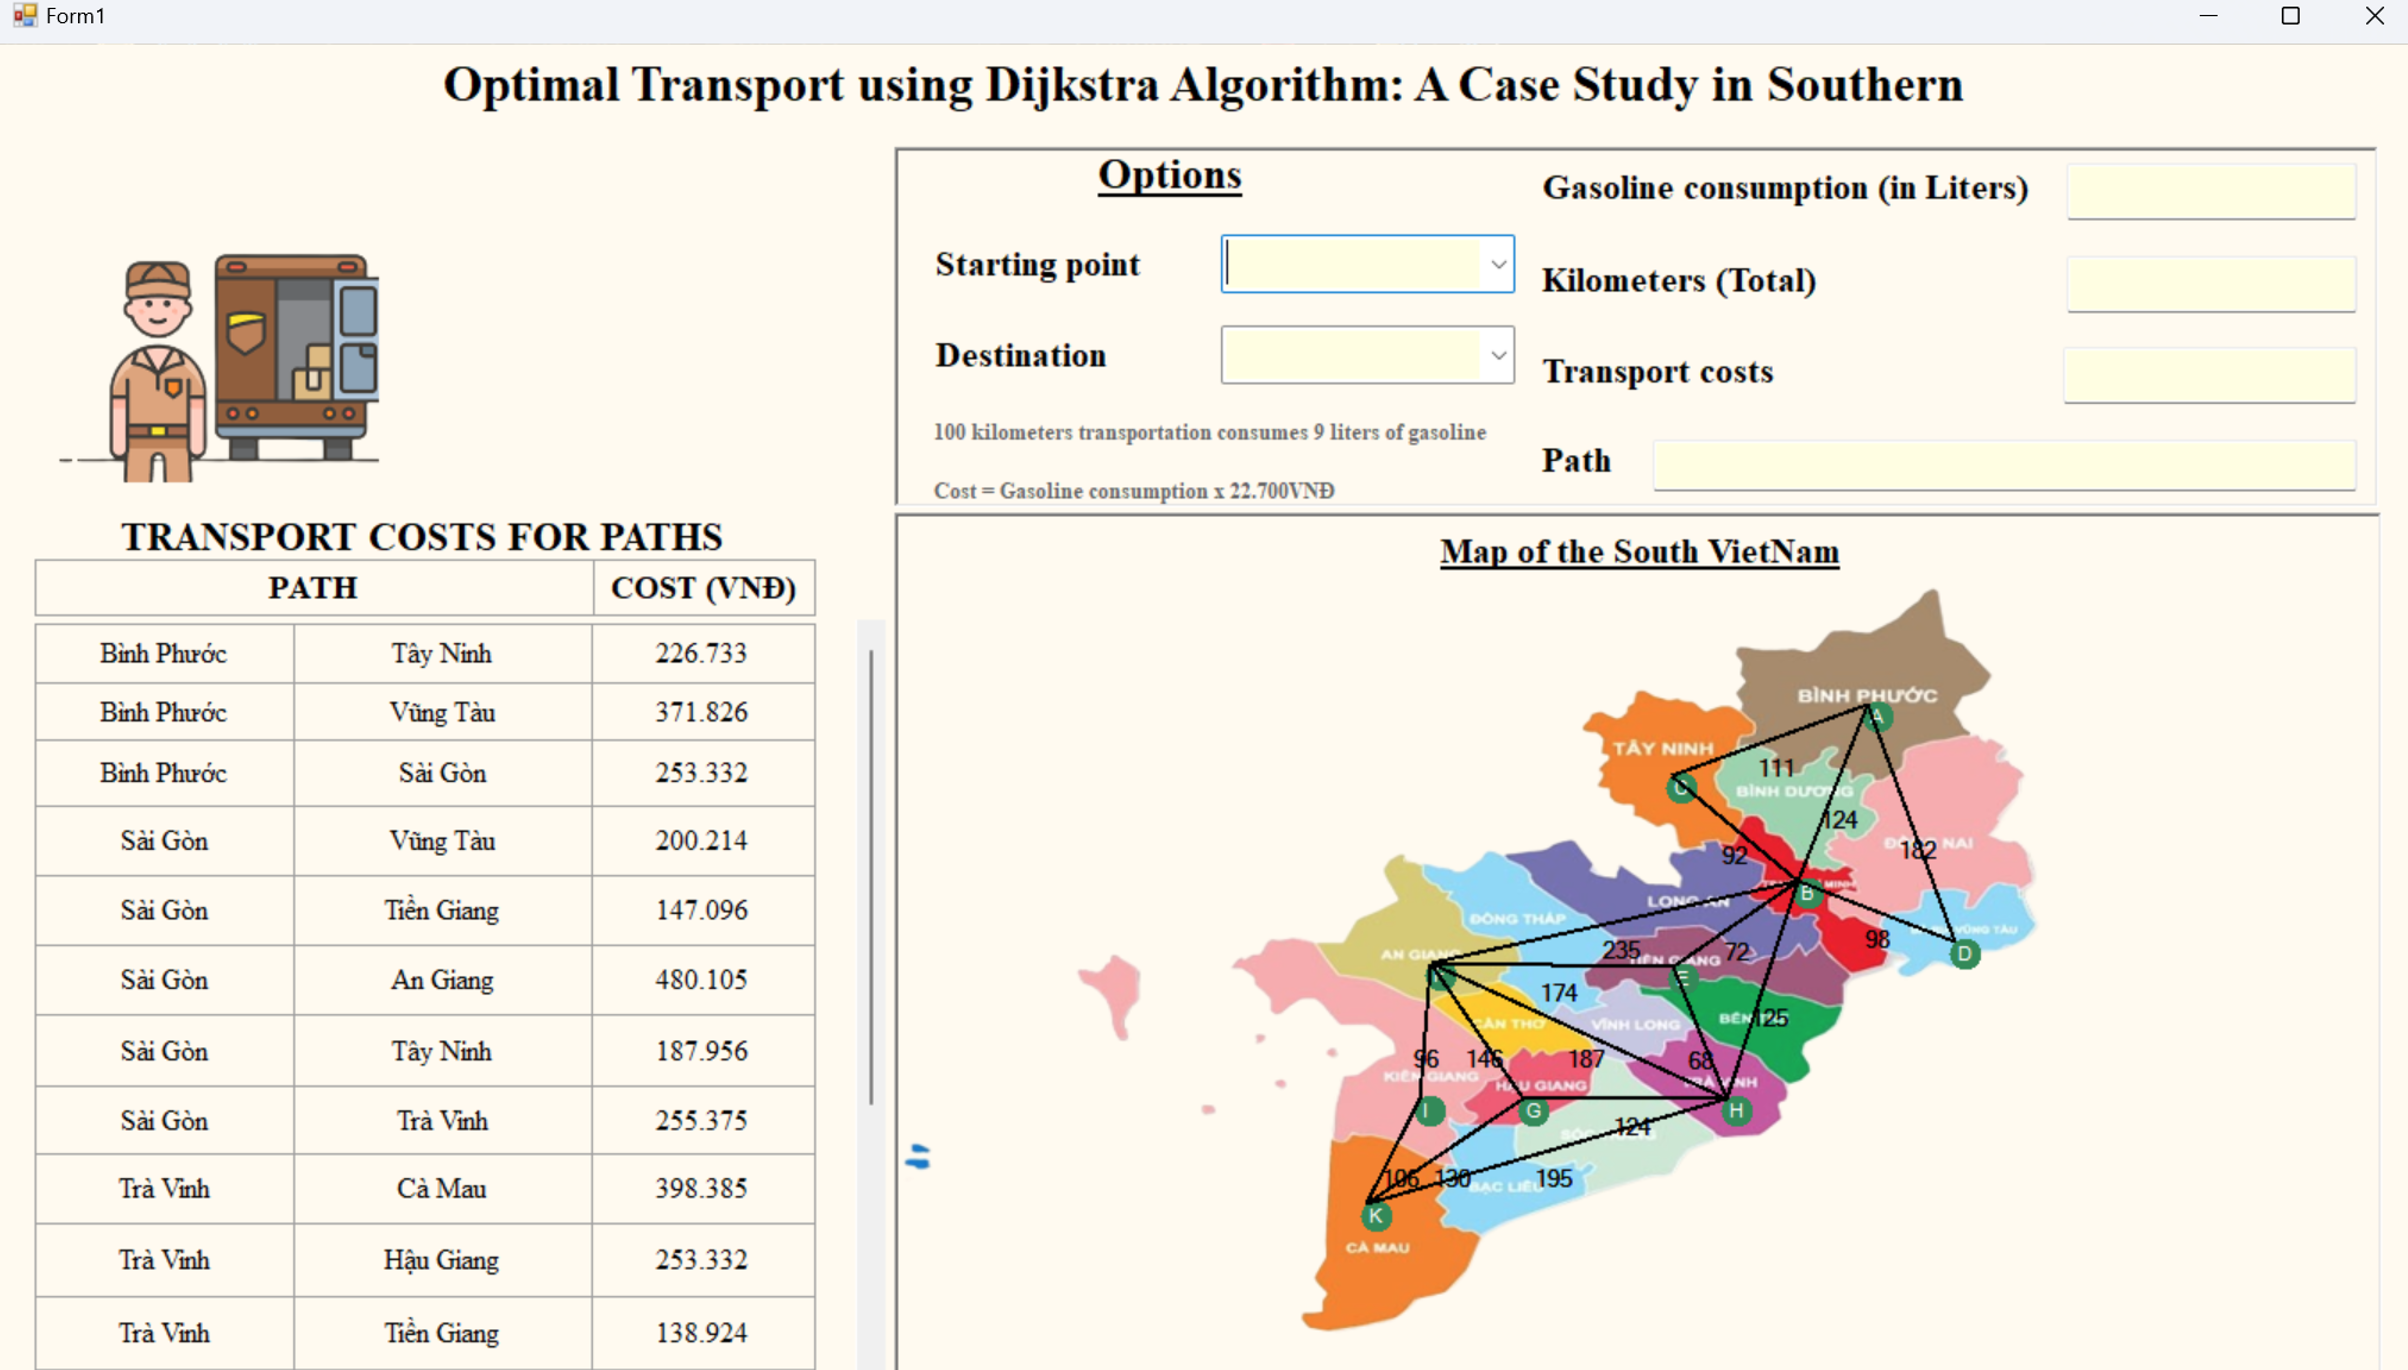
\includegraphics[width=17cm]{3.1.png}
    \caption{Giao diện menu chính}
\end{figure}
Mã nguồn chi tiết cấu tạo của giao diện có thể được tìm thấy tại phần \hyperref[appendix]{Phụ lục}
\subsection{Chi tiết chức năng}
\subsubsection{Bản đồ khu vực các tỉnh miền Nam Việt Nam và bảng giá vận chuyển}

\begin{itemize}
\begin{figure}[!ht]
    \centering
    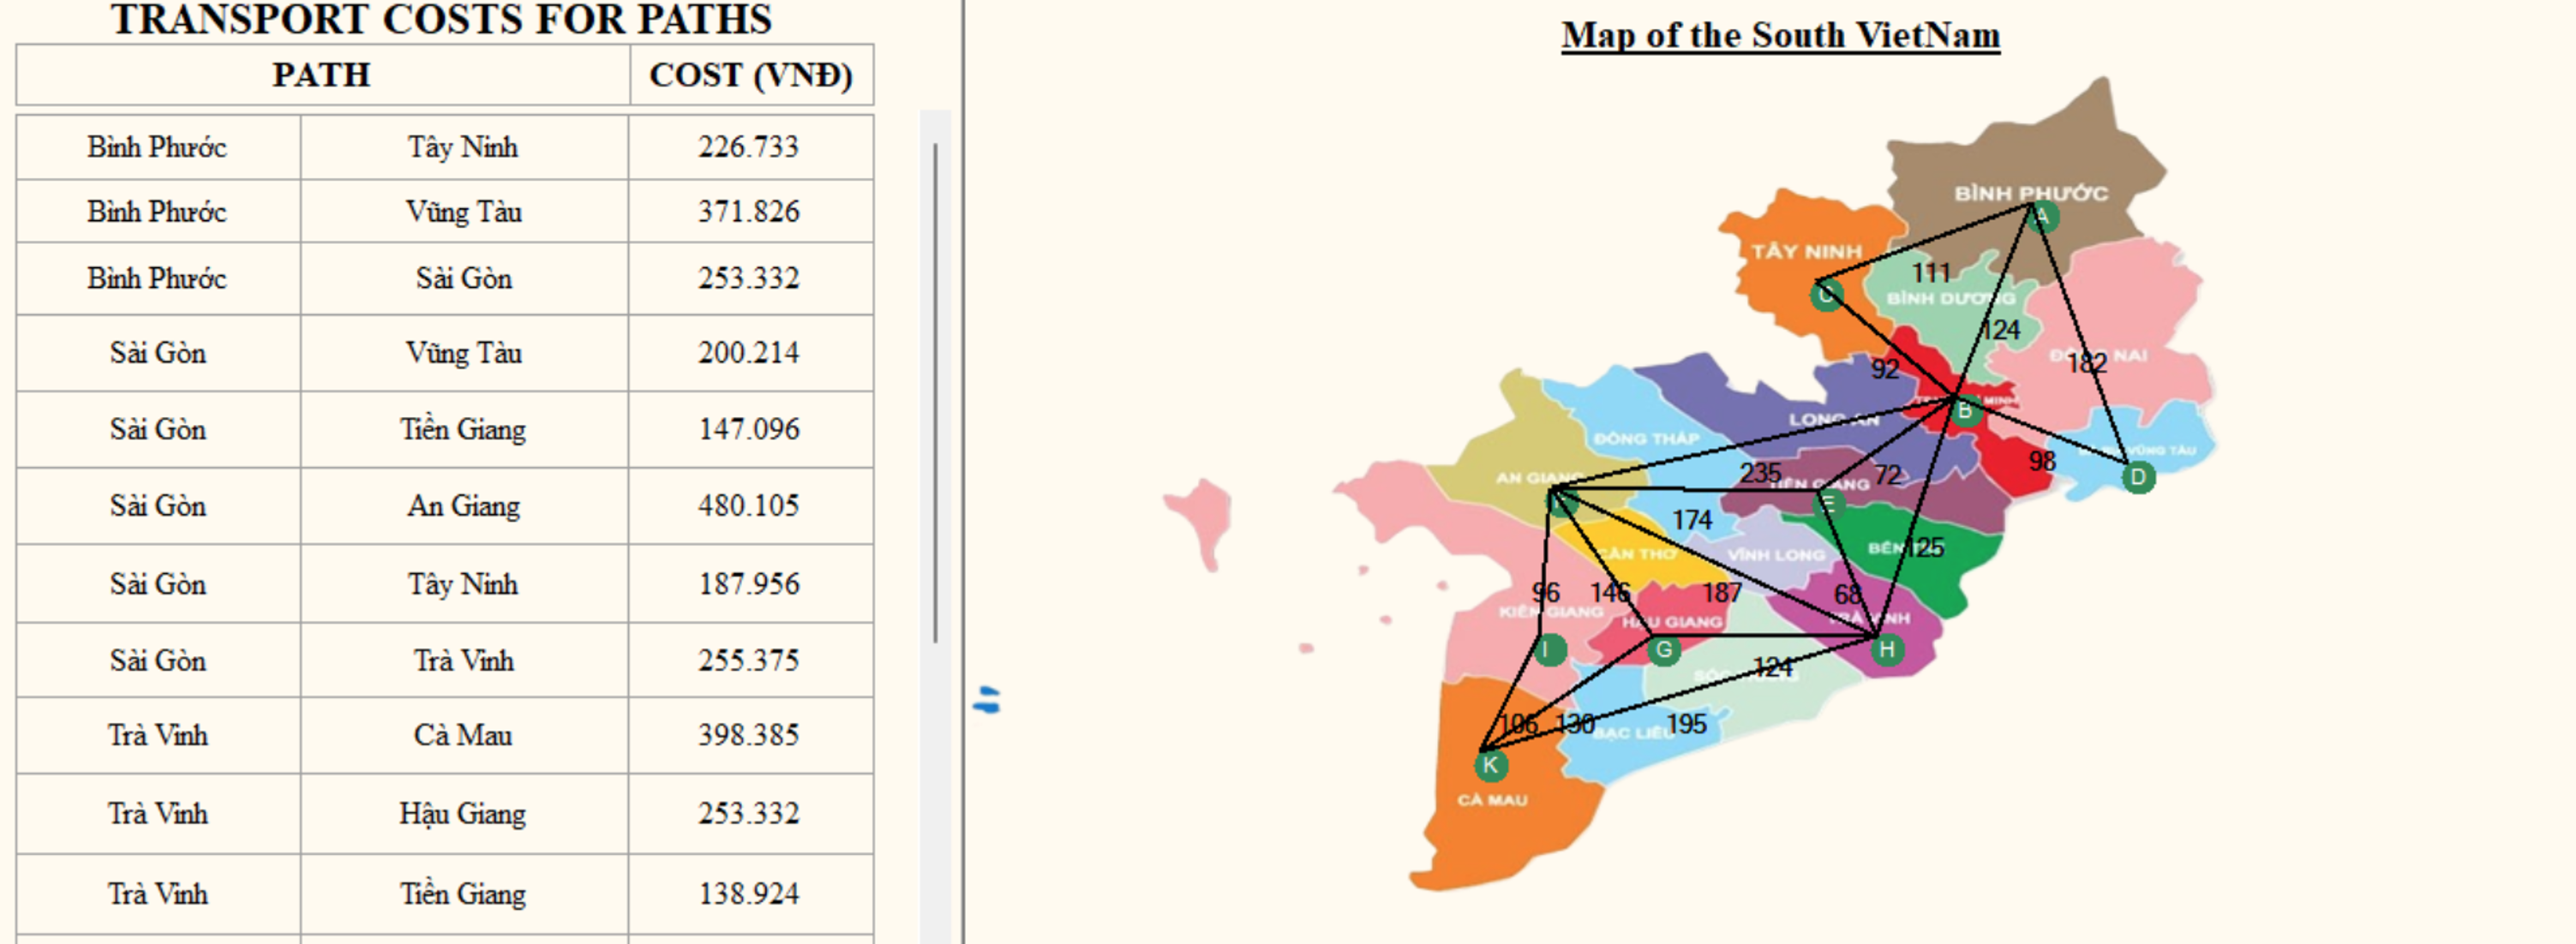
\includegraphics[width=17cm]{3.2.png}
    \caption{Bản đồ khu vực các tỉnh miền Nam Việt Nam và bảng giá vận chuyển}
\end{figure}
    \item Bản đồ hiển thị thông tin được đo đạc và liệt kê sẵn cho người dùng như: Những địa điểm vận chuyển, những tuyến đường, độ dài các tuyến đường.
    \item Bảng giá hiển thị chi phí vận chuyển giữa các tuyến đường, được hiển thị dưới dạng thanh cuộn.
\end{itemize}
\textbf{Mã nguồn các hàm chức năng:}
\begin{itemize}
    \item Hàm thêm các điểm và các tỉnh vào tọa độ theo bản đồ
\begin{minted}[tabsize=2,breaklines,frame=lines,framesep=2mm,baselinestretch=1.2,fontsize=\footnotesize, linenos]
{csharp}
public class Location
    {
        private string nameLocation { get; set; }
        private string pointName { get; set; }
        private Point pointLocation { get; set; }

        public Location(string name, string symbol, int x, int y)
        {
            nameLocation = name;
            pointName = symbol;
            Point p = new Point(x, y);
            pointLocation = p;
        }
        public string getName()
        {
            return nameLocation;
        }
        public string getPointName()
        {
            return pointName;
        }
        public Point getPoint()
        {
            return pointLocation;
        }
    }
public List<Location> Locations = new List<Location>();
SetUpGraph g = new SetUpGraph();
private void Form1_Load(object creator, EventArgs e)
{
     Location binhPhuoc = new Location("Bình Phước", "A", 541, 65);
     Location saiGon = new Location("Sài Gòn", "B", 502, 164);
     Location tayNinh = new Location("Tây Ninh", "C", 431, 105);
     Location vungTau = new Location("Vũng Tàu", "D", 590, 198);
     Location tienGiang = new Location("Tiền Giang", "E", 432, 212);
     Location anGiang = new Location("An Giang", "F", 296, 210);
     Location hauGiang = new Location("Hậu Giang", "G", 348, 286);
     Location traVinh = new Location("Trà Vinh", "H", 462, 286);
     Location kienGiang = new Location("Kiên Giang", "I", 290, 286);
     Location caMau = new Location("Cà Mau", "K", 260, 345);
\end{minted}

\item Hàm vẽ các điểm và nối các điểm thành các tuyến đường.
\begin{minted}[tabsize=2,breaklines,frame=lines,framesep=2mm,baselinestretch=1.2,fontsize=\footnotesize, linenos]
{csharp}
private void southMap_Paint(object creator, PaintEventArgs e)
{
     Graphics graph = southMap.CreateGraphics();
            for (int i = 0; i < Locations.Count; i++)
            {
                SolidBrush brush = new SolidBrush(Color.SeaGreen);
                Brush pointName = new SolidBrush(Color.White);
                graph.FillEllipse(brush, Locations[i].getPoint().X - 3, Locations[i].getPoint().Y - 2, 18, 18);
                graph.DrawString(Locations[i].getPointName(), new Font("Arial", 8), pointName, Locations[i].getPoint().X, Locations[i].getPoint().Y);
            }
            DrawLine();
        }

        private void DrawLine()
        {
            DrawLine("Tây Ninh", "Bình Phước");
            DrawLine("Vũng Tàu", "Bình Phước");
            DrawLine("Sài Gòn", "Bình Phước");
            DrawLine("Vũng Tàu", "Sài Gòn");
            DrawLine("Tiền Giang", "Sài Gòn");
            DrawLine("An Giang", "Sài Gòn");
            DrawLine("Tây Ninh", "Sài Gòn");
            DrawLine("Trà Vinh", "Sài Gòn");
            DrawLine("Trà Vinh", "Cà Mau");
            DrawLine("Trà Vinh", "Hậu Giang");
            DrawLine("Tiền Giang", "An Giang");
            DrawLine("Trà Vinh", "Tiền Giang");
            DrawLine("An Giang", "Trà Vinh");
            DrawLine("Hậu Giang", "Cà Mau");
            DrawLine("Cà Mau", "Kiên Giang");
            DrawLine("An Giang", "Hậu Giang");
            DrawLine("An Giang", "Kiên Giang");
        }
        private void DrawLine(string a, string b)
        {
            Graphics graph = southMap.CreateGraphics();
            int x = g.GetIndex(a);
            int y = g.GetIndex(b);
            Pen p = new Pen(Color.Black, 2);
            Point point1 = new Point(g.listPoint[x].X, g.listPoint[x].Y);
            Point point2 = new Point(g.listPoint[y].X, g.listPoint[y].Y);
            graph.DrawLine(p, point1, point2);
            graph.DrawString($"{g.adj[x, y]}", new Font("Fira Code", 10), Brushes.Black, new Point((point1.X + point2.X) / 2 - 8, (point1.Y + point2.Y) / 2 + 8));
        }
\end{minted}

\item Hàm thể hiện độ dài các tuyến đường
\begin{minted}[tabsize=2,breaklines,frame=lines,framesep=2mm,baselinestretch=1.2,fontsize=\footnotesize, linenos]
{csharp}
Graphics graph = southMap.CreateGraphics();
            for (int i = 0; i < Locations.Count; i++)
            {
                lvListProvinces.Items.Add(Locations[i].getPointName());
                lvListProvinces.Items[i].SubItems.Add(Locations[i].getName());
                g.listPoint.Add(Locations[i].getPoint());
                g.InsertVertex(Locations[i].getName());
            }
            g.InsertEdge("Tây Ninh", "Bình Phước", 111);
            g.InsertEdge("Vũng Tàu", "Bình Phước", 182);
            g.InsertEdge("Sài Gòn", "Bình Phước", 124);
            g.InsertEdge("Vũng Tàu", "Sài Gòn", 98);
            g.InsertEdge("Tiền Giang", "Sài Gòn", 72);
            g.InsertEdge("An Giang", "Sài Gòn", 235);
            g.InsertEdge("Tây Ninh", "Sài Gòn", 92);
            g.InsertEdge("Trà Vinh", "Sài Gòn", 125);
            g.InsertEdge("Trà Vinh", "Cà Mau", 195);
            g.InsertEdge("Trà Vinh", "Hậu Giang", 124);
            g.InsertEdge("Tiền Giang", "An Giang", 174);
            g.InsertEdge("Trà Vinh", "Tiền Giang", 68);
            g.InsertEdge("An Giang", "Trà Vinh", 187);
            g.InsertEdge("Hậu Giang", "Cà Mau", 130);
            g.InsertEdge("Cà Mau", "Kiên Giang", 106);
            g.InsertEdge("An Giang", "Hậu Giang", 146);
            g.InsertEdge("An Giang", "Kiên Giang", 96);
\end{minted}

\item Hàm vẽ tuyết đường tiết kiệm nhất tính toán được lên bản đồ
\begin{minted}[tabsize=2,breaklines,frame=lines,framesep=2mm,baselinestretch=1.2,fontsize=\footnotesize, linenos]
{csharp}
private void DrawPathLine(int i)
        {
            Graphics graph = southMap.CreateGraphics();
            Pen p = new Pen(Color.Aqua, 2);
            Point point1 = new Point(g.pathIndex[i].X, g.pathIndex[i].Y);
            Point point2 = new Point(g.pathIndex[i + 1].X, g.pathIndex[i + 1].Y);
            graph.DrawLine(p, point1, point2);
     }
\end{minted}
\end{itemize}
\subsubsection{Khung nhập và hiện thị kết quả}
\begin{figure}[!ht]
    \centering
    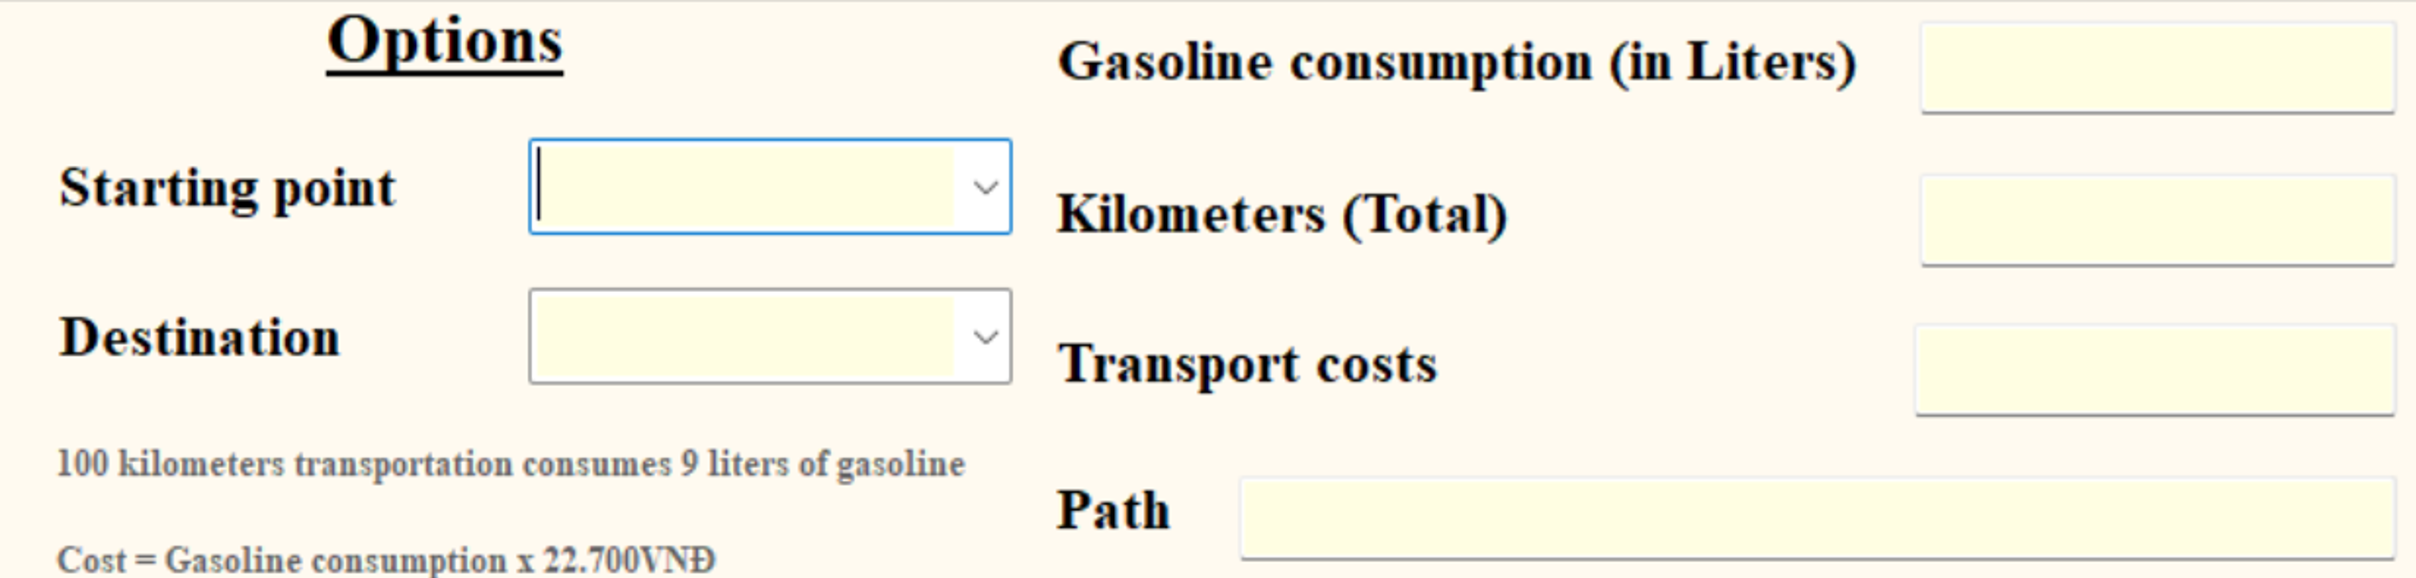
\includegraphics[width=17cm]{3.3.png}
    \caption{Khung nhập và hiện thị kết quả}
\end{figure}
Bảng này chia làm 2 phần, nhập đầu vào và hiện thị kết quả. Với đầu nhập vào thì sẽ nhập điểm đi và điểm đến, sau khi nhập vào chương trình sẽ tính toán và xuất ra các kết quả như : tổng số lít xăng cần để đi hết chặng đường, tổng độ dài, tổng chi phí và hiện ra tuyến đường tiết kiệm nhất.\\
(Thông tin đi kèm để người dùng hiểu các kết quả được hiển thị rằng 100 kilomet đi đường sẽ tiêu tốn 9 lít xăng, với giả sử rằng giá mỗi lít xăng là 22.700 VNĐ).\\
\textbf{Mã nguồn các hàm chức năng}
\begin{itemize}
    \item Hàm để thêm các thông tin vào input
    \begin{minted}[tabsize=2,breaklines,frame=lines,framesep=2mm,baselinestretch=1.2,fontsize=\footnotesize, linenos]
{csharp}
Locations.Add(binhPhuoc);
Locations.Add(saiGon);
Locations.Add(tayNinh);
Locations.Add(vungTau);
Locations.Add(tienGiang);
Locations.Add(anGiang);
Locations.Add(hauGiang);
Locations.Add(traVinh);
Locations.Add(kienGiang);
Locations.Add(caMau);
cbSource.Items.Add("Bình Phước");
cbSource.Items.Add("Sài Gòn");
cbSource.Items.Add("Tây Ninh");
cbSource.Items.Add("Vũng Tàu");
cbSource.Items.Add("Tiền Giang");
cbSource.Items.Add("An Giang");
cbSource.Items.Add("Hậu Giang");
cbSource.Items.Add("Trà Vinh");
cbSource.Items.Add("Kiên Giang");
cbSource.Items.Add("Cà Mau");
cbDestination.Items.Add("Bình Phước");
cbDestination.Items.Add("Sài Gòn");
cbDestination.Items.Add("Tây Ninh");
cbDestination.Items.Add("Vũng Tàu");
cbDestination.Items.Add("Tiền Giang");
cbDestination.Items.Add("An Giang");
cbDestination.Items.Add("Hậu Giang");
cbDestination.Items.Add("Trà Vinh");
cbDestination.Items.Add("Kiên Giang");
cbDestination.Items.Add("Cà Mau");
    \end{minted}
    
    \item Hàm để xuất các thông tin ra bảng màn hình.\\
    Trong đó
    \begin{itemize}
        \item \texttt{tbKM} hiển thị số kilomet tổng
        \item  \texttt{tbLiter} hiển thị số lít xăng ước tính
        \item \texttt{tbCost} hiển thị chi phí tổng
        \item \texttt{tbPath} hiến thị tuyến đường tiết kiệm nhất theo tính toán
    \end{itemize}
    \begin{minted}[tabsize=2,breaklines,frame=lines,framesep=2mm,baselinestretch=1.2,fontsize=\footnotesize, linenos]
{csharp}
public void FindPaths(string source, string last,TextBox tbKM,TextBox tbLiter, TextBox tbCost, TextBox tbPath)
{
    int s = GetIndex(source);
    Dijkstra(s);
    int v = Convert.ToInt32(last);
    {
        if (v != s)
        {
            if (vertexList[v].pathLength == INFINITY)
            {
                tbPath.Text += "\tNo path \n";
            }
            else
            {
                FindPath(s, v,tbKM, tbLiter, tbCost, tbPath);
            }
        }
    }
}
public void FindPath(int s, int v, TextBox tbKM, TextBox tbLiter, TextBox tbCost, TextBox tbPath)
{
    int i, u;
    int[] path = new int[n];
    int km = 0;
    int count = 0;
    while (v != s)
    {
        count++;
        path[count] = v;
        u = vertexList[v].predecessor;
        km += adj[u, v];
        v = u;
    }
    double sl = km * 0.09;
    int sd = km * 2043;
    count++;
    path[count] = s;
    for (i = count; i >= 1; i--)
    {
        pathIndex.Add(listPoint[path[i]]);
        if (tbPath.Text == "")
        {
            tbPath.Text += vertexList[path[i]].name;
        }
        else
        {
            tbPath.Text += " -> " + vertexList[path[i]].name;
        }
    }
    tbKM.Text = $"{km} KM";
    tbLiter.Text = $"{sl} liters";
    tbCost.Text = $"{sd} VNĐ";
     }
\end{minted}
        \item Hàm xóa các thông tin đã in ra từ trước khi nhập input khác và thông báo lỗi khi nhập trùng điểm đi và điểm đến
    \begin{minted}[tabsize=2,breaklines,frame=lines,framesep=2mm,baselinestretch=1.2,fontsize=\footnotesize, linenos]
{csharp}
private void cbSource_SelectedIndexChanged(object creator, EventArgs e)
        {
            if (cbSource.SelectedIndex != -1 && cbDestination.SelectedIndex != -1)
            {
                southMap.Controls.Clear();
                southMap.Refresh();
                DrawLine();
                g.pathIndex.Clear();
                tbKM.Clear();
                tbLiter.Clear();
                tbCost.Clear();
                tbPath.Clear();
                g.FindPaths(cbSource.SelectedItem.ToString(), cbDestination.SelectedIndex.ToString(),tbKM,tbLiter, tbCost, tbPath);
                for (int i = 0; i < g.pathIndex.Count - 1; i++)
                {
                    DrawPathLine(i);
                }
            }
            if (cbSource.SelectedIndex == cbDestination.SelectedIndex)
            {
                MessageBox.Show("Unresponsive\n The location can't be the same !", "Notify!");
            }
        }
        private void cbDestination_SelectedIndexChanged(object creator, EventArgs e)
        {
            if (cbSource.SelectedIndex != -1 && cbDestination.SelectedIndex != -1)
            {
                southMap.Controls.Clear();
                southMap.Refresh();
                DrawLine();
                g.pathIndex.Clear();
                tbKM.Clear();
                tbLiter.Clear();
                tbCost.Clear();
                tbPath.Clear();
                g.FindPaths(cbSource.SelectedItem.ToString(), cbDestination.SelectedIndex.ToString(),tbKM ,tbLiter, tbCost, tbPath);
                for (int i = 0; i < g.pathIndex.Count - 1; i++)
                {
                    DrawPathLine(i);
                }
            }
            if (cbSource.SelectedIndex == cbDestination.SelectedIndex)
            {
                MessageBox.Show("Unresponsive\n The location can't be the same !", "Notify!");
            }    
        }
    \end{minted}
\begin{figure}[!ht]
    \centering
    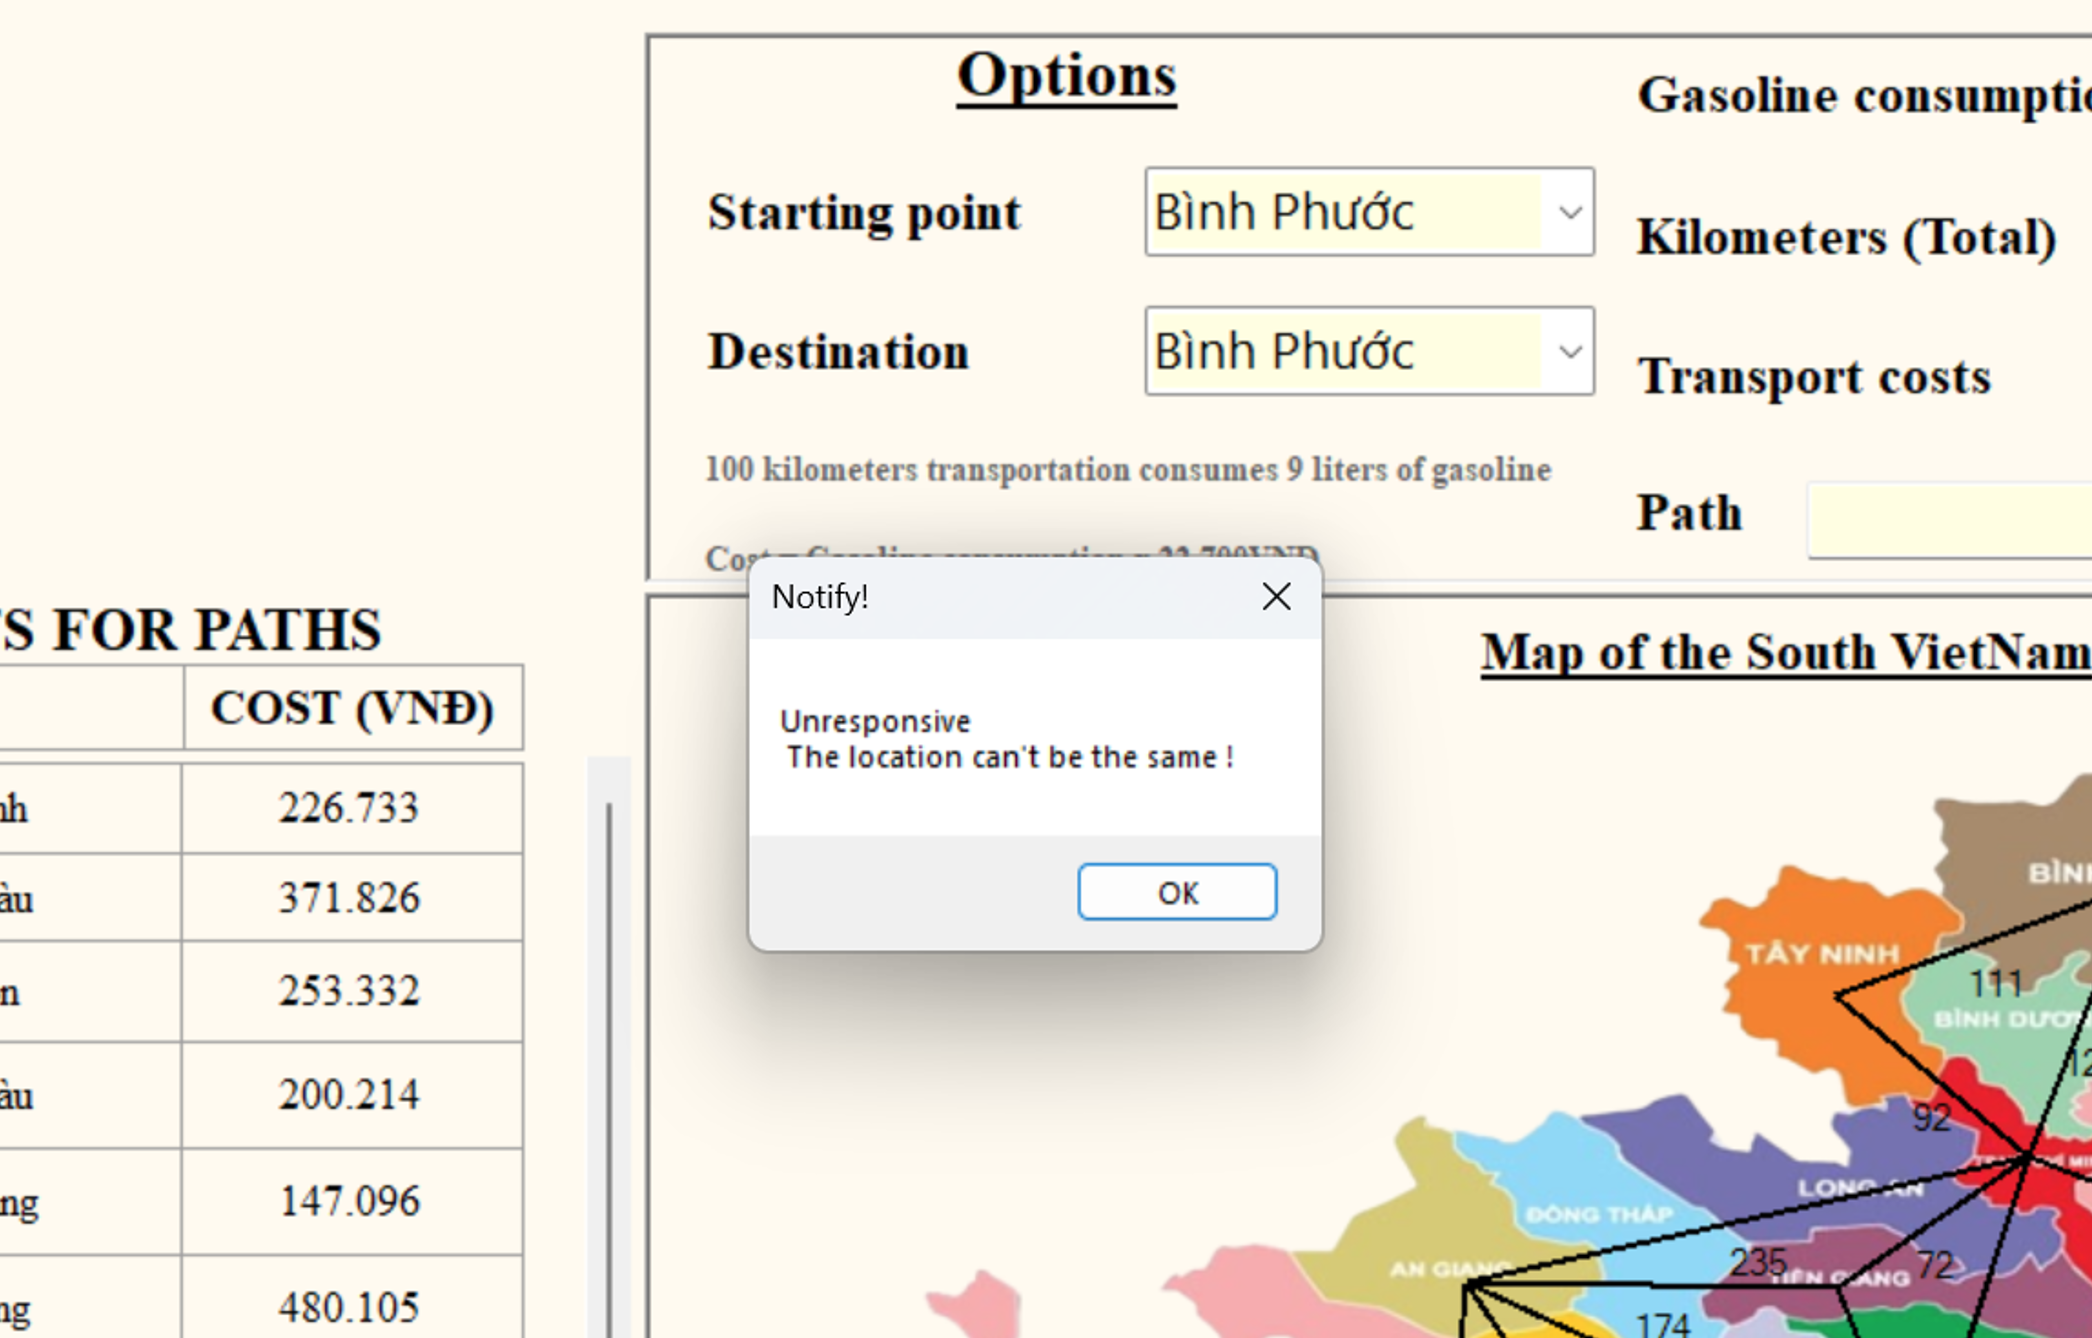
\includegraphics[width=17cm]{3.4.png}
    \caption{Chương trình hiện thông báo khi điểm đi trùng điểm đến}
\end{figure}
\end{itemize}

\subsubsection{Tổng kết các chức năng}
\begin{itemize}
\item Hiển thị bản đồ để người dùng dễ thao tác, trên bản đồ có các địa điểm và các tuyến đường đã được tính trước độ dài.
\item Có bảng chi phí giữa các tuyến đường được tính ra dựa trên độ dài các địa điểm
\item Có ô nhập các điểm đi và điểm đến dựa trên các thông tin có sẵn.
\item Có ô hiển thị các thông tin cần thiết cho người dùng như số lít xăng, số kilomet tổng thể, chi phí cần bỏ ra và tuyến đường hợp lý nhất.
\item Vẽ tuyến đường ngắn nhất lên bản đồ và sau khi hiện tuyến đường khác thì xóa đi và vẽ đường mới.
\item Thông báo khi nhập trùng điểm.
\end{itemize}
\section{Thảo luận và đánh giá}
Ứng dụng tối ưu tuyến đường giúp tìm được những quãng đường hiệu quả nhất giữa các điểm mà vẫn đáp ứng đủ yêu cầu được đưa vào bởi doanh nghiệp. Hơn nữa, ứng dụng còn giúp tiết dự đoán về cả thời gian, quãng đường và nhiên liệu hay các chi phí dự kiến phát sinh trong quá trình vận chuyển, giúp quá trình giao nhận hàng của các đội xe trở nên hiệu quả hơn bao giờ hết.
Hơn nữa, ứng dụng tối ưu tuyến đường còn có thể xử lý các chuyến đi tới nhiều địa điểm bằng cách thao tác địa điểm muốn đến từ địa điểm này đến địa điểm khác thông qua các dữ liệu tọa độ từ đó tìm ra tuyến đường ngắn nhất để đạt được nhiều hiệu quả, tiết kiệm nhiên liệu, tối thiểu hao mòn xe. Những yếu tố này sẽ giúp tiết kiệm chi phí phát sinh trong quá trình vận chuyển, giúp toàn bộ quá trình nhận và trả hàng hiệu quả hơn bao giờ hết.
\subsection{Một số tồn tại}
\subsubsection{Các chức năng chính}
\begin{itemize}
    \item Thanh cuộn ở bảng giá tiền vận chuyển từng tỉnh A qua từng tỉnh X
    \item Lựa chọn địa điểm xuất phát
    \item Lựa chọn địa điểm kết thúc
    \item Hiển thị tổng nhiên liệu nhiên liệu dự kiến tiêu thụ trong suốt quãng đường
    \item Hiển thị tổng km dự kiến trong tuyến đường
    \item Tính tổng chi phí vận tải đã được tối thiểu
    \item Hiển thị Popup thông báo lỗi
    \item Tuyến đường được thể hiện trực tiếp trên bản đồ
\end{itemize}
\subsubsection{Hạn chế}
Ứng dụng tìm kiếm chưa được tối ưu khi không thể hiện đầy đủ tất cả thông tin liên quan đến ảnh hưởng chi phí vận tải:
\begin{itemize}
\item Không thể hiện chi tiết quãng đường cụ thể
\item Chưa cập nhật các yếu tố thời gian thực như tắc nghẽn giao thông,  ảnh hưởng của thời tiết, điều kiện đường đi, giá xăng
\item Việc tìm kiếm quãng đường đi xảy ra mâu thuẫn do chưa đa dạng phương tiện vận tải
\end{itemize}
\subsection{Hướng phát triển}
\textbf{Tạo bản đồ cụ thể địa điểm:}
\begin{itemize}
\item Địa điểm xuất phát, địa điểm đến cần mô phỏng chi tiết hơn tại vị trí nào của địa điểm đó
\item Có thông tin về địa điểm xuất phát hoặc đến một cách chi tiết liên quan đến việc ảnh hưởng chi phí vận tải 
\item Đổi mới màu sắc đường đi cũng như là bản đồ cho phù hợp 
\item Thêm các đỉnh tạo nên các địa điểm mới trên bản đồ
\item Thêm các cạnh giữa các các đỉnh để tạo thêm đường đi qua các tỉnh trên bản đồ
\end{itemize}
\textbf{Đa phương tiện vận tải:}
\begin{itemize}
\item Ngoài phương tiện trên đường bộ thì cần phát triển hệ thống các phương tiện trên cả đường thuỷ, đường hàng không và bao gồm cả đường sắt  
\item Thêm chức năng chọn phương tiện vận tải kèm với tải trọng phù hợp để tiết kiệm chi nhất có thể
\item Thêm các tuyến đường dành cho phương tiện phù hợp nêu trên
\item Ngoài ra, cần thêm chức năng tính toán thời gian dự kiến hàng hoá sẽ được vận chuyển từ tỉnh A sang tỉnh X cho từng phương tiện vận tải để có thể tối ứu hoá về cả thời gian và chi phí. 
\end{itemize}
\textbf{Thêm thông tin ảnh hưởng chi phí vận tải trên bản đồ:}
\begin{itemize}
\item Cập nhật thời tiết theo thời gian
\item Cập nhật giá xăng dầu qua từng ngày
\item Cập nhật màu sắc đường đi trên đoạn đường ùn tắc
\item Cập nhật số lượng trạm thu phí trên suốt đường đi
\end{itemize}
\section{Phụ lục} \label{appendix}
\subsection{Mã nguồn Github}
Toàn bộ mã nguồn có thể được tìm thấy tại \underline{\textbf{\href{https://github.com/quocviethere/DSA-Project-Dijkstra-Algorithm}{Link GitHub}}}
\subsection{Chi tiết mã nguồn cấu tạo giao diện}
\begin{minted}[tabsize=2,breaklines,frame=lines,framesep=2mm,baselinestretch=1.2,fontsize=\footnotesize, linenos]
{csharp}
namespace DijkstraTest2
{
    partial class Form1
    {
        /// <summary>
        /// Required designer variable.
        /// </summary>
        private System.ComponentModel.IContainer components = null;

        /// <summary>
        /// Clean up any resources being used.
        /// </summary>
        /// <param name="disposing">true if managed resources should be disposed; otherwise, false.</param>
        protected override void Dispose(bool disposing)
        {
            if (disposing && (components != null))
            {
                components.Dispose();
            }
            base.Dispose(disposing);
        }

        #region Windows Form Designer generated code

        /// <summary>
        /// Required method for Designer support - do not modify
        /// the contents of this method with the code editor.
        /// </summary>
        private void InitializeComponent()
        {
            this.lbInfo = new System.Windows.Forms.Label();
            this.label3 = new System.Windows.Forms.Label();
            this.label5 = new System.Windows.Forms.Label();
            this.label6 = new System.Windows.Forms.Label();
            this.label1 = new System.Windows.Forms.Label();
            this.lvListProvinces = new System.Windows.Forms.ListView();
            this.clPoint = ((System.Windows.Forms.ColumnHeader)(new System.Windows.Forms.ColumnHeader()));
            this.clName = ((System.Windows.Forms.ColumnHeader)(new System.Windows.Forms.ColumnHeader()));
            this.flowLayoutPanel4 = new System.Windows.Forms.FlowLayoutPanel();
            this.label2 = new System.Windows.Forms.Label();
            this.southMap = new System.Windows.Forms.PictureBox();
            this.cbSource = new System.Windows.Forms.ComboBox();
            this.cbDestination = new System.Windows.Forms.ComboBox();
            this.panel3 = new System.Windows.Forms.Panel();
            this.tbPath = new System.Windows.Forms.TextBox();
            this.tbKM = new System.Windows.Forms.TextBox();
            this.label7 = new System.Windows.Forms.Label();
            this.lable12 = new System.Windows.Forms.Label();
            this.tbLiter = new System.Windows.Forms.TextBox();
            this.tbCost = new System.Windows.Forms.TextBox();
            this.label8 = new System.Windows.Forms.Label();
            this.label9 = new System.Windows.Forms.Label();
            this.pictureBox1 = new System.Windows.Forms.PictureBox();
            this.tableLayoutPanel1 = new System.Windows.Forms.TableLayoutPanel();
            this.label45 = new System.Windows.Forms.Label();
            this.label11 = new System.Windows.Forms.Label();
            this.label14 = new System.Windows.Forms.Label();
            this.label15 = new System.Windows.Forms.Label();
            this.label13 = new System.Windows.Forms.Label();
            this.label16 = new System.Windows.Forms.Label();
            this.label17 = new System.Windows.Forms.Label();
            this.label18 = new System.Windows.Forms.Label();
            this.label19 = new System.Windows.Forms.Label();
            this.label20 = new System.Windows.Forms.Label();
            this.label21 = new System.Windows.Forms.Label();
            this.label22 = new System.Windows.Forms.Label();
            this.label23 = new System.Windows.Forms.Label();
            this.label24 = new System.Windows.Forms.Label();
            this.label25 = new System.Windows.Forms.Label();
            this.label26 = new System.Windows.Forms.Label();
            this.label27 = new System.Windows.Forms.Label();
            this.label28 = new System.Windows.Forms.Label();
            this.label29 = new System.Windows.Forms.Label();
            this.label30 = new System.Windows.Forms.Label();
            this.label31 = new System.Windows.Forms.Label();
            this.label32 = new System.Windows.Forms.Label();
            this.label33 = new System.Windows.Forms.Label();
            this.label34 = new System.Windows.Forms.Label();
            this.label35 = new System.Windows.Forms.Label();
            this.label36 = new System.Windows.Forms.Label();
            this.label37 = new System.Windows.Forms.Label();
            this.label38 = new System.Windows.Forms.Label();
            this.label39 = new System.Windows.Forms.Label();
            this.label40 = new System.Windows.Forms.Label();
            this.label41 = new System.Windows.Forms.Label();
            this.label42 = new System.Windows.Forms.Label();
            this.label43 = new System.Windows.Forms.Label();
            this.label44 = new System.Windows.Forms.Label();
            this.label46 = new System.Windows.Forms.Label();
            this.label47 = new System.Windows.Forms.Label();
            this.label48 = new System.Windows.Forms.Label();
            this.label49 = new System.Windows.Forms.Label();
            this.label50 = new System.Windows.Forms.Label();
            this.label51 = new System.Windows.Forms.Label();
            this.label52 = new System.Windows.Forms.Label();
            this.label53 = new System.Windows.Forms.Label();
            this.label54 = new System.Windows.Forms.Label();
            this.label55 = new System.Windows.Forms.Label();
            this.label56 = new System.Windows.Forms.Label();
            this.label57 = new System.Windows.Forms.Label();
            this.label58 = new System.Windows.Forms.Label();
            this.label59 = new System.Windows.Forms.Label();
            this.label60 = new System.Windows.Forms.Label();
            this.label61 = new System.Windows.Forms.Label();
            this.label62 = new System.Windows.Forms.Label();
            this.label64 = new System.Windows.Forms.Label();
            this.flowLayoutPanel1 = new System.Windows.Forms.FlowLayoutPanel();
            this.tableLayoutPanel2 = new System.Windows.Forms.TableLayoutPanel();
            this.label4 = new System.Windows.Forms.Label();
            this.label10 = new System.Windows.Forms.Label();
            this.flowLayoutPanel4.SuspendLayout();
            ((System.ComponentModel.ISupportInitialize)(this.southMap)).BeginInit();
            this.panel3.SuspendLayout();
            ((System.ComponentModel.ISupportInitialize)(this.pictureBox1)).BeginInit();
            this.tableLayoutPanel1.SuspendLayout();
            this.flowLayoutPanel1.SuspendLayout();
            this.tableLayoutPanel2.SuspendLayout();
            this.SuspendLayout();
            // 
            // lbInfo
            // 
            this.lbInfo.AutoSize = true;
            this.lbInfo.Font = new System.Drawing.Font("Times New Roman", 21F, System.Drawing.FontStyle.Bold, System.Drawing.GraphicsUnit.Point, ((byte)(0)));
            this.lbInfo.Location = new System.Drawing.Point(423, 36);
            this.lbInfo.Margin = new System.Windows.Forms.Padding(4, 0, 4, 0);
            this.lbInfo.Name = "lbInfo";
            this.lbInfo.Size = new System.Drawing.Size(1312, 48);
            this.lbInfo.TabIndex = 1;
            this.lbInfo.Text = "Optimal Transport using Dijkstra Algorithm: A Case Study in Southern ";
            // 
            // label3
            // 
            this.label3.Font = new System.Drawing.Font("Times New Roman", 18F, ((System.Drawing.FontStyle)((System.Drawing.FontStyle.Bold | System.Drawing.FontStyle.Underline))), System.Drawing.GraphicsUnit.Point, ((byte)(0)));
            this.label3.Location = new System.Drawing.Point(147, 0);
            this.label3.Margin = new System.Windows.Forms.Padding(4, 0, 4, 0);
            this.label3.Name = "label3";
            this.label3.Size = new System.Drawing.Size(166, 75);
            this.label3.TabIndex = 3;
            this.label3.Text = "Options";
            this.label3.TextAlign = System.Drawing.ContentAlignment.TopCenter;
            // 
            // label5
            // 
            this.label5.Font = new System.Drawing.Font("Times New Roman", 15F, System.Drawing.FontStyle.Bold, System.Drawing.GraphicsUnit.Point, ((byte)(0)));
            this.label5.Location = new System.Drawing.Point(25, 80);
            this.label5.Margin = new System.Windows.Forms.Padding(4, 0, 4, 0);
            this.label5.Name = "label5";
            this.label5.Size = new System.Drawing.Size(288, 69);
            this.label5.TabIndex = 4;
            this.label5.Text = "Starting point";
            // 
            // label6
            // 
            this.label6.Font = new System.Drawing.Font("Times New Roman", 15F, System.Drawing.FontStyle.Bold, System.Drawing.GraphicsUnit.Point, ((byte)(0)));
            this.label6.Location = new System.Drawing.Point(25, 220);
            this.label6.Margin = new System.Windows.Forms.Padding(4, 0, 4, 0);
            this.label6.Name = "label6";
            this.label6.Size = new System.Drawing.Size(288, 69);
            this.label6.TabIndex = 5;
            this.label6.Text = "Destination";
            // 
            // label1
            // 
            this.label1.Font = new System.Drawing.Font("Comic Sans MS", 14.25F, ((System.Drawing.FontStyle)((System.Drawing.FontStyle.Bold | System.Drawing.FontStyle.Underline))), System.Drawing.GraphicsUnit.Point, ((byte)(0)));
            this.label1.Location = new System.Drawing.Point(4, 0);
            this.label1.Margin = new System.Windows.Forms.Padding(4, 0, 4, 0);
            this.label1.Name = "label1";
            this.label1.Size = new System.Drawing.Size(964, 58);
            this.label1.TabIndex = 2;
            this.label1.Text = "List of Provinces/Cities in South Vietnam";
            this.label1.TextAlign = System.Drawing.ContentAlignment.MiddleCenter;
            // 
            // lvListProvinces
            // 
            this.lvListProvinces.Columns.AddRange(new System.Windows.Forms.ColumnHeader[] {
            this.clPoint,
            this.clName});
            this.lvListProvinces.Font = new System.Drawing.Font("Comic Sans MS", 14.25F, System.Drawing.FontStyle.Bold, System.Drawing.GraphicsUnit.Point, ((byte)(0)));
            this.lvListProvinces.GridLines = true;
            this.lvListProvinces.HideSelection = false;
            this.lvListProvinces.Location = new System.Drawing.Point(4, 63);
            this.lvListProvinces.Margin = new System.Windows.Forms.Padding(4, 5, 4, 5);
            this.lvListProvinces.Name = "lvListProvinces";
            this.lvListProvinces.Size = new System.Drawing.Size(960, 656);
            this.lvListProvinces.TabIndex = 3;
            this.lvListProvinces.UseCompatibleStateImageBehavior = false;
            this.lvListProvinces.View = System.Windows.Forms.View.Details;
            // 
            // clPoint
            // 
            this.clPoint.Text = "Point";
            this.clPoint.Width = 235;
            // 
            // clName
            // 
            this.clName.Text = "Name";
            this.clName.TextAlign = System.Windows.Forms.HorizontalAlignment.Center;
            this.clName.Width = 400;
            // 
            // flowLayoutPanel4
            // 
            this.flowLayoutPanel4.BackColor = System.Drawing.Color.FloralWhite;
            this.flowLayoutPanel4.BorderStyle = System.Windows.Forms.BorderStyle.Fixed3D;
            this.flowLayoutPanel4.Controls.Add(this.label2);
            this.flowLayoutPanel4.Controls.Add(this.southMap);
            this.flowLayoutPanel4.Location = new System.Drawing.Point(754, 404);
            this.flowLayoutPanel4.Margin = new System.Windows.Forms.Padding(4, 5, 4, 5);
            this.flowLayoutPanel4.Name = "flowLayoutPanel4";
            this.flowLayoutPanel4.Size = new System.Drawing.Size(1249, 751);
            this.flowLayoutPanel4.TabIndex = 6;
            // 
            // label2
            // 
            this.label2.Font = new System.Drawing.Font("Times New Roman", 15F, ((System.Drawing.FontStyle)((System.Drawing.FontStyle.Bold | System.Drawing.FontStyle.Underline))), System.Drawing.GraphicsUnit.Point, ((byte)(0)));
            this.label2.Location = new System.Drawing.Point(4, 0);
            this.label2.Margin = new System.Windows.Forms.Padding(4, 0, 4, 0);
            this.label2.Name = "label2";
            this.label2.Size = new System.Drawing.Size(916, 58);
            this.label2.TabIndex = 2;
            this.label2.Text = "Map of the South VietNam";
            this.label2.TextAlign = System.Drawing.ContentAlignment.MiddleCenter;
            // 
            // southMap
            // 
            this.southMap.BackgroundImage = global::DijkstraTest2.Properties.Resources._1324532_removebg;
            this.southMap.BackgroundImageLayout = System.Windows.Forms.ImageLayout.Stretch;
            this.southMap.Image = global::DijkstraTest2.Properties.Resources._04142915_ban_do_cac_tinh_mien_nam_removebg__1_;
            this.southMap.Location = new System.Drawing.Point(3, 61);
            this.southMap.Name = "southMap";
            this.southMap.Size = new System.Drawing.Size(643, 423);
            this.southMap.SizeMode = System.Windows.Forms.PictureBoxSizeMode.AutoSize;
            this.southMap.TabIndex = 3;
            this.southMap.TabStop = false;
            this.southMap.Paint += new System.Windows.Forms.PaintEventHandler(this.southMap_Paint);
            // 
            // cbSource
            // 
            this.cbSource.BackColor = System.Drawing.SystemColors.Info;
            this.cbSource.Font = new System.Drawing.Font("Segoe UI", 14.25F, System.Drawing.FontStyle.Regular, System.Drawing.GraphicsUnit.Point, ((byte)(0)));
            this.cbSource.FormattingEnabled = true;
            this.cbSource.Location = new System.Drawing.Point(241, 73);
            this.cbSource.Margin = new System.Windows.Forms.Padding(4, 5, 4, 5);
            this.cbSource.Name = "cbSource";
            this.cbSource.Size = new System.Drawing.Size(231, 48);
            this.cbSource.TabIndex = 1;
            this.cbSource.SelectedIndexChanged += new System.EventHandler(this.cbSource_SelectedIndexChanged);
            // 
            // cbDestination
            // 
            this.cbDestination.BackColor = System.Drawing.SystemColors.Info;
            this.cbDestination.Font = new System.Drawing.Font("Segoe UI", 14.25F, System.Drawing.FontStyle.Regular, System.Drawing.GraphicsUnit.Point, ((byte)(0)));
            this.cbDestination.FormattingEnabled = true;
            this.cbDestination.Location = new System.Drawing.Point(241, 213);
            this.cbDestination.Margin = new System.Windows.Forms.Padding(4, 5, 4, 5);
            this.cbDestination.Name = "cbDestination";
            this.cbDestination.Size = new System.Drawing.Size(231, 48);
            this.cbDestination.TabIndex = 7;
            this.cbDestination.SelectedIndexChanged += new System.EventHandler(this.cbDestination_SelectedIndexChanged);
            // 
            // panel3
            // 
            this.panel3.BackColor = System.Drawing.Color.FloralWhite;
            this.panel3.BorderStyle = System.Windows.Forms.BorderStyle.Fixed3D;
            this.panel3.Controls.Add(this.cbSource);
            this.panel3.Controls.Add(this.label5);
            this.panel3.Controls.Add(this.cbDestination);
            this.panel3.Controls.Add(this.label6);
            this.panel3.Controls.Add(this.tbPath);
            this.panel3.Controls.Add(this.label3);
            this.panel3.Controls.Add(this.tbKM);
            this.panel3.Controls.Add(this.label7);
            this.panel3.Controls.Add(this.lable12);
            this.panel3.Controls.Add(this.tbLiter);
            this.panel3.Controls.Add(this.tbCost);
            this.panel3.Controls.Add(this.label8);
            this.panel3.Controls.Add(this.label9);
            this.panel3.Location = new System.Drawing.Point(754, 89);
            this.panel3.Margin = new System.Windows.Forms.Padding(4, 5, 4, 5);
            this.panel3.Name = "panel3";
            this.panel3.Size = new System.Drawing.Size(1246, 309);
            this.panel3.TabIndex = 10;
            // 
            // tbPath
            // 
            this.tbPath.BackColor = System.Drawing.SystemColors.Info;
            this.tbPath.Font = new System.Drawing.Font("Times New Roman", 14F, System.Drawing.FontStyle.Regular, System.Drawing.GraphicsUnit.Point, ((byte)(0)));
            this.tbPath.Location = new System.Drawing.Point(635, 263);
            this.tbPath.Margin = new System.Windows.Forms.Padding(4, 5, 4, 5);
            this.tbPath.Name = "tbPath";
            this.tbPath.Size = new System.Drawing.Size(690, 40);
            this.tbPath.TabIndex = 8;
            // 
            // tbKM
            // 
            this.tbKM.BackColor = System.Drawing.SystemColors.Info;
            this.tbKM.Font = new System.Drawing.Font("Times New Roman", 16F, System.Drawing.FontStyle.Regular, System.Drawing.GraphicsUnit.Point, ((byte)(0)));
            this.tbKM.Location = new System.Drawing.Point(983, 105);
            this.tbKM.Margin = new System.Windows.Forms.Padding(4, 5, 4, 5);
            this.tbKM.Name = "tbKM";
            this.tbKM.Size = new System.Drawing.Size(345, 44);
            this.tbKM.TabIndex = 11;
            // 
            // label7
            // 
            this.label7.Font = new System.Drawing.Font("Times New Roman", 15F, System.Drawing.FontStyle.Bold, System.Drawing.GraphicsUnit.Point, ((byte)(0)));
            this.label7.Location = new System.Drawing.Point(536, 188);
            this.label7.Margin = new System.Windows.Forms.Padding(4, 0, 4, 0);
            this.label7.Name = "label7";
            this.label7.Size = new System.Drawing.Size(242, 69);
            this.label7.TabIndex = 5;
            this.label7.Text = "Transport costs";
            // 
            // lable12
            // 
            this.lable12.Font = new System.Drawing.Font("Times New Roman", 15F, System.Drawing.FontStyle.Bold, System.Drawing.GraphicsUnit.Point, ((byte)(0)));
            this.lable12.Location = new System.Drawing.Point(536, 108);
            this.lable12.Margin = new System.Windows.Forms.Padding(4, 0, 4, 0);
            this.lable12.Name = "lable12";
            this.lable12.Size = new System.Drawing.Size(403, 69);
            this.lable12.TabIndex = 10;
            this.lable12.Text = "Kilometers (Total)";
            // 
            // tbLiter
            // 
            this.tbLiter.BackColor = System.Drawing.SystemColors.Info;
            this.tbLiter.Font = new System.Drawing.Font("Times New Roman", 16F, System.Drawing.FontStyle.Regular, System.Drawing.GraphicsUnit.Point, ((byte)(0)));
            this.tbLiter.Location = new System.Drawing.Point(983, 31);
            this.tbLiter.Margin = new System.Windows.Forms.Padding(4, 5, 4, 5);
            this.tbLiter.Name = "tbLiter";
            this.tbLiter.Size = new System.Drawing.Size(345, 44);
            this.tbLiter.TabIndex = 9;
            // 
            // tbCost
            // 
            this.tbCost.BackColor = System.Drawing.SystemColors.Info;
            this.tbCost.Font = new System.Drawing.Font("Times New Roman", 16F, System.Drawing.FontStyle.Regular, System.Drawing.GraphicsUnit.Point, ((byte)(0)));
            this.tbCost.Location = new System.Drawing.Point(980, 185);
            this.tbCost.Margin = new System.Windows.Forms.Padding(4, 5, 4, 5);
            this.tbCost.Name = "tbCost";
            this.tbCost.Size = new System.Drawing.Size(345, 44);
            this.tbCost.TabIndex = 7;
            // 
            // label8
            // 
            this.label8.Font = new System.Drawing.Font("Times New Roman", 15F, System.Drawing.FontStyle.Bold, System.Drawing.GraphicsUnit.Point, ((byte)(0)));
            this.label8.Location = new System.Drawing.Point(536, 263);
            this.label8.Margin = new System.Windows.Forms.Padding(4, 0, 4, 0);
            this.label8.Name = "label8";
            this.label8.Size = new System.Drawing.Size(242, 69);
            this.label8.TabIndex = 6;
            this.label8.Text = "Path";
            // 
            // label9
            // 
            this.label9.Font = new System.Drawing.Font("Times New Roman", 15F, System.Drawing.FontStyle.Bold, System.Drawing.GraphicsUnit.Point, ((byte)(0)));
            this.label9.Location = new System.Drawing.Point(536, 34);
            this.label9.Margin = new System.Windows.Forms.Padding(4, 0, 4, 0);
            this.label9.Name = "label9";
            this.label9.Size = new System.Drawing.Size(439, 69);
            this.label9.TabIndex = 9;
            this.label9.Text = "Gasoline consumption (in Liters) ";
            // 
            // pictureBox1
            // 
            this.pictureBox1.BackgroundImageLayout = System.Windows.Forms.ImageLayout.Center;
            this.pictureBox1.Image = global::DijkstraTest2.Properties.Resources.images_removebg_preview;
            this.pictureBox1.Location = new System.Drawing.Point(28, 102);
            this.pictureBox1.Name = "pictureBox1";
            this.pictureBox1.Size = new System.Drawing.Size(289, 250);
            this.pictureBox1.TabIndex = 11;
            this.pictureBox1.TabStop = false;
            // 
            // tableLayoutPanel1
            // 
            this.tableLayoutPanel1.CellBorderStyle = System.Windows.Forms.TableLayoutPanelCellBorderStyle.Single;
            this.tableLayoutPanel1.ColumnCount = 3;
            this.tableLayoutPanel1.ColumnStyles.Add(new System.Windows.Forms.ColumnStyle(System.Windows.Forms.SizeType.Percent, 46.39175F));
            this.tableLayoutPanel1.ColumnStyles.Add(new System.Windows.Forms.ColumnStyle(System.Windows.Forms.SizeType.Percent, 53.60825F));
            this.tableLayoutPanel1.ColumnStyles.Add(new System.Windows.Forms.ColumnStyle(System.Windows.Forms.SizeType.Absolute, 177F));
            this.tableLayoutPanel1.ColumnStyles.Add(new System.Windows.Forms.ColumnStyle(System.Windows.Forms.SizeType.Absolute, 168F));
            this.tableLayoutPanel1.Controls.Add(this.label11, 0, 0);
            this.tableLayoutPanel1.Controls.Add(this.label28, 1, 0);
            this.tableLayoutPanel1.Controls.Add(this.label46, 2, 0);
            this.tableLayoutPanel1.Controls.Add(this.label14, 0, 1);
            this.tableLayoutPanel1.Controls.Add(this.label29, 1, 1);
            this.tableLayoutPanel1.Controls.Add(this.label47, 2, 1);
            this.tableLayoutPanel1.Controls.Add(this.label15, 0, 2);
            this.tableLayoutPanel1.Controls.Add(this.label30, 1, 2);
            this.tableLayoutPanel1.Controls.Add(this.label48, 2, 2);
            this.tableLayoutPanel1.Controls.Add(this.label13, 0, 3);
            this.tableLayoutPanel1.Controls.Add(this.label31, 1, 3);
            this.tableLayoutPanel1.Controls.Add(this.label49, 2, 3);
            this.tableLayoutPanel1.Controls.Add(this.label50, 2, 4);
            this.tableLayoutPanel1.Controls.Add(this.label32, 1, 4);
            this.tableLayoutPanel1.Controls.Add(this.label16, 0, 4);
            this.tableLayoutPanel1.Controls.Add(this.label17, 0, 5);
            this.tableLayoutPanel1.Controls.Add(this.label33, 1, 5);
            this.tableLayoutPanel1.Controls.Add(this.label51, 2, 5);
            this.tableLayoutPanel1.Controls.Add(this.label52, 2, 6);
            this.tableLayoutPanel1.Controls.Add(this.label34, 1, 6);
            this.tableLayoutPanel1.Controls.Add(this.label18, 0, 6);
            this.tableLayoutPanel1.Controls.Add(this.label19, 0, 7);
            this.tableLayoutPanel1.Controls.Add(this.label35, 1, 7);
            this.tableLayoutPanel1.Controls.Add(this.label53, 2, 7);
            this.tableLayoutPanel1.Controls.Add(this.label56, 2, 8);
            this.tableLayoutPanel1.Controls.Add(this.label36, 1, 8);
            this.tableLayoutPanel1.Controls.Add(this.label20, 0, 8);
            this.tableLayoutPanel1.Controls.Add(this.label21, 0, 9);
            this.tableLayoutPanel1.Controls.Add(this.label37, 1, 9);
            this.tableLayoutPanel1.Controls.Add(this.label54, 2, 9);
            this.tableLayoutPanel1.Controls.Add(this.label22, 0, 10);
            this.tableLayoutPanel1.Controls.Add(this.label38, 1, 10);
            this.tableLayoutPanel1.Controls.Add(this.label55, 2, 10);
            this.tableLayoutPanel1.Controls.Add(this.label57, 2, 11);
            this.tableLayoutPanel1.Controls.Add(this.label39, 1, 11);
            this.tableLayoutPanel1.Controls.Add(this.label23, 0, 11);
            this.tableLayoutPanel1.Controls.Add(this.label24, 0, 12);
            this.tableLayoutPanel1.Controls.Add(this.label40, 1, 12);
            this.tableLayoutPanel1.Controls.Add(this.label58, 2, 12);
            this.tableLayoutPanel1.Controls.Add(this.label59, 2, 13);
            this.tableLayoutPanel1.Controls.Add(this.label60, 2, 14);
            this.tableLayoutPanel1.Controls.Add(this.label61, 2, 15);
            this.tableLayoutPanel1.Controls.Add(this.label62, 2, 16);
            this.tableLayoutPanel1.Controls.Add(this.label41, 1, 13);
            this.tableLayoutPanel1.Controls.Add(this.label42, 1, 14);
            this.tableLayoutPanel1.Controls.Add(this.label43, 1, 15);
            this.tableLayoutPanel1.Controls.Add(this.label44, 1, 16);
            this.tableLayoutPanel1.Controls.Add(this.label25, 0, 13);
            this.tableLayoutPanel1.Controls.Add(this.label26, 0, 14);
            this.tableLayoutPanel1.Controls.Add(this.label27, 0, 15);
            this.tableLayoutPanel1.Controls.Add(this.label45, 0, 16);
            this.tableLayoutPanel1.Location = new System.Drawing.Point(3, 3);
            this.tableLayoutPanel1.Name = "tableLayoutPanel1";
            this.tableLayoutPanel1.RowCount = 17;
            this.tableLayoutPanel1.RowStyles.Add(new System.Windows.Forms.RowStyle(System.Windows.Forms.SizeType.Percent, 50.45045F));
            this.tableLayoutPanel1.RowStyles.Add(new System.Windows.Forms.RowStyle(System.Windows.Forms.SizeType.Percent, 49.54955F));
            this.tableLayoutPanel1.RowStyles.Add(new System.Windows.Forms.RowStyle(System.Windows.Forms.SizeType.Absolute, 56F));
            this.tableLayoutPanel1.RowStyles.Add(new System.Windows.Forms.RowStyle(System.Windows.Forms.SizeType.Absolute, 58F));
            this.tableLayoutPanel1.RowStyles.Add(new System.Windows.Forms.RowStyle(System.Windows.Forms.SizeType.Absolute, 58F));
            this.tableLayoutPanel1.RowStyles.Add(new System.Windows.Forms.RowStyle(System.Windows.Forms.SizeType.Absolute, 58F));
            this.tableLayoutPanel1.RowStyles.Add(new System.Windows.Forms.RowStyle(System.Windows.Forms.SizeType.Absolute, 60F));
            this.tableLayoutPanel1.RowStyles.Add(new System.Windows.Forms.RowStyle(System.Windows.Forms.SizeType.Absolute, 57F));
            this.tableLayoutPanel1.RowStyles.Add(new System.Windows.Forms.RowStyle(System.Windows.Forms.SizeType.Absolute, 59F));
            this.tableLayoutPanel1.RowStyles.Add(new System.Windows.Forms.RowStyle(System.Windows.Forms.SizeType.Absolute, 61F));
            this.tableLayoutPanel1.RowStyles.Add(new System.Windows.Forms.RowStyle(System.Windows.Forms.SizeType.Absolute, 61F));
            this.tableLayoutPanel1.RowStyles.Add(new System.Windows.Forms.RowStyle(System.Windows.Forms.SizeType.Absolute, 61F));
            this.tableLayoutPanel1.RowStyles.Add(new System.Windows.Forms.RowStyle(System.Windows.Forms.SizeType.Absolute, 64F));
            this.tableLayoutPanel1.RowStyles.Add(new System.Windows.Forms.RowStyle(System.Windows.Forms.SizeType.Absolute, 60F));
            this.tableLayoutPanel1.RowStyles.Add(new System.Windows.Forms.RowStyle(System.Windows.Forms.SizeType.Absolute, 58F));
            this.tableLayoutPanel1.RowStyles.Add(new System.Windows.Forms.RowStyle(System.Windows.Forms.SizeType.Absolute, 59F));
            this.tableLayoutPanel1.RowStyles.Add(new System.Windows.Forms.RowStyle(System.Windows.Forms.SizeType.Absolute, 53F));
            this.tableLayoutPanel1.RowStyles.Add(new System.Windows.Forms.RowStyle(System.Windows.Forms.SizeType.Absolute, 20F));
            this.tableLayoutPanel1.Size = new System.Drawing.Size(657, 1011);
            this.tableLayoutPanel1.TabIndex = 12;
            // 
            // label45
            // 
            this.label45.Anchor = System.Windows.Forms.AnchorStyles.None;
            this.label45.AutoSize = true;
            this.label45.BackColor = System.Drawing.Color.FloralWhite;
            this.label45.Font = new System.Drawing.Font("Times New Roman", 12F, System.Drawing.FontStyle.Regular, System.Drawing.GraphicsUnit.Point, ((byte)(0)));
            this.label45.Location = new System.Drawing.Point(66, 969);
            this.label45.Name = "label45";
            this.label45.Size = new System.Drawing.Size(89, 27);
            this.label45.TabIndex = 34;
            this.label45.Text = "Cà Mau";
            // 
            // label11
            // 
            this.label11.Anchor = System.Windows.Forms.AnchorStyles.None;
            this.label11.AutoSize = true;
            this.label11.BackColor = System.Drawing.Color.FloralWhite;
            this.label11.Font = new System.Drawing.Font("Times New Roman", 12F, System.Drawing.FontStyle.Regular, System.Drawing.GraphicsUnit.Point, ((byte)(0)));
            this.label11.Location = new System.Drawing.Point(47, 15);
            this.label11.Name = "label11";
            this.label11.Size = new System.Drawing.Size(127, 27);
            this.label11.TabIndex = 1;
            this.label11.Text = "Bình Phước";
            // 
            // label14
            // 
            this.label14.Anchor = System.Windows.Forms.AnchorStyles.None;
            this.label14.AutoSize = true;
            this.label14.BackColor = System.Drawing.Color.FloralWhite;
            this.label14.Font = new System.Drawing.Font("Times New Roman", 12F, System.Drawing.FontStyle.Regular, System.Drawing.GraphicsUnit.Point, ((byte)(0)));
            this.label14.Location = new System.Drawing.Point(47, 70);
            this.label14.Name = "label14";
            this.label14.Size = new System.Drawing.Size(127, 27);
            this.label14.TabIndex = 4;
            this.label14.Text = "Bình Phước";
            // 
            // label15
            // 
            this.label15.Anchor = System.Windows.Forms.AnchorStyles.None;
            this.label15.AutoSize = true;
            this.label15.BackColor = System.Drawing.Color.FloralWhite;
            this.label15.Font = new System.Drawing.Font("Times New Roman", 12F, System.Drawing.FontStyle.Regular, System.Drawing.GraphicsUnit.Point, ((byte)(0)));
            this.label15.Location = new System.Drawing.Point(47, 126);
            this.label15.Name = "label15";
            this.label15.Size = new System.Drawing.Size(127, 27);
            this.label15.TabIndex = 3;
            this.label15.Text = "Bình Phước";
            // 
            // label13
            // 
            this.label13.Anchor = System.Windows.Forms.AnchorStyles.None;
            this.label13.AutoSize = true;
            this.label13.BackColor = System.Drawing.Color.FloralWhite;
            this.label13.Font = new System.Drawing.Font("Times New Roman", 12F, System.Drawing.FontStyle.Regular, System.Drawing.GraphicsUnit.Point, ((byte)(0)));
            this.label13.Location = new System.Drawing.Point(67, 184);
            this.label13.Name = "label13";
            this.label13.Size = new System.Drawing.Size(88, 27);
            this.label13.TabIndex = 3;
            this.label13.Text = "Sài Gòn";
            // 
            // label16
            // 
            this.label16.Anchor = System.Windows.Forms.AnchorStyles.None;
            this.label16.AutoSize = true;
            this.label16.BackColor = System.Drawing.Color.FloralWhite;
            this.label16.Font = new System.Drawing.Font("Times New Roman", 12F, System.Drawing.FontStyle.Regular, System.Drawing.GraphicsUnit.Point, ((byte)(0)));
            this.label16.Location = new System.Drawing.Point(67, 243);
            this.label16.Name = "label16";
            this.label16.Size = new System.Drawing.Size(88, 27);
            this.label16.TabIndex = 5;
            this.label16.Text = "Sài Gòn";
            // 
            // label17
            // 
            this.label17.Anchor = System.Windows.Forms.AnchorStyles.None;
            this.label17.AutoSize = true;
            this.label17.BackColor = System.Drawing.Color.FloralWhite;
            this.label17.Font = new System.Drawing.Font("Times New Roman", 12F, System.Drawing.FontStyle.Regular, System.Drawing.GraphicsUnit.Point, ((byte)(0)));
            this.label17.Location = new System.Drawing.Point(67, 302);
            this.label17.Name = "label17";
            this.label17.Size = new System.Drawing.Size(88, 27);
            this.label17.TabIndex = 6;
            this.label17.Text = "Sài Gòn";
            // 
            // label18
            // 
            this.label18.Anchor = System.Windows.Forms.AnchorStyles.None;
            this.label18.AutoSize = true;
            this.label18.BackColor = System.Drawing.Color.FloralWhite;
            this.label18.Font = new System.Drawing.Font("Times New Roman", 12F, System.Drawing.FontStyle.Regular, System.Drawing.GraphicsUnit.Point, ((byte)(0)));
            this.label18.Location = new System.Drawing.Point(67, 362);
            this.label18.Name = "label18";
            this.label18.Size = new System.Drawing.Size(88, 27);
            this.label18.TabIndex = 7;
            this.label18.Text = "Sài Gòn";
            // 
            // label19
            // 
            this.label19.Anchor = System.Windows.Forms.AnchorStyles.None;
            this.label19.AutoSize = true;
            this.label19.BackColor = System.Drawing.Color.FloralWhite;
            this.label19.Font = new System.Drawing.Font("Times New Roman", 12F, System.Drawing.FontStyle.Regular, System.Drawing.GraphicsUnit.Point, ((byte)(0)));
            this.label19.Location = new System.Drawing.Point(67, 422);
            this.label19.Name = "label19";
            this.label19.Size = new System.Drawing.Size(88, 27);
            this.label19.TabIndex = 8;
            this.label19.Text = "Sài Gòn";
            // 
            // label20
            // 
            this.label20.Anchor = System.Windows.Forms.AnchorStyles.None;
            this.label20.AutoSize = true;
            this.label20.BackColor = System.Drawing.Color.FloralWhite;
            this.label20.Font = new System.Drawing.Font("Times New Roman", 12F, System.Drawing.FontStyle.Regular, System.Drawing.GraphicsUnit.Point, ((byte)(0)));
            this.label20.Location = new System.Drawing.Point(63, 481);
            this.label20.Name = "label20";
            this.label20.Size = new System.Drawing.Size(95, 27);
            this.label20.TabIndex = 9;
            this.label20.Text = "Trà Vinh";
            // 
            // label21
            // 
            this.label21.Anchor = System.Windows.Forms.AnchorStyles.None;
            this.label21.AutoSize = true;
            this.label21.BackColor = System.Drawing.Color.FloralWhite;
            this.label21.Font = new System.Drawing.Font("Times New Roman", 12F, System.Drawing.FontStyle.Regular, System.Drawing.GraphicsUnit.Point, ((byte)(0)));
            this.label21.Location = new System.Drawing.Point(63, 542);
            this.label21.Name = "label21";
            this.label21.Size = new System.Drawing.Size(95, 27);
            this.label21.TabIndex = 10;
            this.label21.Text = "Trà Vinh";
            // 
            // label22
            // 
            this.label22.Anchor = System.Windows.Forms.AnchorStyles.None;
            this.label22.AutoSize = true;
            this.label22.BackColor = System.Drawing.Color.FloralWhite;
            this.label22.Font = new System.Drawing.Font("Times New Roman", 12F, System.Drawing.FontStyle.Regular, System.Drawing.GraphicsUnit.Point, ((byte)(0)));
            this.label22.Location = new System.Drawing.Point(63, 604);
            this.label22.Name = "label22";
            this.label22.Size = new System.Drawing.Size(95, 27);
            this.label22.TabIndex = 11;
            this.label22.Text = "Trà Vinh";
            // 
            // label23
            // 
            this.label23.Anchor = System.Windows.Forms.AnchorStyles.None;
            this.label23.AutoSize = true;
            this.label23.BackColor = System.Drawing.Color.FloralWhite;
            this.label23.Font = new System.Drawing.Font("Times New Roman", 12F, System.Drawing.FontStyle.Regular, System.Drawing.GraphicsUnit.Point, ((byte)(0)));
            this.label23.Location = new System.Drawing.Point(63, 666);
            this.label23.Name = "label23";
            this.label23.Size = new System.Drawing.Size(95, 27);
            this.label23.TabIndex = 12;
            this.label23.Text = "Trà Vinh";
            // 
            // label24
            // 
            this.label24.Anchor = System.Windows.Forms.AnchorStyles.None;
            this.label24.AutoSize = true;
            this.label24.BackColor = System.Drawing.Color.FloralWhite;
            this.label24.Font = new System.Drawing.Font("Times New Roman", 12F, System.Drawing.FontStyle.Regular, System.Drawing.GraphicsUnit.Point, ((byte)(0)));
            this.label24.Location = new System.Drawing.Point(59, 729);
            this.label24.Name = "label24";
            this.label24.Size = new System.Drawing.Size(104, 27);
            this.label24.TabIndex = 13;
            this.label24.Text = "An Giang";
            // 
            // label25
            // 
            this.label25.Anchor = System.Windows.Forms.AnchorStyles.None;
            this.label25.AutoSize = true;
            this.label25.BackColor = System.Drawing.Color.FloralWhite;
            this.label25.Font = new System.Drawing.Font("Times New Roman", 12F, System.Drawing.FontStyle.Regular, System.Drawing.GraphicsUnit.Point, ((byte)(0)));
            this.label25.Location = new System.Drawing.Point(59, 792);
            this.label25.Name = "label25";
            this.label25.Size = new System.Drawing.Size(104, 27);
            this.label25.TabIndex = 14;
            this.label25.Text = "An Giang";
            // 
            // label26
            // 
            this.label26.Anchor = System.Windows.Forms.AnchorStyles.None;
            this.label26.AutoSize = true;
            this.label26.BackColor = System.Drawing.Color.FloralWhite;
            this.label26.Font = new System.Drawing.Font("Times New Roman", 12F, System.Drawing.FontStyle.Regular, System.Drawing.GraphicsUnit.Point, ((byte)(0)));
            this.label26.Location = new System.Drawing.Point(59, 852);
            this.label26.Name = "label26";
            this.label26.Size = new System.Drawing.Size(104, 27);
            this.label26.TabIndex = 15;
            this.label26.Text = "An Giang";
            // 
            // label27
            // 
            this.label27.Anchor = System.Windows.Forms.AnchorStyles.None;
            this.label27.AutoSize = true;
            this.label27.BackColor = System.Drawing.Color.FloralWhite;
            this.label27.Font = new System.Drawing.Font("Times New Roman", 12F, System.Drawing.FontStyle.Regular, System.Drawing.GraphicsUnit.Point, ((byte)(0)));
            this.label27.Location = new System.Drawing.Point(66, 912);
            this.label27.Name = "label27";
            this.label27.Size = new System.Drawing.Size(89, 27);
            this.label27.TabIndex = 16;
            this.label27.Text = "Cà Mau";
            // 
            // label28
            // 
            this.label28.Anchor = System.Windows.Forms.AnchorStyles.None;
            this.label28.AutoSize = true;
            this.label28.BackColor = System.Drawing.Color.FloralWhite;
            this.label28.Font = new System.Drawing.Font("Times New Roman", 12F, System.Drawing.FontStyle.Regular, System.Drawing.GraphicsUnit.Point, ((byte)(0)));
            this.label28.Location = new System.Drawing.Point(298, 15);
            this.label28.Name = "label28";
            this.label28.Size = new System.Drawing.Size(102, 27);
            this.label28.TabIndex = 17;
            this.label28.Text = "Tây Ninh";
            // 
            // label29
            // 
            this.label29.Anchor = System.Windows.Forms.AnchorStyles.None;
            this.label29.AutoSize = true;
            this.label29.BackColor = System.Drawing.Color.FloralWhite;
            this.label29.Font = new System.Drawing.Font("Times New Roman", 12F, System.Drawing.FontStyle.Regular, System.Drawing.GraphicsUnit.Point, ((byte)(0)));
            this.label29.Location = new System.Drawing.Point(296, 70);
            this.label29.Name = "label29";
            this.label29.Size = new System.Drawing.Size(106, 27);
            this.label29.TabIndex = 18;
            this.label29.Text = "Vũng Tàu";
            // 
            // label30
            // 
            this.label30.Anchor = System.Windows.Forms.AnchorStyles.None;
            this.label30.AutoSize = true;
            this.label30.BackColor = System.Drawing.Color.FloralWhite;
            this.label30.Font = new System.Drawing.Font("Times New Roman", 12F, System.Drawing.FontStyle.Regular, System.Drawing.GraphicsUnit.Point, ((byte)(0)));
            this.label30.Location = new System.Drawing.Point(305, 126);
            this.label30.Name = "label30";
            this.label30.Size = new System.Drawing.Size(88, 27);
            this.label30.TabIndex = 19;
            this.label30.Text = "Sài Gòn";
            // 
            // label31
            // 
            this.label31.Anchor = System.Windows.Forms.AnchorStyles.None;
            this.label31.AutoSize = true;
            this.label31.BackColor = System.Drawing.Color.FloralWhite;
            this.label31.Font = new System.Drawing.Font("Times New Roman", 12F, System.Drawing.FontStyle.Regular, System.Drawing.GraphicsUnit.Point, ((byte)(0)));
            this.label31.Location = new System.Drawing.Point(296, 184);
            this.label31.Name = "label31";
            this.label31.Size = new System.Drawing.Size(106, 27);
            this.label31.TabIndex = 20;
            this.label31.Text = "Vũng Tàu";
            // 
            // label32
            // 
            this.label32.Anchor = System.Windows.Forms.AnchorStyles.None;
            this.label32.AutoSize = true;
            this.label32.BackColor = System.Drawing.Color.FloralWhite;
            this.label32.Font = new System.Drawing.Font("Times New Roman", 12F, System.Drawing.FontStyle.Regular, System.Drawing.GraphicsUnit.Point, ((byte)(0)));
            this.label32.Location = new System.Drawing.Point(291, 243);
            this.label32.Name = "label32";
            this.label32.Size = new System.Drawing.Size(117, 27);
            this.label32.TabIndex = 21;
            this.label32.Text = "Tiền Giang";
            // 
            // label33
            // 
            this.label33.Anchor = System.Windows.Forms.AnchorStyles.None;
            this.label33.AutoSize = true;
            this.label33.BackColor = System.Drawing.Color.FloralWhite;
            this.label33.Font = new System.Drawing.Font("Times New Roman", 12F, System.Drawing.FontStyle.Regular, System.Drawing.GraphicsUnit.Point, ((byte)(0)));
            this.label33.Location = new System.Drawing.Point(297, 302);
            this.label33.Name = "label33";
            this.label33.Size = new System.Drawing.Size(104, 27);
            this.label33.TabIndex = 22;
            this.label33.Text = "An Giang";
            // 
            // label34
            // 
            this.label34.Anchor = System.Windows.Forms.AnchorStyles.None;
            this.label34.AutoSize = true;
            this.label34.BackColor = System.Drawing.Color.FloralWhite;
            this.label34.Font = new System.Drawing.Font("Times New Roman", 12F, System.Drawing.FontStyle.Regular, System.Drawing.GraphicsUnit.Point, ((byte)(0)));
            this.label34.Location = new System.Drawing.Point(298, 362);
            this.label34.Name = "label34";
            this.label34.Size = new System.Drawing.Size(102, 27);
            this.label34.TabIndex = 23;
            this.label34.Text = "Tây Ninh";
            // 
            // label35
            // 
            this.label35.Anchor = System.Windows.Forms.AnchorStyles.None;
            this.label35.AutoSize = true;
            this.label35.BackColor = System.Drawing.Color.FloralWhite;
            this.label35.Font = new System.Drawing.Font("Times New Roman", 12F, System.Drawing.FontStyle.Regular, System.Drawing.GraphicsUnit.Point, ((byte)(0)));
            this.label35.Location = new System.Drawing.Point(302, 422);
            this.label35.Name = "label35";
            this.label35.Size = new System.Drawing.Size(95, 27);
            this.label35.TabIndex = 24;
            this.label35.Text = "Trà Vinh";
            // 
            // label36
            // 
            this.label36.Anchor = System.Windows.Forms.AnchorStyles.None;
            this.label36.AutoSize = true;
            this.label36.BackColor = System.Drawing.Color.FloralWhite;
            this.label36.Font = new System.Drawing.Font("Times New Roman", 12F, System.Drawing.FontStyle.Regular, System.Drawing.GraphicsUnit.Point, ((byte)(0)));
            this.label36.Location = new System.Drawing.Point(305, 481);
            this.label36.Name = "label36";
            this.label36.Size = new System.Drawing.Size(89, 27);
            this.label36.TabIndex = 25;
            this.label36.Text = "Cà Mau";
            // 
            // label37
            // 
            this.label37.Anchor = System.Windows.Forms.AnchorStyles.None;
            this.label37.AutoSize = true;
            this.label37.BackColor = System.Drawing.Color.FloralWhite;
            this.label37.Font = new System.Drawing.Font("Times New Roman", 12F, System.Drawing.FontStyle.Regular, System.Drawing.GraphicsUnit.Point, ((byte)(0)));
            this.label37.Location = new System.Drawing.Point(292, 542);
            this.label37.Name = "label37";
            this.label37.Size = new System.Drawing.Size(115, 27);
            this.label37.TabIndex = 26;
            this.label37.Text = "Hậu Giang";
            // 
            // label38
            // 
            this.label38.Anchor = System.Windows.Forms.AnchorStyles.None;
            this.label38.AutoSize = true;
            this.label38.BackColor = System.Drawing.Color.FloralWhite;
            this.label38.Font = new System.Drawing.Font("Times New Roman", 12F, System.Drawing.FontStyle.Regular, System.Drawing.GraphicsUnit.Point, ((byte)(0)));
            this.label38.Location = new System.Drawing.Point(291, 604);
            this.label38.Name = "label38";
            this.label38.Size = new System.Drawing.Size(117, 27);
            this.label38.TabIndex = 27;
            this.label38.Text = "Tiền Giang";
            // 
            // label39
            // 
            this.label39.Anchor = System.Windows.Forms.AnchorStyles.None;
            this.label39.AutoSize = true;
            this.label39.BackColor = System.Drawing.Color.FloralWhite;
            this.label39.Font = new System.Drawing.Font("Times New Roman", 12F, System.Drawing.FontStyle.Regular, System.Drawing.GraphicsUnit.Point, ((byte)(0)));
            this.label39.Location = new System.Drawing.Point(297, 666);
            this.label39.Name = "label39";
            this.label39.Size = new System.Drawing.Size(104, 27);
            this.label39.TabIndex = 28;
            this.label39.Text = "An Giang";
            // 
            // label40
            // 
            this.label40.Anchor = System.Windows.Forms.AnchorStyles.None;
            this.label40.AutoSize = true;
            this.label40.BackColor = System.Drawing.Color.FloralWhite;
            this.label40.Font = new System.Drawing.Font("Times New Roman", 12F, System.Drawing.FontStyle.Regular, System.Drawing.GraphicsUnit.Point, ((byte)(0)));
            this.label40.Location = new System.Drawing.Point(291, 729);
            this.label40.Name = "label40";
            this.label40.Size = new System.Drawing.Size(117, 27);
            this.label40.TabIndex = 29;
            this.label40.Text = "Tiền Giang";
            // 
            // label41
            // 
            this.label41.Anchor = System.Windows.Forms.AnchorStyles.None;
            this.label41.AutoSize = true;
            this.label41.BackColor = System.Drawing.Color.FloralWhite;
            this.label41.Font = new System.Drawing.Font("Times New Roman", 12F, System.Drawing.FontStyle.Regular, System.Drawing.GraphicsUnit.Point, ((byte)(0)));
            this.label41.Location = new System.Drawing.Point(292, 792);
            this.label41.Name = "label41";
            this.label41.Size = new System.Drawing.Size(115, 27);
            this.label41.TabIndex = 30;
            this.label41.Text = "Hậu Giang";
            // 
            // label42
            // 
            this.label42.Anchor = System.Windows.Forms.AnchorStyles.None;
            this.label42.AutoSize = true;
            this.label42.BackColor = System.Drawing.Color.FloralWhite;
            this.label42.Font = new System.Drawing.Font("Times New Roman", 12F, System.Drawing.FontStyle.Regular, System.Drawing.GraphicsUnit.Point, ((byte)(0)));
            this.label42.Location = new System.Drawing.Point(289, 852);
            this.label42.Name = "label42";
            this.label42.Size = new System.Drawing.Size(121, 27);
            this.label42.TabIndex = 31;
            this.label42.Text = "Kiên Giang";
            // 
            // label43
            // 
            this.label43.Anchor = System.Windows.Forms.AnchorStyles.None;
            this.label43.AutoSize = true;
            this.label43.BackColor = System.Drawing.Color.FloralWhite;
            this.label43.Font = new System.Drawing.Font("Times New Roman", 12F, System.Drawing.FontStyle.Regular, System.Drawing.GraphicsUnit.Point, ((byte)(0)));
            this.label43.Location = new System.Drawing.Point(292, 912);
            this.label43.Name = "label43";
            this.label43.Size = new System.Drawing.Size(115, 27);
            this.label43.TabIndex = 32;
            this.label43.Text = "Hậu Giang";
            // 
            // label44
            // 
            this.label44.Anchor = System.Windows.Forms.AnchorStyles.None;
            this.label44.AutoSize = true;
            this.label44.BackColor = System.Drawing.Color.FloralWhite;
            this.label44.Font = new System.Drawing.Font("Times New Roman", 12F, System.Drawing.FontStyle.Regular, System.Drawing.GraphicsUnit.Point, ((byte)(0)));
            this.label44.Location = new System.Drawing.Point(289, 969);
            this.label44.Name = "label44";
            this.label44.Size = new System.Drawing.Size(121, 27);
            this.label44.TabIndex = 33;
            this.label44.Text = "Kiên Giang";
            // 
            // label46
            // 
            this.label46.Anchor = System.Windows.Forms.AnchorStyles.None;
            this.label46.AutoSize = true;
            this.label46.BackColor = System.Drawing.Color.FloralWhite;
            this.label46.Font = new System.Drawing.Font("Times New Roman", 12F, System.Drawing.FontStyle.Regular, System.Drawing.GraphicsUnit.Point, ((byte)(0)));
            this.label46.Location = new System.Drawing.Point(522, 15);
            this.label46.Name = "label46";
            this.label46.Size = new System.Drawing.Size(90, 27);
            this.label46.TabIndex = 35;
            this.label46.Text = "226.733";
            // 
            // label47
            // 
            this.label47.Anchor = System.Windows.Forms.AnchorStyles.None;
            this.label47.AutoSize = true;
            this.label47.BackColor = System.Drawing.Color.FloralWhite;
            this.label47.Font = new System.Drawing.Font("Times New Roman", 12F, System.Drawing.FontStyle.Regular, System.Drawing.GraphicsUnit.Point, ((byte)(0)));
            this.label47.Location = new System.Drawing.Point(522, 70);
            this.label47.Name = "label47";
            this.label47.Size = new System.Drawing.Size(90, 27);
            this.label47.TabIndex = 36;
            this.label47.Text = "371.826";
            // 
            // label48
            // 
            this.label48.Anchor = System.Windows.Forms.AnchorStyles.None;
            this.label48.AutoSize = true;
            this.label48.BackColor = System.Drawing.Color.FloralWhite;
            this.label48.Font = new System.Drawing.Font("Times New Roman", 12F, System.Drawing.FontStyle.Regular, System.Drawing.GraphicsUnit.Point, ((byte)(0)));
            this.label48.Location = new System.Drawing.Point(522, 126);
            this.label48.Name = "label48";
            this.label48.Size = new System.Drawing.Size(90, 27);
            this.label48.TabIndex = 37;
            this.label48.Text = "253.332";
            // 
            // label49
            // 
            this.label49.Anchor = System.Windows.Forms.AnchorStyles.None;
            this.label49.AutoSize = true;
            this.label49.BackColor = System.Drawing.Color.FloralWhite;
            this.label49.Font = new System.Drawing.Font("Times New Roman", 12F, System.Drawing.FontStyle.Regular, System.Drawing.GraphicsUnit.Point, ((byte)(0)));
            this.label49.Location = new System.Drawing.Point(522, 184);
            this.label49.Name = "label49";
            this.label49.Size = new System.Drawing.Size(90, 27);
            this.label49.TabIndex = 38;
            this.label49.Text = "200.214";
            // 
            // label50
            // 
            this.label50.Anchor = System.Windows.Forms.AnchorStyles.None;
            this.label50.AutoSize = true;
            this.label50.BackColor = System.Drawing.Color.FloralWhite;
            this.label50.Font = new System.Drawing.Font("Times New Roman", 12F, System.Drawing.FontStyle.Regular, System.Drawing.GraphicsUnit.Point, ((byte)(0)));
            this.label50.Location = new System.Drawing.Point(522, 243);
            this.label50.Name = "label50";
            this.label50.Size = new System.Drawing.Size(90, 27);
            this.label50.TabIndex = 39;
            this.label50.Text = "147.096";
            // 
            // label51
            // 
            this.label51.Anchor = System.Windows.Forms.AnchorStyles.None;
            this.label51.AutoSize = true;
            this.label51.BackColor = System.Drawing.Color.FloralWhite;
            this.label51.Font = new System.Drawing.Font("Times New Roman", 12F, System.Drawing.FontStyle.Regular, System.Drawing.GraphicsUnit.Point, ((byte)(0)));
            this.label51.Location = new System.Drawing.Point(522, 302);
            this.label51.Name = "label51";
            this.label51.Size = new System.Drawing.Size(90, 27);
            this.label51.TabIndex = 40;
            this.label51.Text = "480.105";
            // 
            // label52
            // 
            this.label52.Anchor = System.Windows.Forms.AnchorStyles.None;
            this.label52.AutoSize = true;
            this.label52.BackColor = System.Drawing.Color.FloralWhite;
            this.label52.Font = new System.Drawing.Font("Times New Roman", 12F, System.Drawing.FontStyle.Regular, System.Drawing.GraphicsUnit.Point, ((byte)(0)));
            this.label52.Location = new System.Drawing.Point(522, 362);
            this.label52.Name = "label52";
            this.label52.Size = new System.Drawing.Size(90, 27);
            this.label52.TabIndex = 41;
            this.label52.Text = "187.956";
            // 
            // label53
            // 
            this.label53.Anchor = System.Windows.Forms.AnchorStyles.None;
            this.label53.AutoSize = true;
            this.label53.BackColor = System.Drawing.Color.FloralWhite;
            this.label53.Font = new System.Drawing.Font("Times New Roman", 12F, System.Drawing.FontStyle.Regular, System.Drawing.GraphicsUnit.Point, ((byte)(0)));
            this.label53.Location = new System.Drawing.Point(522, 422);
            this.label53.Name = "label53";
            this.label53.Size = new System.Drawing.Size(90, 27);
            this.label53.TabIndex = 42;
            this.label53.Text = "255.375";
            // 
            // label54
            // 
            this.label54.Anchor = System.Windows.Forms.AnchorStyles.None;
            this.label54.AutoSize = true;
            this.label54.BackColor = System.Drawing.Color.FloralWhite;
            this.label54.Font = new System.Drawing.Font("Times New Roman", 12F, System.Drawing.FontStyle.Regular, System.Drawing.GraphicsUnit.Point, ((byte)(0)));
            this.label54.Location = new System.Drawing.Point(522, 542);
            this.label54.Name = "label54";
            this.label54.Size = new System.Drawing.Size(90, 27);
            this.label54.TabIndex = 43;
            this.label54.Text = "253.332";
            // 
            // label55
            // 
            this.label55.Anchor = System.Windows.Forms.AnchorStyles.None;
            this.label55.AutoSize = true;
            this.label55.BackColor = System.Drawing.Color.FloralWhite;
            this.label55.Font = new System.Drawing.Font("Times New Roman", 12F, System.Drawing.FontStyle.Regular, System.Drawing.GraphicsUnit.Point, ((byte)(0)));
            this.label55.Location = new System.Drawing.Point(522, 604);
            this.label55.Name = "label55";
            this.label55.Size = new System.Drawing.Size(90, 27);
            this.label55.TabIndex = 44;
            this.label55.Text = "138.924";
            // 
            // label56
            // 
            this.label56.Anchor = System.Windows.Forms.AnchorStyles.None;
            this.label56.AutoSize = true;
            this.label56.BackColor = System.Drawing.Color.FloralWhite;
            this.label56.Font = new System.Drawing.Font("Times New Roman", 12F, System.Drawing.FontStyle.Regular, System.Drawing.GraphicsUnit.Point, ((byte)(0)));
            this.label56.Location = new System.Drawing.Point(522, 481);
            this.label56.Name = "label56";
            this.label56.Size = new System.Drawing.Size(90, 27);
            this.label56.TabIndex = 45;
            this.label56.Text = "398.385";
            // 
            // label57
            // 
            this.label57.Anchor = System.Windows.Forms.AnchorStyles.None;
            this.label57.AutoSize = true;
            this.label57.BackColor = System.Drawing.Color.FloralWhite;
            this.label57.Font = new System.Drawing.Font("Times New Roman", 12F, System.Drawing.FontStyle.Regular, System.Drawing.GraphicsUnit.Point, ((byte)(0)));
            this.label57.Location = new System.Drawing.Point(522, 666);
            this.label57.Name = "label57";
            this.label57.Size = new System.Drawing.Size(90, 27);
            this.label57.TabIndex = 46;
            this.label57.Text = "382.041";
            // 
            // label58
            // 
            this.label58.Anchor = System.Windows.Forms.AnchorStyles.None;
            this.label58.AutoSize = true;
            this.label58.BackColor = System.Drawing.Color.FloralWhite;
            this.label58.Font = new System.Drawing.Font("Times New Roman", 12F, System.Drawing.FontStyle.Regular, System.Drawing.GraphicsUnit.Point, ((byte)(0)));
            this.label58.Location = new System.Drawing.Point(522, 729);
            this.label58.Name = "label58";
            this.label58.Size = new System.Drawing.Size(90, 27);
            this.label58.TabIndex = 47;
            this.label58.Text = "355.482";
            // 
            // label59
            // 
            this.label59.Anchor = System.Windows.Forms.AnchorStyles.None;
            this.label59.AutoSize = true;
            this.label59.BackColor = System.Drawing.Color.FloralWhite;
            this.label59.Font = new System.Drawing.Font("Times New Roman", 12F, System.Drawing.FontStyle.Regular, System.Drawing.GraphicsUnit.Point, ((byte)(0)));
            this.label59.Location = new System.Drawing.Point(522, 792);
            this.label59.Name = "label59";
            this.label59.Size = new System.Drawing.Size(90, 27);
            this.label59.TabIndex = 48;
            this.label59.Text = "298.278";
            // 
            // label60
            // 
            this.label60.Anchor = System.Windows.Forms.AnchorStyles.None;
            this.label60.AutoSize = true;
            this.label60.BackColor = System.Drawing.Color.FloralWhite;
            this.label60.Font = new System.Drawing.Font("Times New Roman", 12F, System.Drawing.FontStyle.Regular, System.Drawing.GraphicsUnit.Point, ((byte)(0)));
            this.label60.Location = new System.Drawing.Point(522, 852);
            this.label60.Name = "label60";
            this.label60.Size = new System.Drawing.Size(90, 27);
            this.label60.TabIndex = 49;
            this.label60.Text = "196.128";
            // 
            // label61
            // 
            this.label61.Anchor = System.Windows.Forms.AnchorStyles.None;
            this.label61.AutoSize = true;
            this.label61.BackColor = System.Drawing.Color.FloralWhite;
            this.label61.Font = new System.Drawing.Font("Times New Roman", 12F, System.Drawing.FontStyle.Regular, System.Drawing.GraphicsUnit.Point, ((byte)(0)));
            this.label61.Location = new System.Drawing.Point(522, 912);
            this.label61.Name = "label61";
            this.label61.Size = new System.Drawing.Size(90, 27);
            this.label61.TabIndex = 50;
            this.label61.Text = "265.590";
            // 
            // label62
            // 
            this.label62.Anchor = System.Windows.Forms.AnchorStyles.None;
            this.label62.AutoSize = true;
            this.label62.BackColor = System.Drawing.Color.FloralWhite;
            this.label62.Font = new System.Drawing.Font("Times New Roman", 12F, System.Drawing.FontStyle.Regular, System.Drawing.GraphicsUnit.Point, ((byte)(0)));
            this.label62.Location = new System.Drawing.Point(522, 969);
            this.label62.Name = "label62";
            this.label62.Size = new System.Drawing.Size(90, 27);
            this.label62.TabIndex = 51;
            this.label62.Text = "216.558";
            // 
            // label64
            // 
            this.label64.AutoSize = true;
            this.label64.Font = new System.Drawing.Font("Times New Roman", 15F, System.Drawing.FontStyle.Bold, System.Drawing.GraphicsUnit.Point, ((byte)(0)));
            this.label64.Location = new System.Drawing.Point(52, 363);
            this.label64.Name = "label64";
            this.label64.Size = new System.Drawing.Size(252, 35);
            this.label64.TabIndex = 13;
            this.label64.Text = "SHIPPING COST";
            // 
            // flowLayoutPanel1
            // 
            this.flowLayoutPanel1.AutoScroll = true;
            this.flowLayoutPanel1.Controls.Add(this.tableLayoutPanel1);
            this.flowLayoutPanel1.Location = new System.Drawing.Point(28, 497);
            this.flowLayoutPanel1.Name = "flowLayoutPanel1";
            this.flowLayoutPanel1.Size = new System.Drawing.Size(719, 658);
            this.flowLayoutPanel1.TabIndex = 14;
            // 
            // tableLayoutPanel2
            // 
            this.tableLayoutPanel2.CellBorderStyle = System.Windows.Forms.TableLayoutPanelCellBorderStyle.Single;
            this.tableLayoutPanel2.ColumnCount = 2;
            this.tableLayoutPanel2.ColumnStyles.Add(new System.Windows.Forms.ColumnStyle(System.Windows.Forms.SizeType.Percent, 72.86585F));
            this.tableLayoutPanel2.ColumnStyles.Add(new System.Windows.Forms.ColumnStyle(System.Windows.Forms.SizeType.Percent, 27.13415F));
            this.tableLayoutPanel2.Controls.Add(this.label10, 1, 0);
            this.tableLayoutPanel2.Controls.Add(this.label4, 0, 0);
            this.tableLayoutPanel2.Font = new System.Drawing.Font("Times New Roman", 8F, System.Drawing.FontStyle.Regular, System.Drawing.GraphicsUnit.Point, ((byte)(0)));
            this.tableLayoutPanel2.Location = new System.Drawing.Point(31, 406);
            this.tableLayoutPanel2.Name = "tableLayoutPanel2";
            this.tableLayoutPanel2.RowCount = 1;
            this.tableLayoutPanel2.RowStyles.Add(new System.Windows.Forms.RowStyle(System.Windows.Forms.SizeType.Percent, 50F));
            this.tableLayoutPanel2.RowStyles.Add(new System.Windows.Forms.RowStyle(System.Windows.Forms.SizeType.Percent, 50F));
            this.tableLayoutPanel2.Size = new System.Drawing.Size(657, 88);
            this.tableLayoutPanel2.TabIndex = 15;
            // 
            // label4
            // 
            this.label4.Anchor = System.Windows.Forms.AnchorStyles.None;
            this.label4.AutoSize = true;
            this.label4.Font = new System.Drawing.Font("Times New Roman", 14F, System.Drawing.FontStyle.Bold, System.Drawing.GraphicsUnit.Point, ((byte)(0)));
            this.label4.Location = new System.Drawing.Point(195, 28);
            this.label4.Name = "label4";
            this.label4.Size = new System.Drawing.Size(88, 32);
            this.label4.TabIndex = 0;
            this.label4.Text = "PATH";
            // 
            // label10
            // 
            this.label10.Anchor = System.Windows.Forms.AnchorStyles.None;
            this.label10.AutoSize = true;
            this.label10.Font = new System.Drawing.Font("Times New Roman", 13F, System.Drawing.FontStyle.Bold, System.Drawing.GraphicsUnit.Point, ((byte)(0)));
            this.label10.Location = new System.Drawing.Point(485, 29);
            this.label10.Name = "label10";
            this.label10.Size = new System.Drawing.Size(163, 30);
            this.label10.TabIndex = 1;
            this.label10.Text = "COST (VNĐ)";
            // 
            // Form1
            // 
            this.AutoScaleDimensions = new System.Drawing.SizeF(9F, 20F);
            this.AutoScaleMode = System.Windows.Forms.AutoScaleMode.Font;
            this.BackColor = System.Drawing.Color.FloralWhite;
            this.ClientSize = new System.Drawing.Size(2010, 1177);
            this.Controls.Add(this.tableLayoutPanel2);
            this.Controls.Add(this.flowLayoutPanel1);
            this.Controls.Add(this.label64);
            this.Controls.Add(this.pictureBox1);
            this.Controls.Add(this.panel3);
            this.Controls.Add(this.flowLayoutPanel4);
            this.Controls.Add(this.lbInfo);
            this.Margin = new System.Windows.Forms.Padding(4, 5, 4, 5);
            this.Name = "Form1";
            this.Text = "Form1";
            this.Load += new System.EventHandler(this.Form1_Load);
            this.flowLayoutPanel4.ResumeLayout(false);
            this.flowLayoutPanel4.PerformLayout();
            ((System.ComponentModel.ISupportInitialize)(this.southMap)).EndInit();
            this.panel3.ResumeLayout(false);
            this.panel3.PerformLayout();
            ((System.ComponentModel.ISupportInitialize)(this.pictureBox1)).EndInit();
            this.tableLayoutPanel1.ResumeLayout(false);
            this.tableLayoutPanel1.PerformLayout();
            this.flowLayoutPanel1.ResumeLayout(false);
            this.tableLayoutPanel2.ResumeLayout(false);
            this.tableLayoutPanel2.PerformLayout();
            this.ResumeLayout(false);
            this.PerformLayout();

        }

        #endregion
        private System.Windows.Forms.Label lbInfo;
        private System.Windows.Forms.Label label1;
        private System.Windows.Forms.Label label3;
        private System.Windows.Forms.FlowLayoutPanel flowLayoutPanel4;
        private System.Windows.Forms.Label label2;
        private System.Windows.Forms.Label label5;
        private System.Windows.Forms.Label label6;
        private System.Windows.Forms.ComboBox cbSource;
        private System.Windows.Forms.ComboBox cbDestination;
        private System.Windows.Forms.Panel panel3;
        private System.Windows.Forms.Label label8;
        private System.Windows.Forms.Label label7;
        private System.Windows.Forms.TextBox tbPath;
        private System.Windows.Forms.TextBox tbCost;
        private System.Windows.Forms.ListView lvListProvinces;
        public System.Windows.Forms.ColumnHeader clPoint;
        public System.Windows.Forms.ColumnHeader clName;
        private System.Windows.Forms.PictureBox southMap;
        private System.Windows.Forms.TextBox tbLiter;
        private System.Windows.Forms.Label label9;
        private System.Windows.Forms.TextBox tbKM;
        private System.Windows.Forms.Label lable12;
        private System.Windows.Forms.PictureBox pictureBox1;
        private System.Windows.Forms.TableLayoutPanel tableLayoutPanel1;
        private System.Windows.Forms.Label label11;
        private System.Windows.Forms.Label label45;
        private System.Windows.Forms.Label label14;
        private System.Windows.Forms.Label label15;
        private System.Windows.Forms.Label label13;
        private System.Windows.Forms.Label label16;
        private System.Windows.Forms.Label label17;
        private System.Windows.Forms.Label label18;
        private System.Windows.Forms.Label label19;
        private System.Windows.Forms.Label label20;
        private System.Windows.Forms.Label label21;
        private System.Windows.Forms.Label label22;
        private System.Windows.Forms.Label label23;
        private System.Windows.Forms.Label label24;
        private System.Windows.Forms.Label label25;
        private System.Windows.Forms.Label label26;
        private System.Windows.Forms.Label label27;
        private System.Windows.Forms.Label label28;
        private System.Windows.Forms.Label label29;
        private System.Windows.Forms.Label label30;
        private System.Windows.Forms.Label label31;
        private System.Windows.Forms.Label label32;
        private System.Windows.Forms.Label label33;
        private System.Windows.Forms.Label label34;
        private System.Windows.Forms.Label label35;
        private System.Windows.Forms.Label label36;
        private System.Windows.Forms.Label label37;
        private System.Windows.Forms.Label label38;
        private System.Windows.Forms.Label label39;
        private System.Windows.Forms.Label label40;
        private System.Windows.Forms.Label label41;
        private System.Windows.Forms.Label label42;
        private System.Windows.Forms.Label label43;
        private System.Windows.Forms.Label label44;
        private System.Windows.Forms.Label label46;
        private System.Windows.Forms.Label label47;
        private System.Windows.Forms.Label label48;
        private System.Windows.Forms.Label label49;
        private System.Windows.Forms.Label label50;
        private System.Windows.Forms.Label label51;
        private System.Windows.Forms.Label label52;
        private System.Windows.Forms.Label label53;
        private System.Windows.Forms.Label label54;
        private System.Windows.Forms.Label label55;
        private System.Windows.Forms.Label label56;
        private System.Windows.Forms.Label label57;
        private System.Windows.Forms.Label label58;
        private System.Windows.Forms.Label label59;
        private System.Windows.Forms.Label label60;
        private System.Windows.Forms.Label label61;
        private System.Windows.Forms.Label label62;
        private System.Windows.Forms.Label label64;
        private System.Windows.Forms.FlowLayoutPanel flowLayoutPanel1;
        private System.Windows.Forms.TableLayoutPanel tableLayoutPanel2;
        private System.Windows.Forms.Label label10;
        private System.Windows.Forms.Label label4;
    }
}
\end{minted}
\subsection{Hướng dẫn cách cài đặt để chạy}
\textbf{Bước 1:} Truy cập vào đường \href{https://github.com/quocviethere/DSA-Project-Dijkstra-Algorithm}{link GitHub} để xem dự án được nhóm tải lên.\\

\textbf{Bước 2:} Tải chương trình và truy cập vào thư mục file \texttt{Dijkstra-Đề án.zip} và sau đó ấn vào nút download. 

\begin{figure}[!ht]
    \centering
    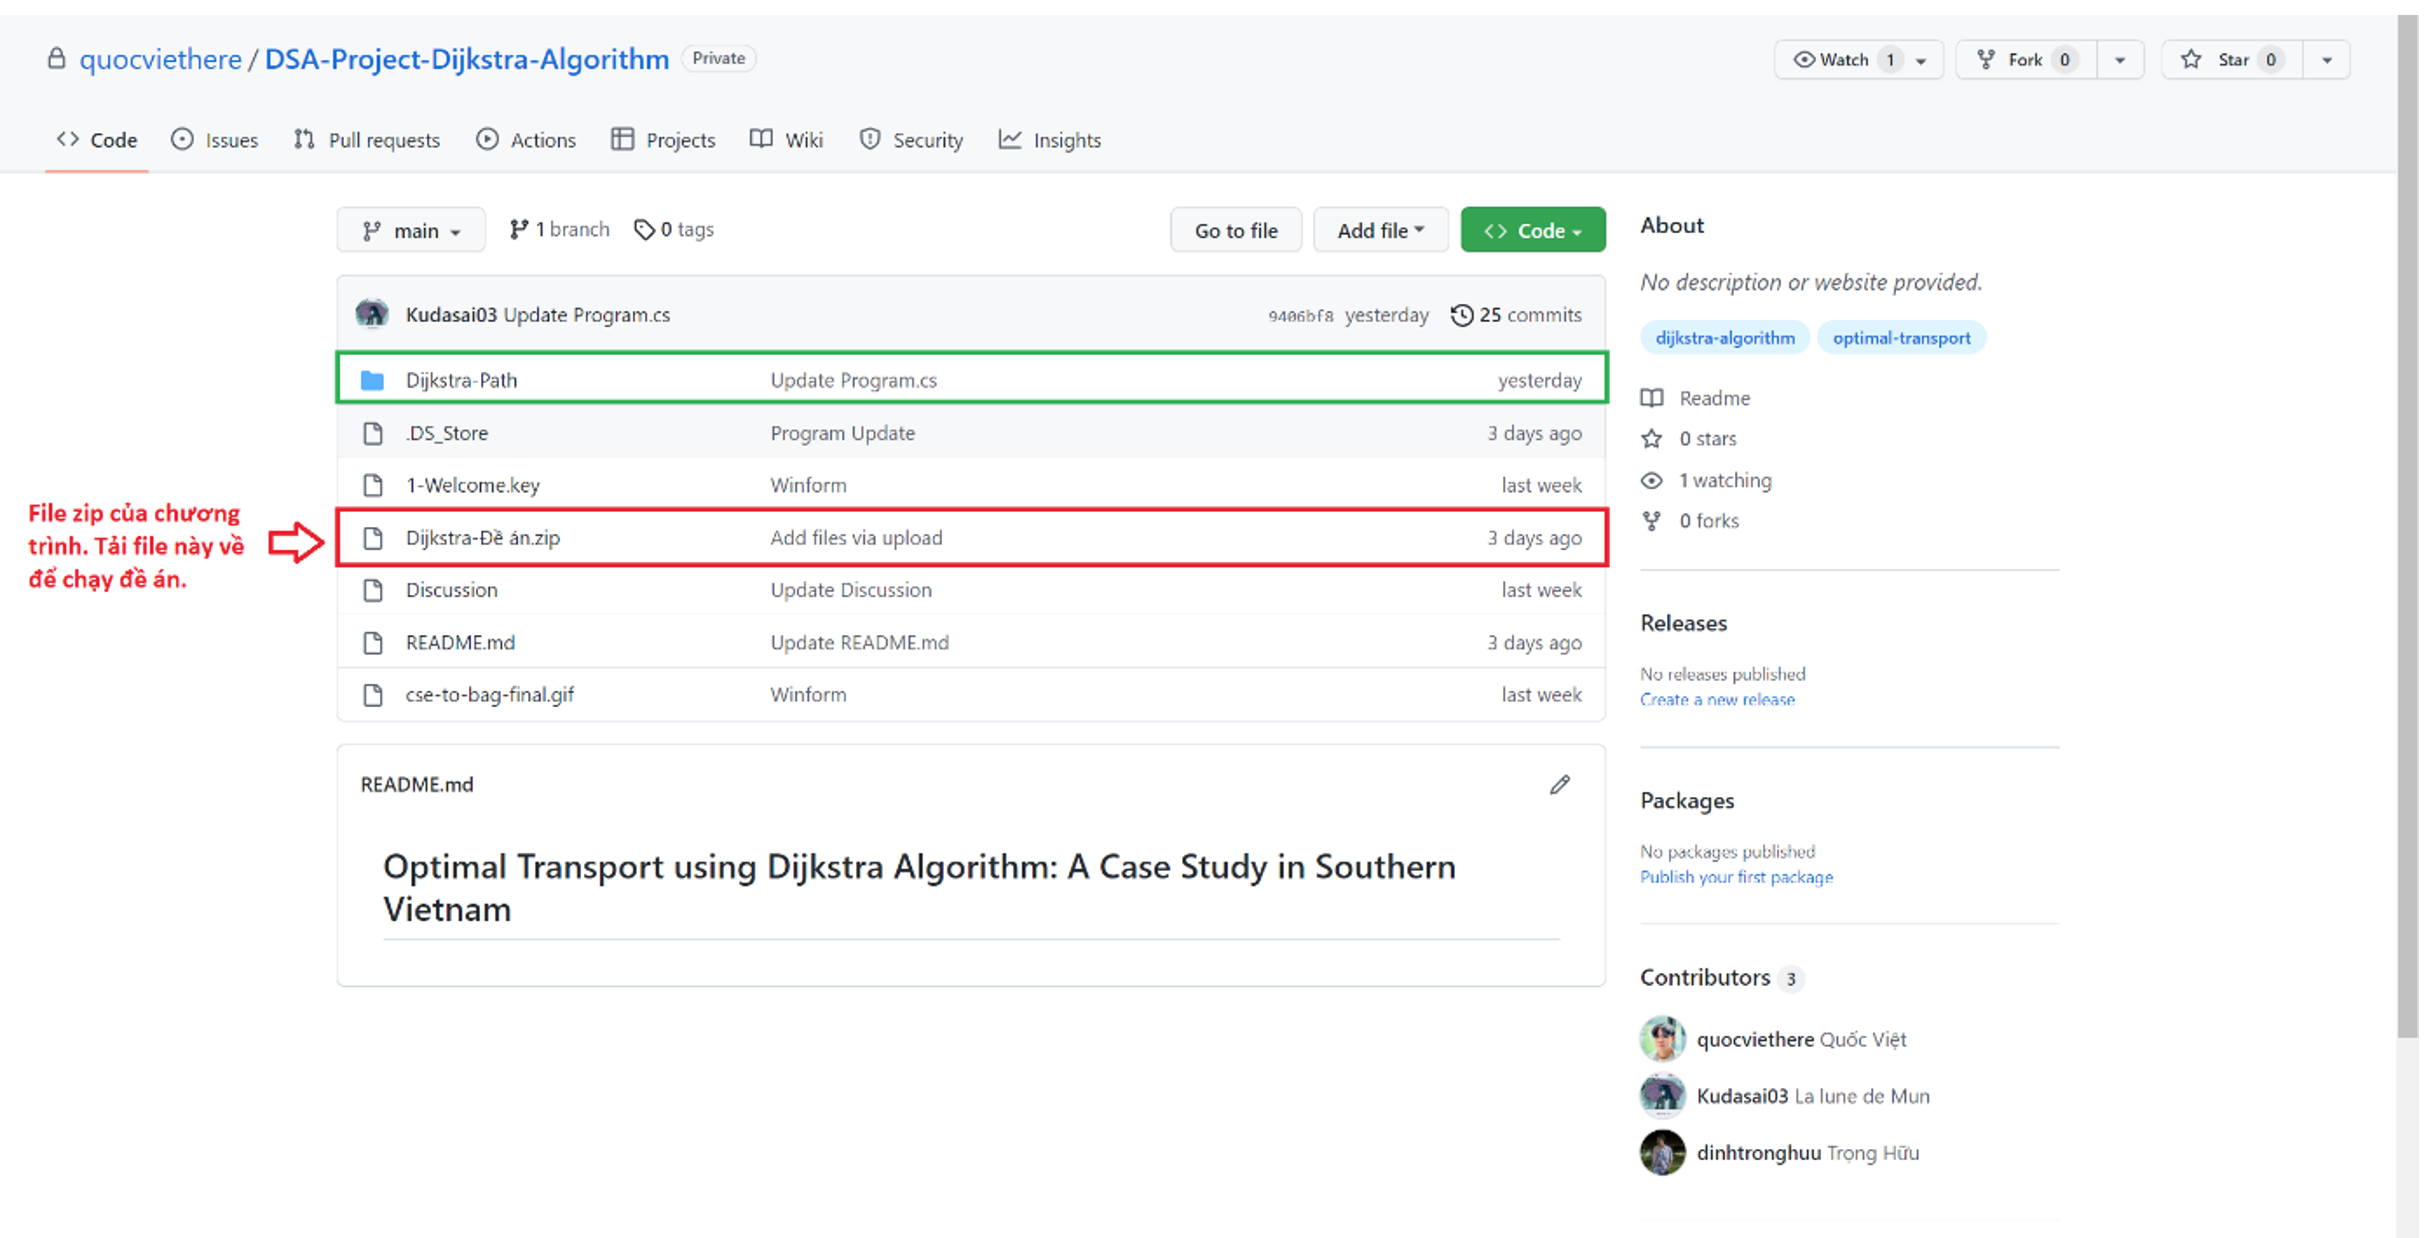
\includegraphics[width=17cm]{5.1.png}
    \caption{Truy cập vào thư mục đề xuất}
\end{figure}

Để biết rõ hơn là chương trình sau khi tải về nằm ở trang nào thì bạn có thể truy cập vào Download (nếu dùng Google Chrome) và ấn vào “Show in folder”.\\

\begin{figure}[!ht]
    \centering
    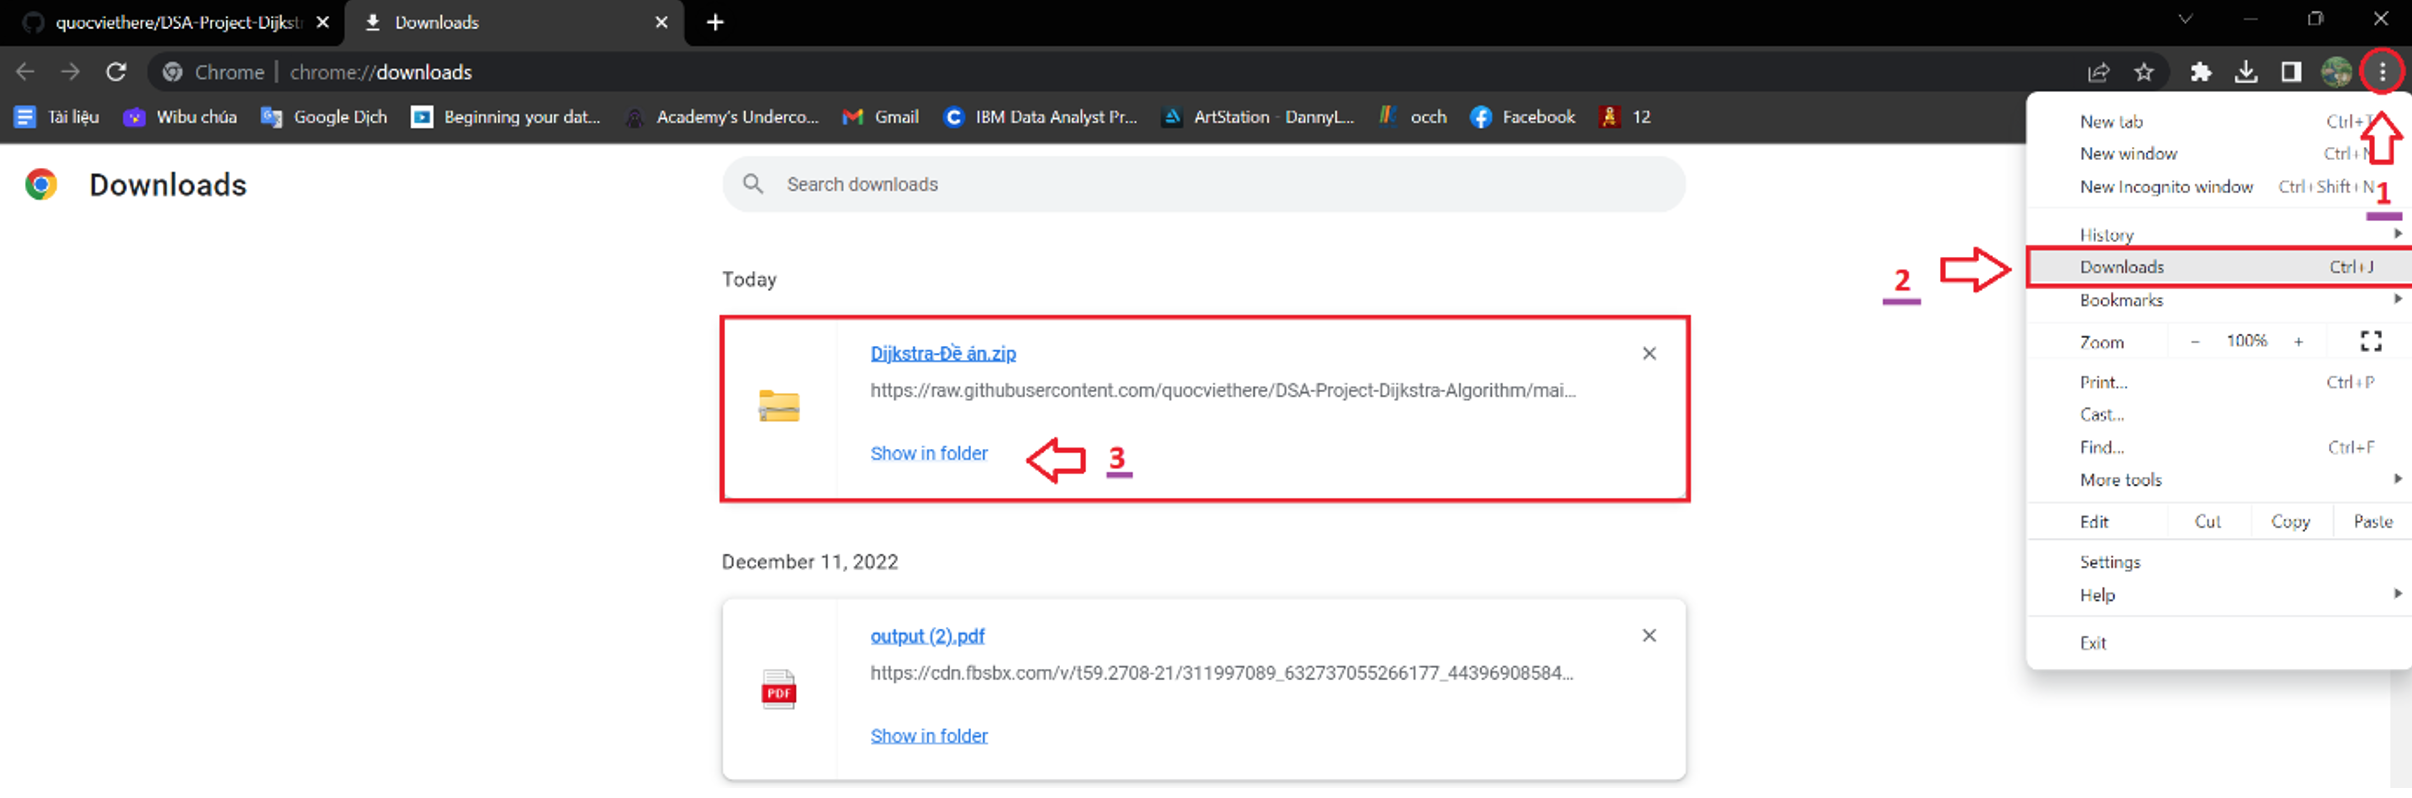
\includegraphics[width=17cm]{5.2.png}
    \caption{Kiểm tra file tải về}
\end{figure}

\textbf{Bước 3:} Cài đặt chương trình.
\begin{itemize}
    \item Sau khi đã tải về và tìm được file nằm ở đâu thì chúng ta tới bước giải nén chương trình.
    \item Tìm tới file vừa tải về. Click chuột phải vào.
    \item Chọn Extract All để giải nén chương trình.
    
    \begin{figure}[!ht]
        \centering
        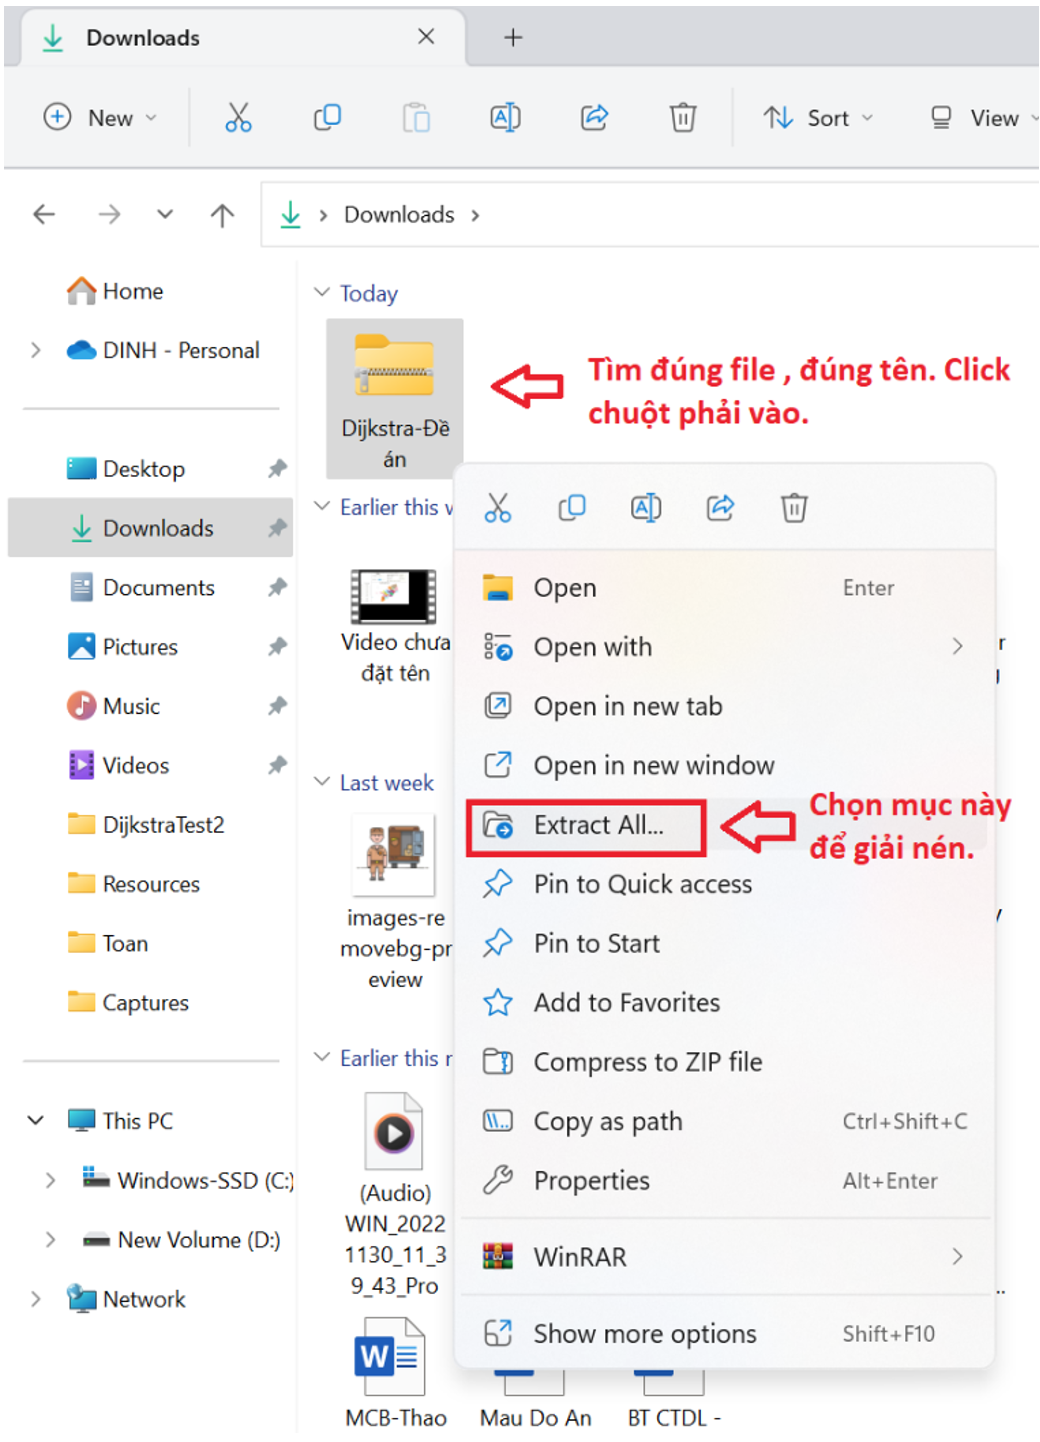
\includegraphics[width=8cm]{5.3.png}
    \end{figure}
    
    \item Tiếp theo một bảng thông báo sẽ hiện ra để chọn thư mục lưu file sau khi giải nén (Tùy người sử dụng).
    
    \begin{figure}[!ht]
        \centering
        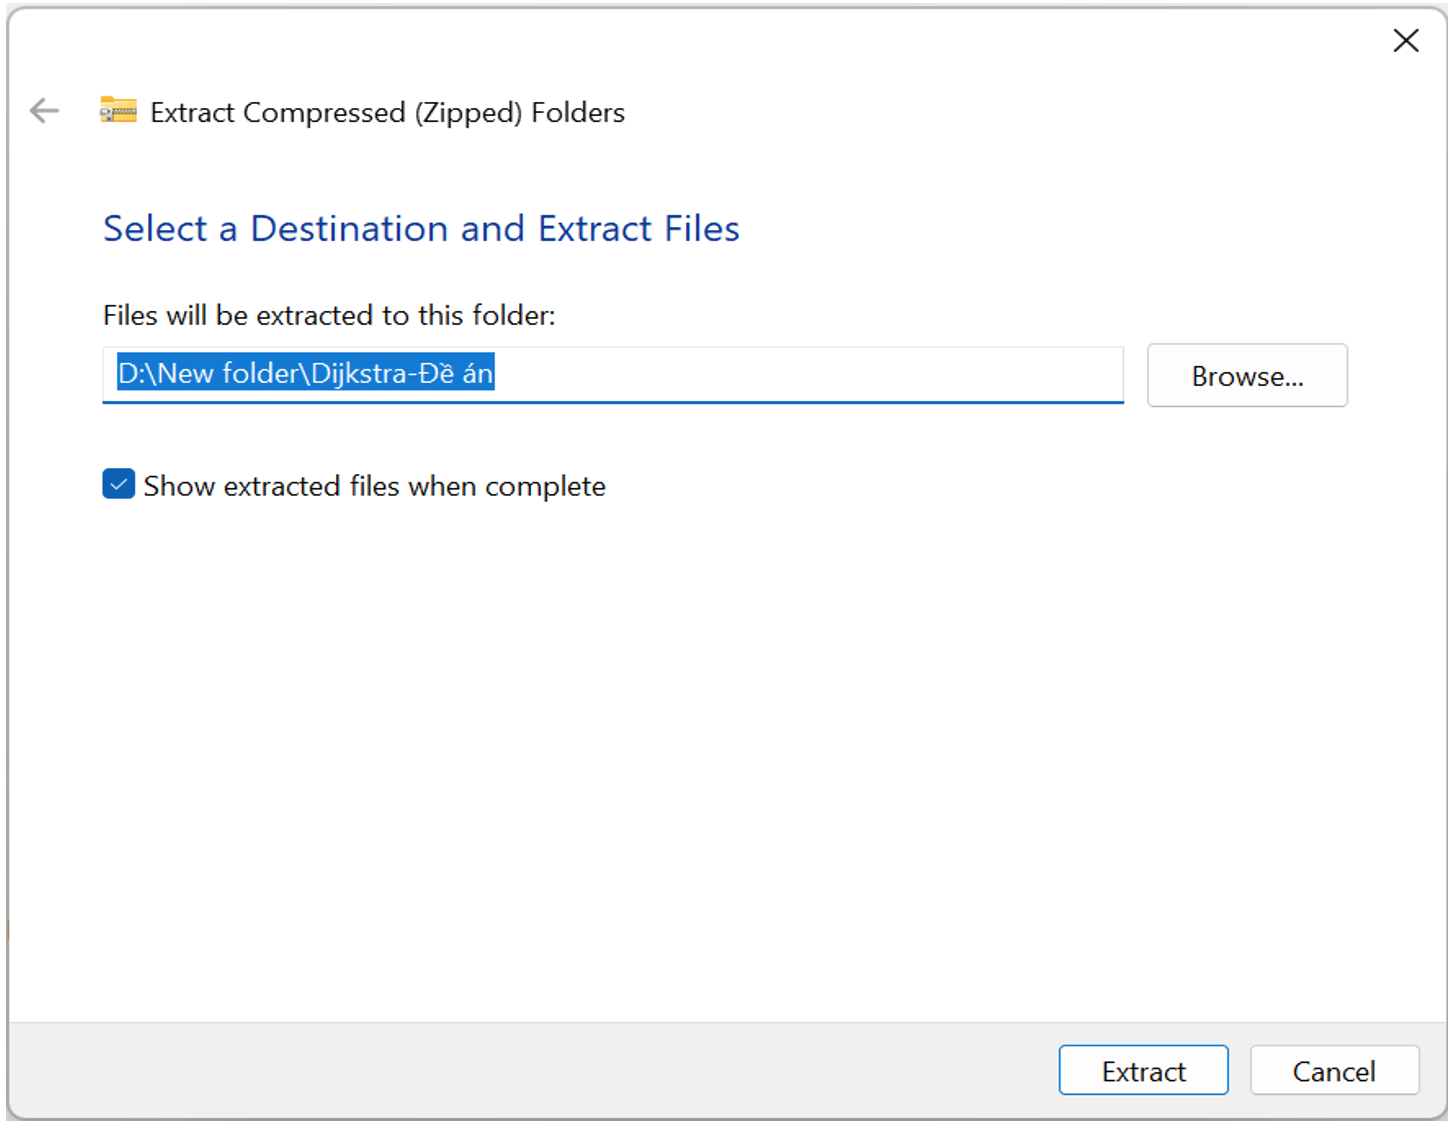
\includegraphics[width=10cm]{5.4.png}
    \end{figure}
    
    \item Sau khi giải nén hoàn thành bạn sẽ được đưa tới thu mục sau khi giải nén. Để chạy chương trình hãy bấm vào ô DijkstraTest2 (đuôi exe).
    
    \begin{figure}[!ht]
        \centering
        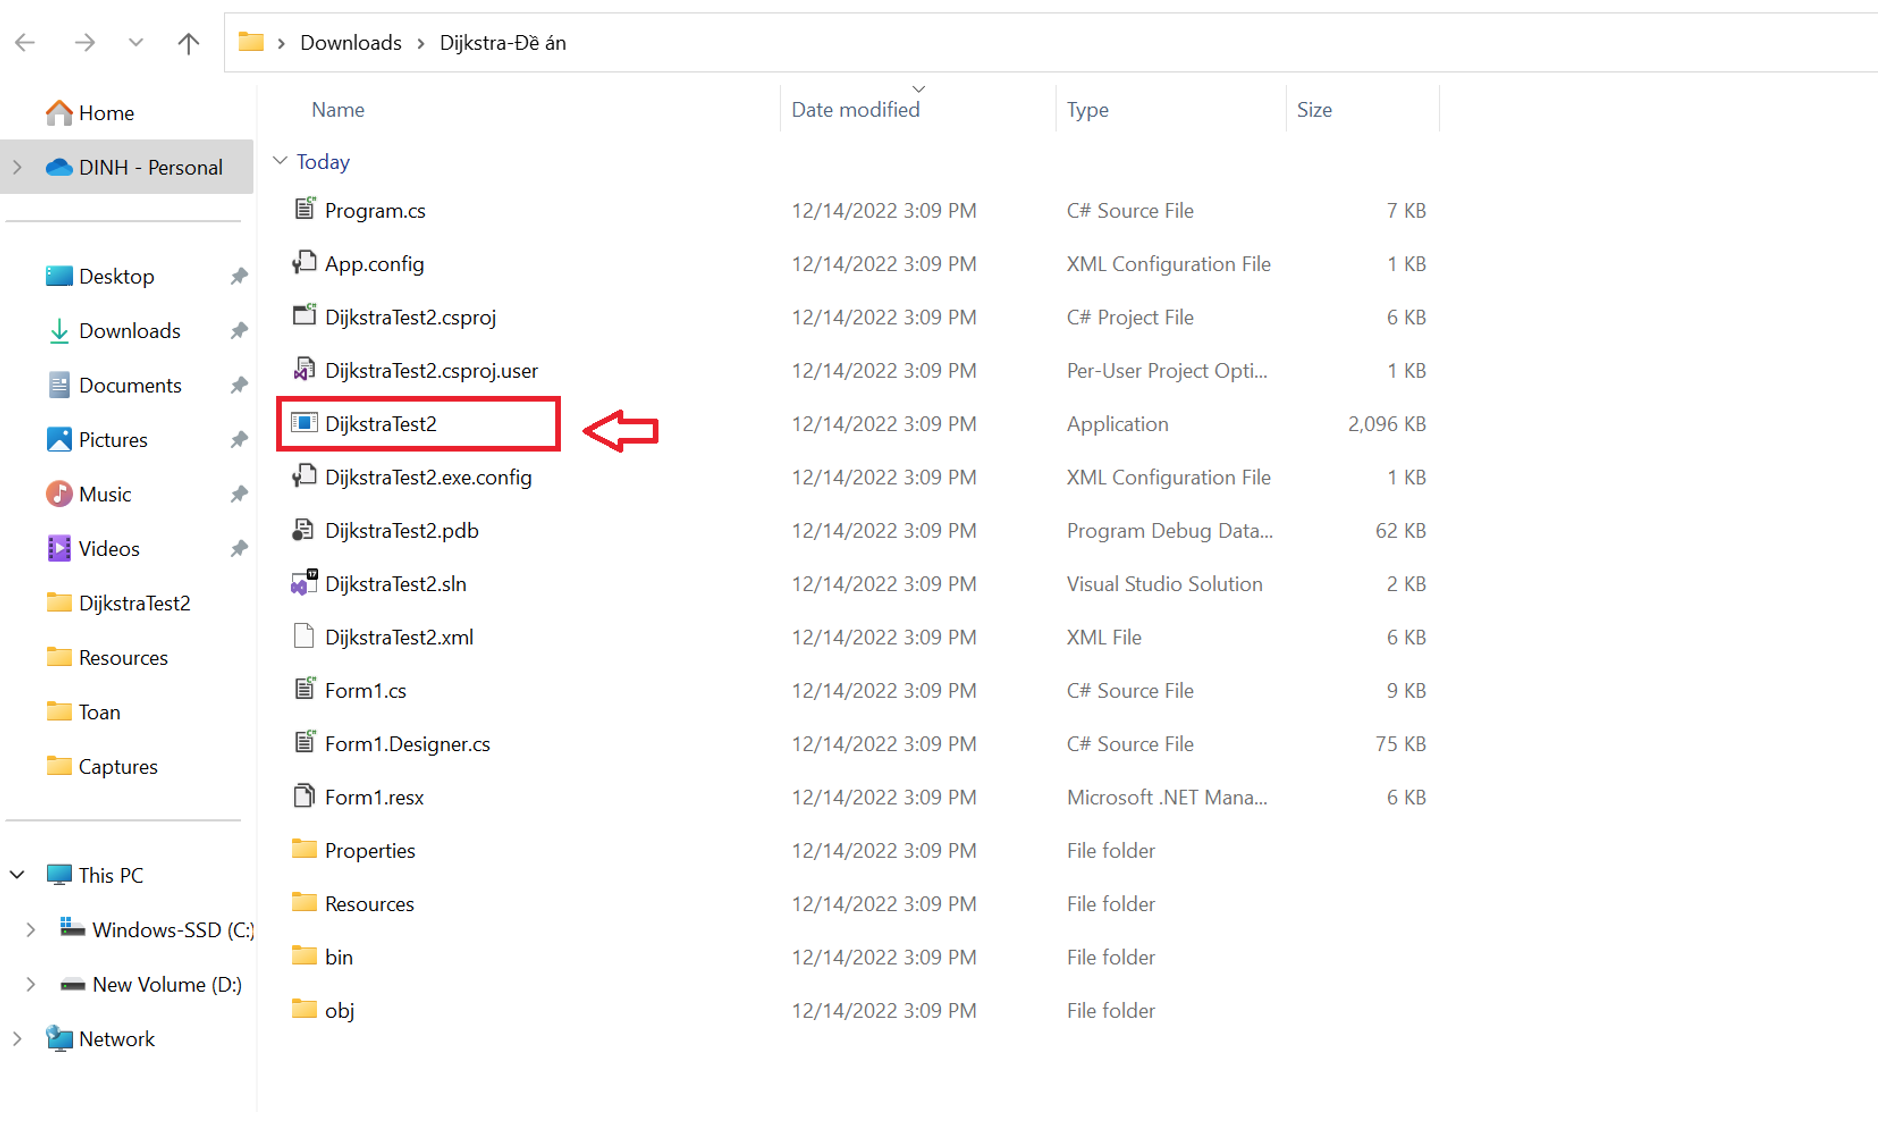
\includegraphics[width=15cm]{5.5.png}
    \end{figure}
    
    \item Nó sẽ ra được giao diện như winform ở phần 3. Và cách sử dụng người dùng có thể quay lại \hyperref[p3]{Mục 3} để xem chi tiết.
    
    \begin{figure}[!ht]
        \centering
        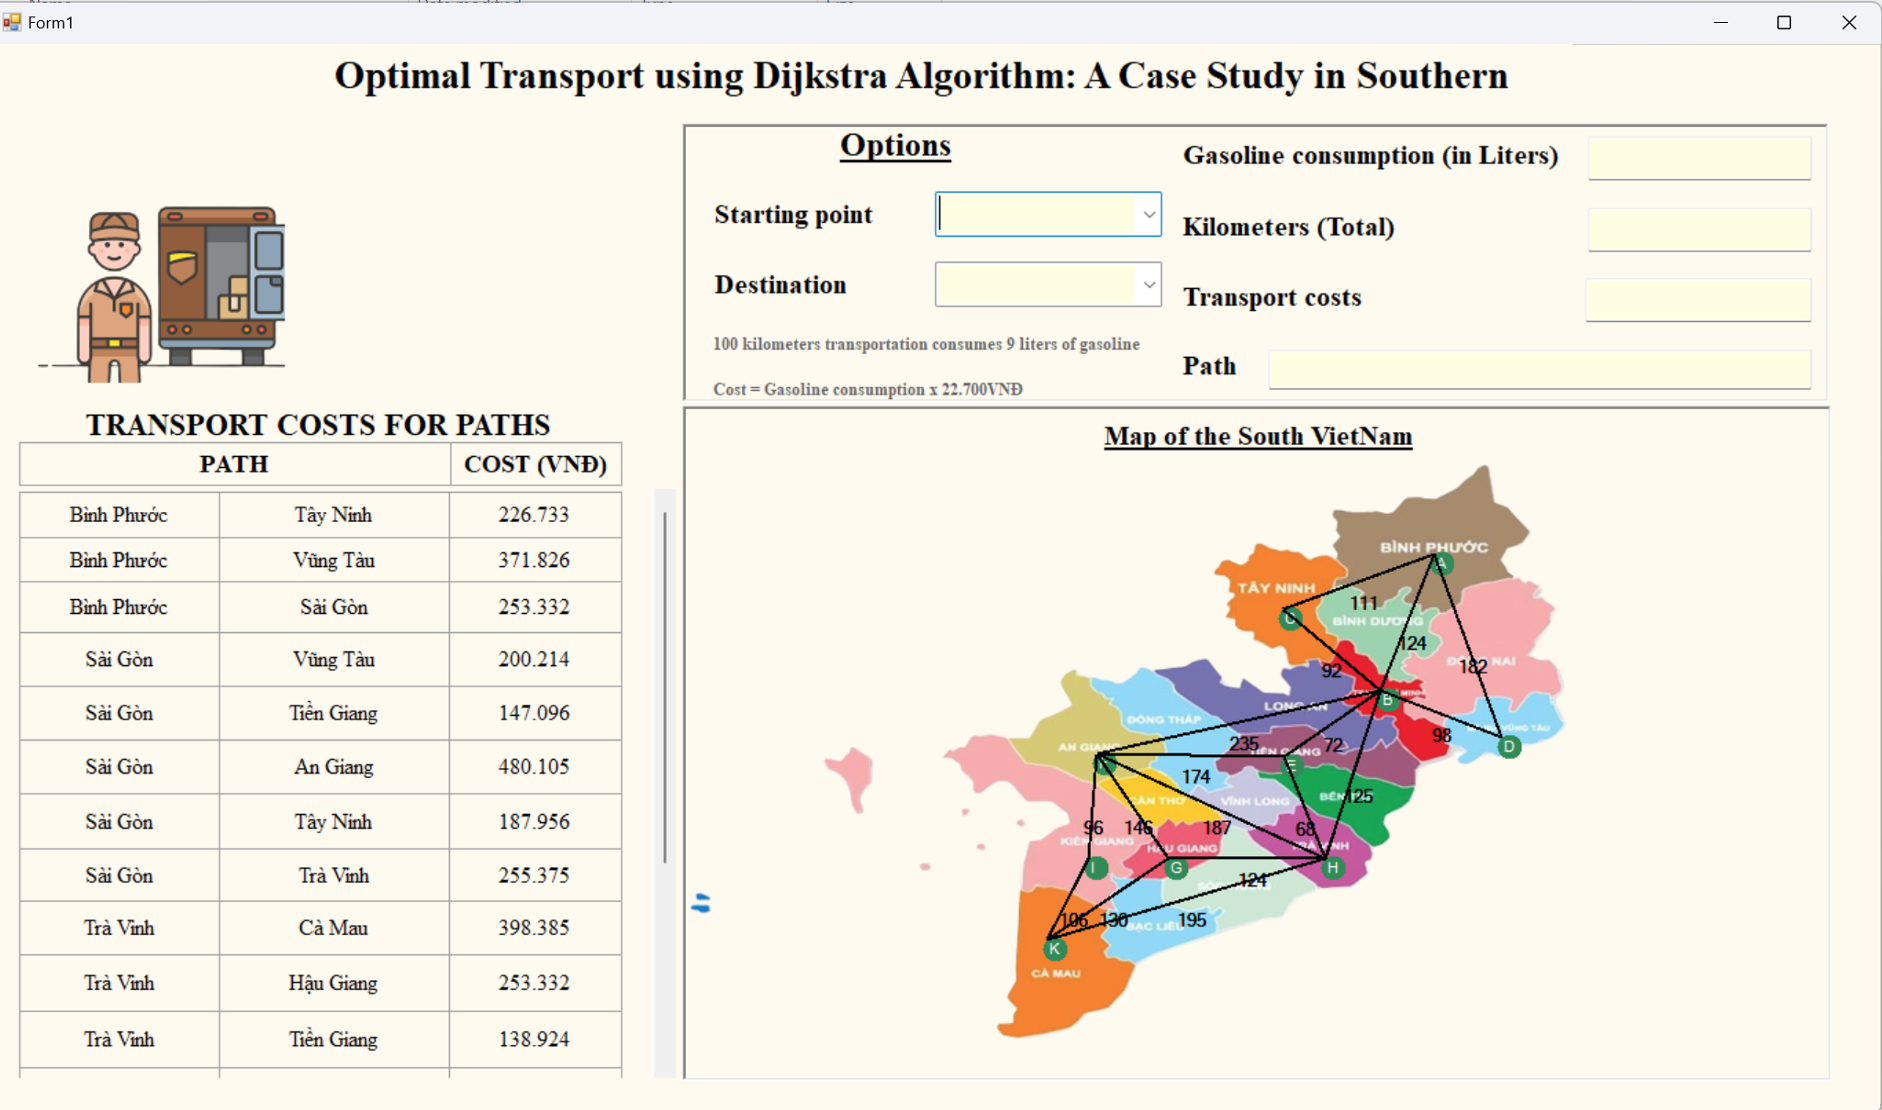
\includegraphics[width=15cm]{5.6.png}
    \end{figure}
\end{itemize}

\subsection{Phân công công việc}

\begin{table}[H]
    \centering
    \begin{tabular}{|l|l|}
    \hline
        \textbf{Thành viên} & \textbf{Nhiệm vụ} \\ \hline
        Nguyễn King & Phân tích và thiết kế lớp, cài đặt thuật toán \\ \hline
        Nguyễn Đình Toàn & Thiết kế giao diện menu chính và giải thích chi tiết chức năng \\ \hline
        Nguyễn Quốc Việt & Khái niệm và trình bày thuật toán \\ \hline
        Đinh Trọng Hữu & Thảo luận, đánh giá về các kết quả nhận được và trình bày hướng phát triển \\ \hline
    \end{tabular}
\end{table}
\vfill

\cite{sedgewick2001algorithms,chen2014path,deng2012fuzzy,javaid2013understanding,schulz2000dijkstra,makariye2017towards,bozyiugit2017public,lanning2014dijkstra,price2020c}
\pagebreak
\bibliographystyle{abbrvnat}
\bibliography{citation}
\end{document}